\documentclass[a4paper]{memoir}

\usepackage{amsmath, amssymb}

\usepackage{paralist}
\usepackage{color}
\usepackage{mathrsfs}
\usepackage{amssymb}
\usepackage{amsmath}
\usepackage{amsfonts}
\usepackage{stmaryrd}
\usepackage{amsthm}
\usepackage{graphicx}
\usepackage{caption}

\newtheorem{theorem}{Theorem}[section]
\newtheorem{lemma}[theorem]{Lemma}
\newtheorem{proposition}[theorem]{Proposition}
\newtheorem{corollary}[theorem]{Corollary}
\newtheorem{claim}[theorem]{Claim}
\newtheorem{subclaim}[theorem]{Subclaim}
\newtheorem{fact}[theorem]{Fact}
\newtheorem{question}[theorem]{Question}

\theoremstyle{definition}
\newtheorem{definition}[theorem]{Definition}
\newtheorem{remark}[theorem]{Remark}
\newtheorem{exercise}[theorem]{Exercise}
\newtheorem{example}[theorem]{Example}

\usepackage[pdftex]{hyperref}
\hypersetup{
    colorlinks=true, %set true if you want coloured links
    linktoc=all,     %set to all if you want both sections and subsections linked
    linkcolor=blue,  %choose some color if you want links to stand out
    allcolors=blue,
}

%general

%for a boxed comment: START
\usepackage[framemethod=tikz]{mdframed}
\newenvironment{boxnote}
{\medskip \begin{mdframed}\begin{scriptsize}}
{\end{scriptsize}\end{mdframed}}
%for a boxed comment: STOP

\newcommand{\cf}{\mathrm{cf}}
\newcommand{\dom}{\mathrm{dom}}
\newcommand{\bb}{\mathbb}
\newcommand{\bbm}{\mathbbm}
\newcommand{\otp}{\mathrm{otp}}
\newcommand{\cof}{\mathrm{cof}}
\newcommand{\nacc}{\mathrm{nacc}}
\newcommand{\acc}{\mathrm{acc}}
\newcommand{\pred}{\mathrm{pred}}
\newcommand{\height}{\mathrm{ht}}
\newcommand{\tp}{\mathrm{tp}}
\newcommand{\ssup}{\mathrm{ssup}}
\newcommand{\lh}{\mathrm{lh}}
\newcommand{\ord}{\mathrm{Ord}}
\newcommand{\mb}{\mathbf}
\newcommand{\mc}{\mathcal}
\newcommand{\power}{\ensuremath{\mathscr{P}}}
\newcommand{\sub}{\subseteq}
\newcommand{\ra}{\rightarrow}

\newcommand{\Add}{\mathrm{Add}}
\newcommand{\Coll}{\mathrm{Coll}}
\newcommand{\R}{\bb{R}}
\newcommand{\Q}{\bb{Q}}
\renewcommand{\P}{\bb{P}}
\newcommand{\B}{\mathcal{B}}
\newcommand{\U}{\bb{U}}
\newcommand{\T}{\bb{T}}
\newcommand{\M}{\bb{M}}
\newcommand{\K}{\bb{K}}

\newcommand{\TP}{{\sf TP}}
\newcommand{\ITP}{{\sf ITP}}
\newcommand{\SP}{{\sf SP}}
\newcommand{\ISP}{{\sf ISP}}
\newcommand{\wTP}{\textsf{wTP}}
\newcommand{\ZFC}{\sf ZFC}
\newcommand{\ZF}{\sf ZF}
\newcommand{\CH}{\sf CH}
\newcommand{\GCH}{\sf GCH}
\newcommand{\SCH}{\sf SCH}
\newcommand{\AC}{\sf AC}
\newcommand{\SR}{{\sf SR}}
\newcommand{\AP}{{\sf AP}}
\newcommand{\PFA}{\sf PFA}
\newcommand{\MA}{\sf MA}
\newcommand{\CP}{\sf CP}
\newcommand{\IGMP}{\sf IGMP}
\newcommand{\wKH}{\sf wKH}
\newcommand{\AGP}{\mathsf{AGP}}
\newcommand{\CF}{\mathsf{CF}}
\newcommand{\SCF}{\mathsf{SCF}}
\newcommand{\NS}{\mathsf{NS}}
\newcommand{\SNS}{\mathsf{SNS}}
\newcommand{\wSP}{\mathsf{wSP}}
\newcommand{\wAGP}{\mathsf{wAGP}}
\newcommand{\GMP}{\mathsf{GMP}}

\synctex = 1

\begin{document}
\frontmatter
\title{Set theory and logic throughout mathematics}
\author{Chris Lambie-Hanson}
\maketitle

\clearpage

\tableofcontents

\mainmatter



\chapter{Lecture 1: Ordinals and the hydra}

\section{Well-orders}

Let us begin by briefly reviewing the definition of \emph{partial order}, 
\emph{linear order}, and \emph{well-order}.

\begin{definition} \label{def: poset}
  Suppose that $X$ is a set and $\leq$ is a binary relation on $X$. Then $\leq$ is a \emph{partial order} 
  on $X$ (or $(X, \leq)$ is a \emph{partial order}) if it is
  \begin{enumerate}
    \item \emph{Reflexive}: $x \leq x$ for all $x \in X$;
    \item \emph{Transitive}: for all $x,y,z \in X$, if $x \leq y$ and $y \leq z$, then $x \leq z$; and
    \item \emph{Anti-symmetric}: for all $x,y \in X$, if $x \leq y$ and $y \leq x$, then $x = y$.
  \end{enumerate}
  A partial order $\leq$ on a set $X$ is a \emph{linear order} if, in addition, it is \emph{total}, i.e., 
  for all $x,y \in X$, we have $x \leq y$ or $y \leq x$.
\end{definition}

If $\leq$ is a partial order on a set $X$ and $x,y \in X$, then we will write $x < y$ to mean that 
$x \leq y$ and $x \neq y$. The relation $<$ is then referred to as the \emph{strict} part of 
$\leq$.

\begin{definition}
  Suppose that $X$ is a set and $R$ is a binary relation on $X$. Then $R$ is \emph{well-founded} if 
  every nonempty subset of $X$ has an $R$-minimal element. In other words, for every nonempty 
  $Y \subseteq X$, there is $y \in Y$ such that, for all $x \in Y$ with $x \neq y$, 
  $\neg (x R y)$. A well-founded linear order is called a \emph{well order}.
\end{definition}

\begin{exercise}
  Suppose that $\leq$ is a linear order on a set $X$. Prove that the following are equivalent.
  \begin{enumerate}
    \item $\leq$ is a well order.
    \item There are no infinite, strictly decreasing sequences with respect to $\leq$. In other 
    words, there does not exist a sequence $\langle x_0, x_1, x_2, \ldots \rangle$ of elements 
    of $X$ such that, for all $n$, we have $x_{n+1} < x_n$.
  \end{enumerate}
\end{exercise}

There is a natural way to assert that two partial orders are ``essentially" the same, i.e., 
\emph{isomorphic}.

\begin{definition}
  Suppose that $\leq_0$ is a partial order on $X_0$ and $\leq_1$ is a partial order on 
  $X_1$. Then we say that $\leq_0$ and $\leq_1$ are \emph{isomorphic} if there is a bijection 
  $F:X_0 \rightarrow X_1$ such that, for all $x,y \in X_0$, we have 
  \[
    x \leq_0 y \Longleftrightarrow F(x) \leq_1 F(y).
  \]
\end{definition}

\begin{example}
  The following are some examples and non-examples of isomorphic partial orders.
  \begin{enumerate}
    \item The open interval $(0,1)$ and the open interval $(0,2)$, both with the usual ordering 
    of real numbers, are isomorphic via the bijection $x \mapsto 2x$.
    \item The open interval $(0,1)$ and the closed interval $[0,1]$ are not isomorphic. One way to 
    see this is to note that $[0,1]$ has a maximal element and $(0,1)$ does not, so any 
    order-preserving map from $(0,1)$ to $[0,1]$ could not include $1$ in its range.
    \item Let $Y$ be any nonempty set. Let $X_0 = \power(Y)$ be the \emph{power set} of $Y$, i.e., 
    the collection of all subsets of $Y$. Let $\leq_0$ be the partial order on $X_0$ defined by 
    letting $u \leq v$ if and only if $u \leq v$.
    
    Let $X_1$ be the collection of all functions $f : Y \rightarrow \{0,1\}$, and let $\leq_1$ 
    be the partial order on $X_1$ defined by letting $f \leq g$ if and only if 
    $f(y) \leq g(y)$ for all $y \in Y$.
    
    Then $\leq_0$ and $\leq_1$ are isomorphic via the bijection $F : X_0 \rightarrow X_1$ that 
    sends each $u \in X_0$ to the \emph{characteristic function} of $u$, i.e., the function 
    $f_u : Y \rightarrow \{0,1\}$ that takes value $1$ on all elements in $u$ and value $0$ on all 
    elements of $Y$ that are not in $u$.
  \end{enumerate}
\end{example}

\section{Ordinal numbers}

Roughly speaking, an ordinal number can be thought of as a description of the order type of a well-order. 
In other words, to each well-order, we assign an ordinal, and two well-orders are isomorphic if and only 
if they are assigned the same ordinal. 

\begin{example}
  For each natural number $n$, all well-orders of size $n$ are isomorphic; their order type is itself 
  referred to as ``$n$". 
  
  However, there are many non-isomorphic countably infinite well-orders. The ordinal describing the 
  order type of the natural numbers,
  \[
    0 < 1 < 2 < 3 < \ldots
  \]  
   is denoted ``$\omega$". But we can form a new order type by adding a new element (call it $\infty$) 
   that is larger than all of the natural numbers:
   \[
     0 < 1 < 2 < 3 < \ldots < \infty.
   \]
   The ordinal describing this order type is denoted ``$\omega + 1$". Or we can form yet another order type 
   by placing two copies of the natural numbers one after the other:
   \[
     0 < 1 < 2 < 3 < \ldots < 0' < 1' < 2' < 3' < \ldots.
   \]
   The ordinal describing this order type is denoted ``$\omega + \omega$".
\end{example}

There is a natural way to order the ordinal numbers themselves. To make this precise, we need the 
following definition.

\begin{definition}
  Suppose that $\leq$ is a well-order of a set $X$. Then an \emph{initial segment} of 
  $(X, \leq)$ is a subset $Y \subseteq X$ such that, for all $y \in Y$ and all $x \in X$, 
  if $x \leq y$, then $x \in Y$. In other words, if $y \in Y$, then $Y$ also contains all elements 
  of $X$ that are smaller than $y$ in the ordering $\leq$.
\end{definition}

\begin{exercise}
  Suppose that $\leq$ is a well-order of a set $X$ and $Y$ is an initial segment of 
  $(X, \leq)$. Then either
  \begin{itemize}
    \item $Y = X$; or
    \item there is $x \in X$ such that $Y = \{y \in X \mid y < x\}$.
  \end{itemize}
\end{exercise}

\begin{exercise} \label{exercise: comp}
  Suppose that $(X_0, \leq_0)$ and $(X_1, \leq_1)$ are two well-orders. Then either
  \begin{enumerate}
    \item $(X_0, \leq_0)$ is isomorphic to an initial segment of $(X_1, \leq_1)$; or
    \item $(X_1, \leq_1)$ is isomorphic to an initial segment of $(X_0, \leq_0)$.
  \end{enumerate}
  If both 1. and 2. hold, then $(X_0, \leq_0)$ and $(X_1, \leq_1)$ are isomorphic.
\end{exercise}

With Exercise \ref{exercise: comp} in mind, we can make the following definition.

\begin{definition}
  Suppose that $\alpha$ and $\beta$ are ordinals. Then we say that $\alpha \leq_{\mathrm{ord}} 
  \beta$ if, whenever $(X_\alpha, \leq_\alpha)$ is a well-order of type $\alpha$ and 
  $(X_\beta, \leq_\beta)$ is a well-order of type $\beta$, then $(X_\alpha, \leq_\alpha)$ 
  is isomorphic to an initial segment of $(X_\beta, \leq_\beta)$.
\end{definition}

\begin{exercise}
  The class of ordinals is well-ordered by $\leq_{\mathrm{ord}}$.
\end{exercise}

One can perform arithmetic on ordinal numbers. We will make this more precise later, but let 
us first give an informal description. Let $\alpha$ and $\beta$ be ordinal numbers, 
and let $(X_\alpha, \leq_\alpha)$ and $(X_\beta, \leq_\beta)$ be well-orders of type 
$\alpha$ and $\beta$, respectively.

We first describe ordinal addition. The ordinal $\alpha + \beta$ is the 
ordinal describing the well-ordering formed by placing a copy of $(X_\beta, \leq_\beta)$ 
after a copy of $(X_\alpha, \leq_\alpha)$ (i.e., every element of $X_\beta$ is declared to 
be larger than every element of $X_\alpha$). 

Note that ordinal addition is not commutative: it may not be the case that $\alpha + \beta = 
\beta + \alpha$. To see this, consider $2 + \omega$ and $\omega + 2$. Represent the ordinal 
$2$ by the order $0' < 1'$, and represent $\omega$ by the usual natural numbers. Then 
$2 + \omega$ is the order type of the order
\[
  0' < 1' < 0 < 1 < 2 < 3 < \ldots
\]
This is isomorphic to the usual ordering of the natural numbers, via the map 
\begin{align*}
  0' & \mapsto 0 \\
  1' & \mapsto 1 \\ 
  n & \mapsto n + 2 \text{ for every natural number } n.
\end{align*}
Thus, $2 + \omega = \omega$. On the other hand, $\omega + 2$ is the order type of the order
\[
  0 < 1 < 2 < \ldots < 0' < 1'
\]
This is clearly \emph{not} isomorphic to the natural numbers; for example, it has a maximal element, 
whereas that natural numbers do not. Thus, $\omega + 2 \neq \omega$, and in fact 
$\omega <_{\mathrm{ord}} \omega + 2$.

We next describe ordinal multiplication. The ordinal 
$\alpha \cdot \beta$ is the ordinal describing the well-ordering formed by starting with a copy of 
$(X_\beta, \leq_\beta)$ and replacing every element of $X_\beta$ with a copy of 
$(X_\alpha, \leq_\alpha)$.

Again, ordinal multiplication is not commutative. For example, $2 \cdot \omega$ is the order type 
of the following order:
\[
  0 < 0' < 1 < 1' < 2 < 2' < 3 < 3' < \ldots
\]
formed by replacing every natural number $n$ with a copy $n < n'$ of the two-element order.
It is not too hard to show that this order is isomorphic to the natural numbers, so 
$2 \cdot \omega = \omega$. On the other hand, $\omega \cdot 2$ is the order type of the following order:
\[
  0 < 1 < 2 < 3 < \ldots < 0' < 1' < 2' < 3' < \ldots
\]
formed by replacing each element of the two-element order $\ast < \ast'$ by a copy of the natural 
numbers. This is not isomorphic to the set of natural numbers; for instance, it contains elements 
that are larger than infinitely many other elements, whereas the natural numbers do not. 
Thus, $\omega \cdot 2 \neq \omega$, and in fact $\omega <_{\mathrm{ord}} \omega \cdot 2$.

We finally describe ordinal exponentiation. If $\alpha = 0$, then $\alpha^\beta = 0$. 
Otherwise, first let $0_\alpha$ denote the 
\emph{minimal} element of $(X_\alpha, \leq_\alpha)$. This must exist, since $\leq_\alpha$ 
is a well-order. We say that a function $f: X_\beta \rightarrow X_\alpha$ is \emph{finitely 
supported} if the set $\{y \in X_\beta \mid f(y) \neq 0_\alpha\}$ is finite. The ordinal 
$\alpha^\beta$ is now defined as follows. Let $Z$ be the set of all finitely-supported 
functions from $X_\beta$ to $X_\alpha$. Now describe an ordering $\preceq$ on $Z$ as follows. 
Given $f,g \in Z$, set $f \preceq g$ if and only if either
\begin{itemize}
  \item $f = g$; or
  \item $f \neq g$ and, letting $y \in X_\beta$ be the $\leq_\beta$-maximal element such that 
  $f(y) \neq g(y)$, we have $f(y) \leq_\alpha g(y)$.
\end{itemize}
Then let $\alpha^\beta$ be the ordinal describing the order type of $(Z, \preceq)$.

\begin{exercise}
  Prove that the order $(Z, \preceq)$ described in the preceding paragraph is indeed a well-order.
\end{exercise}

\subsection{A concrete representation of the ordinals.}

In practice we often work with a particular concrete realization of the ordinals, and we 
think of an ordinal $\alpha$ as the set of all ordinals that are strictly less than $\alpha$ 
(with respect to the ordering $\leq_{\mathrm{ord}}$ introduced above. At first glance, this 
may appear like a circular definition, but it is not, due to the fact that $\leq_{\mathrm{ord}}$ 
is itself a well-ordering. In particular, there is a least ordinal, $0$. Since there are no ordinals 
strictly less than $0$, we represent $0$ as the empty set, $\emptyset$. The next smallest ordinal 
is $1$. It only has one ordinal less than it, namely, $0$, so $1$ is represented as 
$\{0\} = \{\emptyset\}$. The first few ordinals are thus represented as follows:
\begin{align*}
  0 &= \emptyset \\
  1 &= \{0\} = \{\emptyset\} \\ 
  2 &= \{0,1\} = \{\emptyset, \{\emptyset\}\} \\ 
  3 &= \{0,1,2\} = \{\emptyset, \{\emptyset\}, \{\emptyset, \{\emptyset\}\}\} \\ 
  4 &= \{0,1,2,3\} = \{\emptyset, \{\emptyset\}, \{\emptyset, \{\emptyset\}\}, 
  \{\emptyset, \{\emptyset\}, \{\emptyset, \{\emptyset\}\}\}\} \\ 
  &\ldots \\ 
  \omega &= \{0,1,2,3,4, \ldots\} \\ 
  \omega + 1 &= \omega \cup \{\omega\} = \{0,1,2,3,4, \ldots\} \cup \{\omega\} \\ 
  \omega + 2 &= \omega \cup \{\omega, \omega + 1\} \\ 
  &\ldots \\ 
  \omega + \omega &= \omega \cdot 2 = \{0,1,2,3,4, \ldots\} \cup \{\omega, \omega + 1, \omega + 2, 
  \omega + 3, \omega + 4, \ldots\}
\end{align*}

\begin{center}
  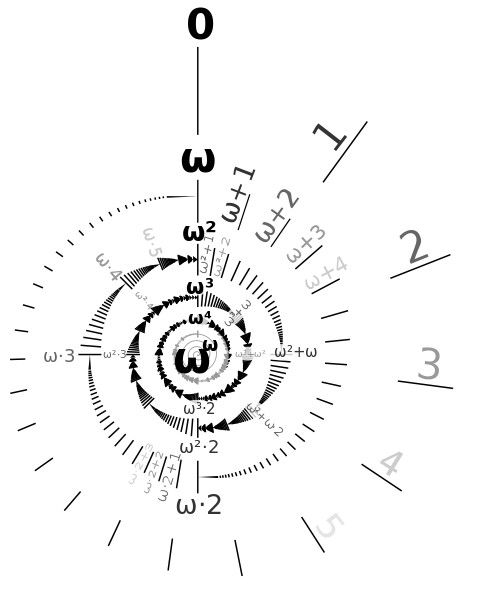
\includegraphics[width=3in]{omega_to_omega}
  \captionof{figure}{A stylized image of the ordinals up to $\omega^\omega$}
\end{center}

With this concrete representation of the ordinals, we can easily be more precise about 
ordinal arithmetic. We first introduce the following notions.

\begin{definition}
  Let $X$ be a nonempty set of ordinals. Then the \emph{supremum} of $X$, denoted 
  $\sup(X)$, is the least ordinal that is greater than or equal to every element of $X$.
\end{definition}

\begin{exercise}
  Working with our concrete representation of the ordinals, prove that, for every nonempty 
  set of ordinals $X$, the supremum of $X$ is equal to the union of all of the elements of 
  $X$, i.e., 
  \[
    \sup(X) = \bigcup X.
  \]
\end{exercise}

\begin{definition}
  Suppose that $\beta$ is an ordinal.
  \begin{enumerate}
    \item We say that $\beta$ is a \emph{successor} ordinal if $\beta = \alpha + 1$ for some 
    ordinal $\alpha$.
    \item If $\beta$ is not a successor ordinal, we say that $\beta$ is a \emph{limit} 
    ordinal.
  \end{enumerate}
\end{definition}

We can now rigorously define ordinal arithmetic by recursion. We first deal with addition. 
For all ordinals $\alpha$, we let:
\begin{itemize}
  \item $\alpha + 0 = \alpha$;
  \item $\alpha + 1 = \alpha \cup \{\alpha\}$;
  \item for all ordinals $\beta$, we have $\alpha + (\beta + 1) = (\alpha + \beta) + 1$;
  \item if $\gamma$ is a nonzero limit ordinal, then 
  $\alpha + \gamma = \sup\{\alpha + \beta \mid \beta < \gamma\}$.
\end{itemize}
Next, multiplication:
\begin{itemize}
  \item $\alpha \cdot 0 = 0$;
  \item $\alpha \cdot 1 = \alpha$;
  \item for all ordinals $\beta$, we have $ \alpha \cdot (\beta + 1) = (\alpha \cdot \beta) + \alpha$;
  \item if $\gamma$ is a nonzero limit ordinal, then 
  $\alpha \cdot \gamma = \sup\{\alpha \cdot \beta \mid \beta < \gamma\}$.
\end{itemize}
Finally, exponentiation:
\begin{itemize}
  \item $\alpha^0 = 1$;
  \item $\alpha^1 = \alpha$;
  \item for all ordinals $\beta$, we have $\alpha^{\beta + 1} = (\alpha^\beta) \cdot \alpha$;
  \item if $\gamma$ is a nonzero limit ordinal, then
  $\alpha^\gamma = \sup\{\alpha^\beta \mid \beta < \gamma\}$.
\end{itemize}

\section{The hydra}

We end this first lecture with a surprising demonstration of the utility of infinite ordinals: 
the hydra game. You may be familiar with the Hydra from Greek mythology. It is a fearsome water 
monster with many heads with the property that, whenever you chop off one of its heads, two 
heads will grow back in its place. Eventually, the hydra was slain by Heracles, with the 
assistance of his nephew Iolaus.

We will be examining a game played using a mathematical version of the Hydra introduced in the paper 
``Accessible independence results for Peano Arithmetic" by Laurie Kirby and Jeff Paris. For us, a \emph{hydra} 
is a finite tree with a root. In other words, a hydra consists of finitely many nodes and edges. 
There is a root node at the bottom, which has finitely many edges coming out of it, each leading 
to another node. In turn, each of these nodes has finitely many edges coming out of it, each 
leading to a further node, and so on. For example, this is a hydra:
\begin{center}
  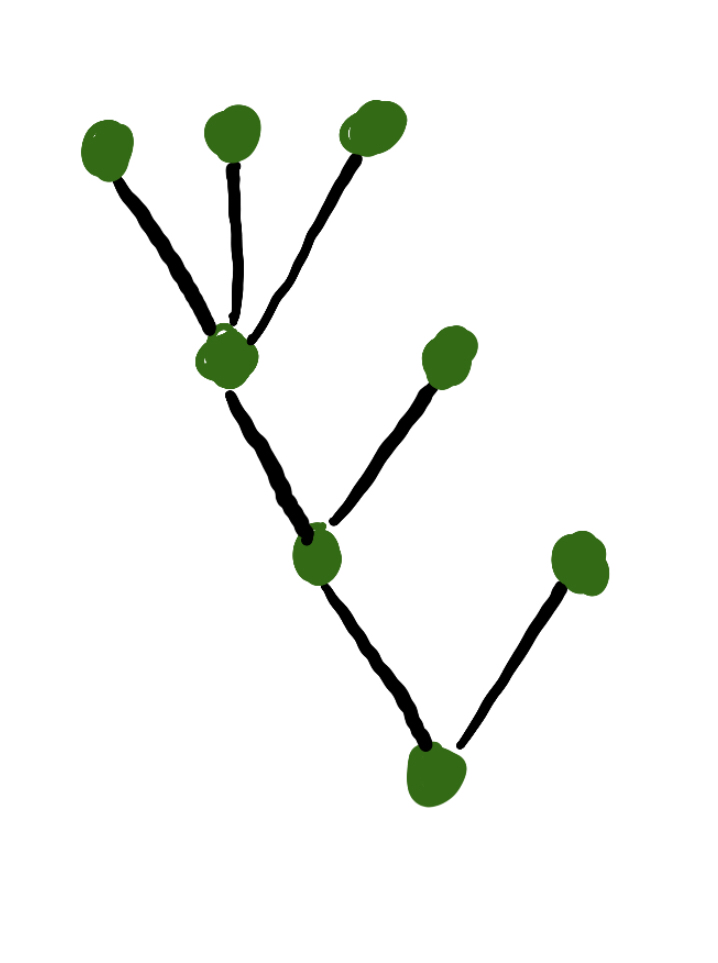
\includegraphics[width=2in]{Hydra1}
  \captionof{figure}{A hydra}
\end{center}

We will always draw hydras with the root at the bottom. A \emph{terminal node} of a hydra is a 
non-root node that is connected to only one other node. A \emph{head} of a hydra consists of a 
terminal node and the single edge that leads to it. For example, the hydra pictured above has 
five heads:
\begin{center}
  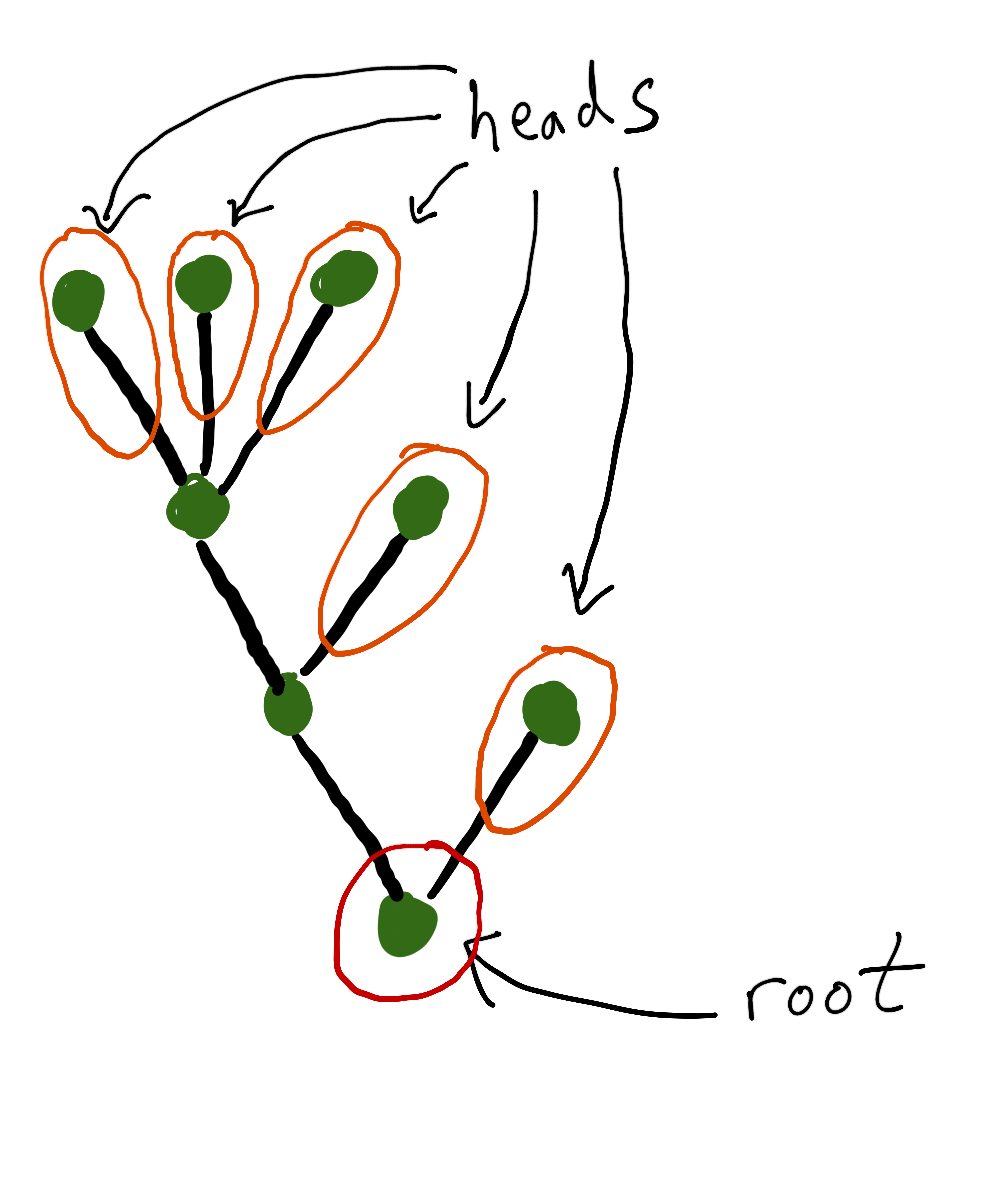
\includegraphics[width=2in]{Hydra2}
  \captionof{figure}{A hydra with its root and heads labeled}
\end{center}

Given a head, the single node that it is attached to is called its \emph{parent}. If its 
parent is not the root, then the node that is one step closer to the root from its parent 
is called its \emph{grandparent}:
\begin{center}  
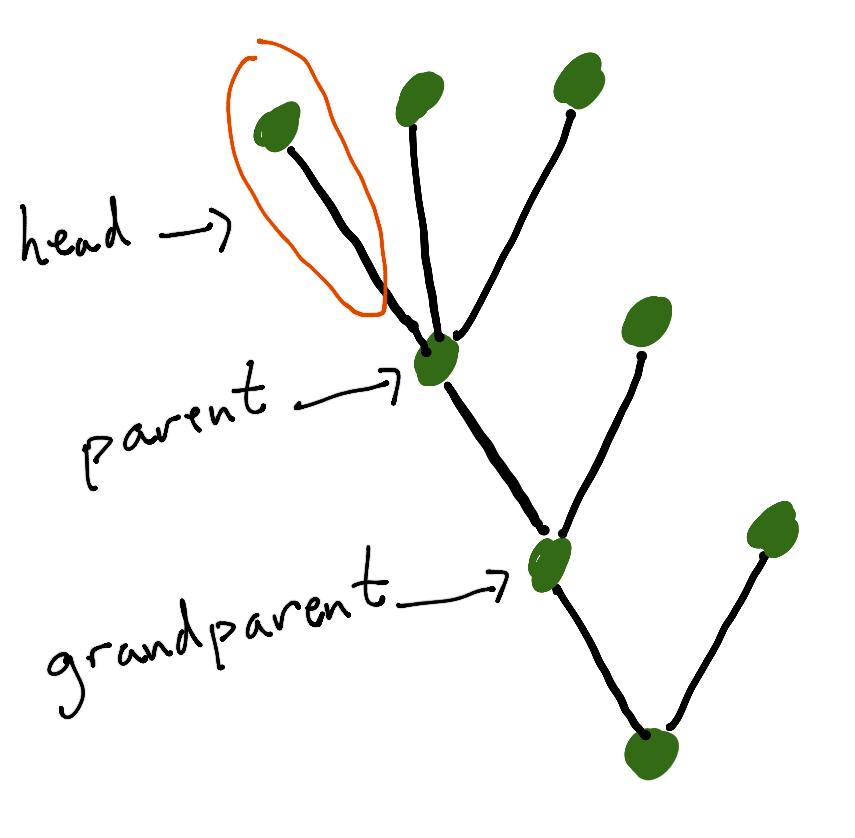
\includegraphics[width=2in]{HydraFamily}
  \captionof{figure}{A hydra with a labeled head, its parent, and its grandparent}
\end{center}

In the hydra game, we start with a hydra and, on each move (starting with Move 1), we chop off 
one of its heads. Our goal is to reduce the hydra to only a root node in a finite number of moves. 
However, like its mythological counterpart, the hydra regenerates, according to the following rules:
\begin{itemize}
  \item If, on Move $n$, we chop off a head directly connected to the root, then the hydra does not 
  create any new heads.
  \item If, on Move $n$, we chop off a head \emph{not} directly connected to the root, then 
  first delete the node and edge that make up that head. Then, move down one edge towards the 
  root, to the edge connecting the parent and the grandparent of the head that was removed. 
  The hydra makes $n$ new copies of the subtree consisting of this edge and everything above it 
  and attaches each of these new copies to the grandparent of the head that was removed.
\end{itemize}

This is best illustrated with a picture. Suppose that we are about to make Move 2 of a game, and we 
are confronted with the hydra pictured above. One option is to chop off the head in the bottom 
right, directly connected to the root:
\begin{center}
  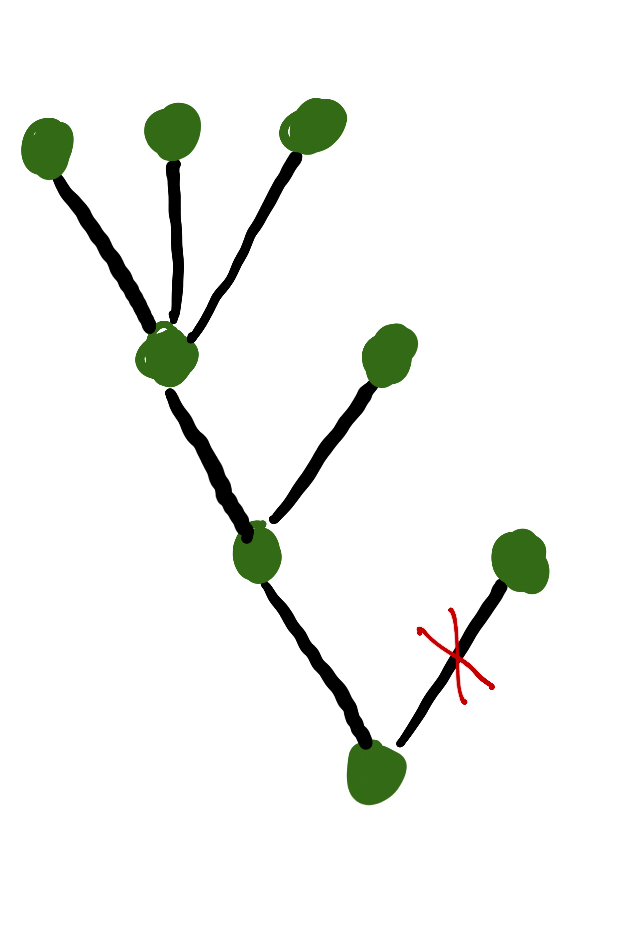
\includegraphics[width=1.5in]{Hydra3}
  \captionof{figure}{Chopping off a head directly connected to the root}
\end{center}

Since this head is directly connected to the root, the hydra does not generate any new heads, 
so on our next move we see the following hydra:
\begin{center}
  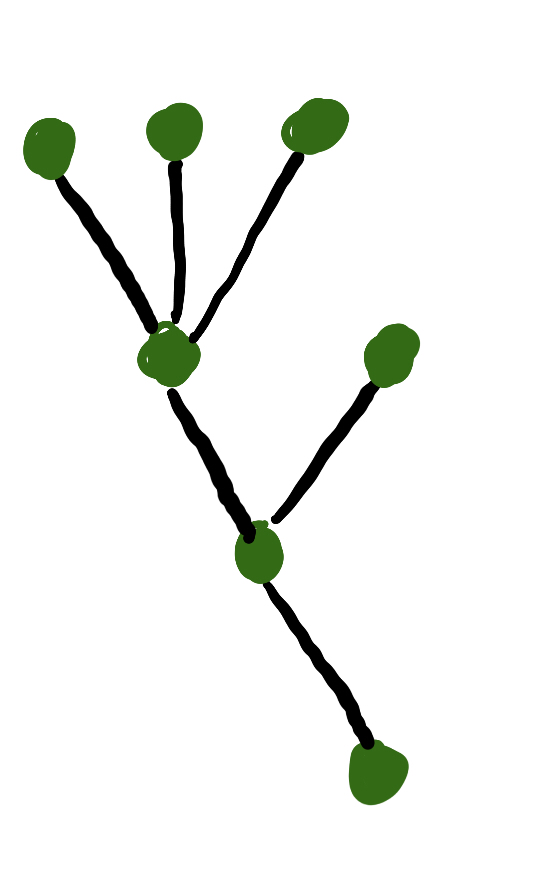
\includegraphics[width=1.5in]{Hydra4}
  \captionof{figure}{The result of the move in Figure 1.5}
\end{center}

However, we could have done something different on Move 2 and instead chopped off the head 
on the upper left:
\begin{center}
  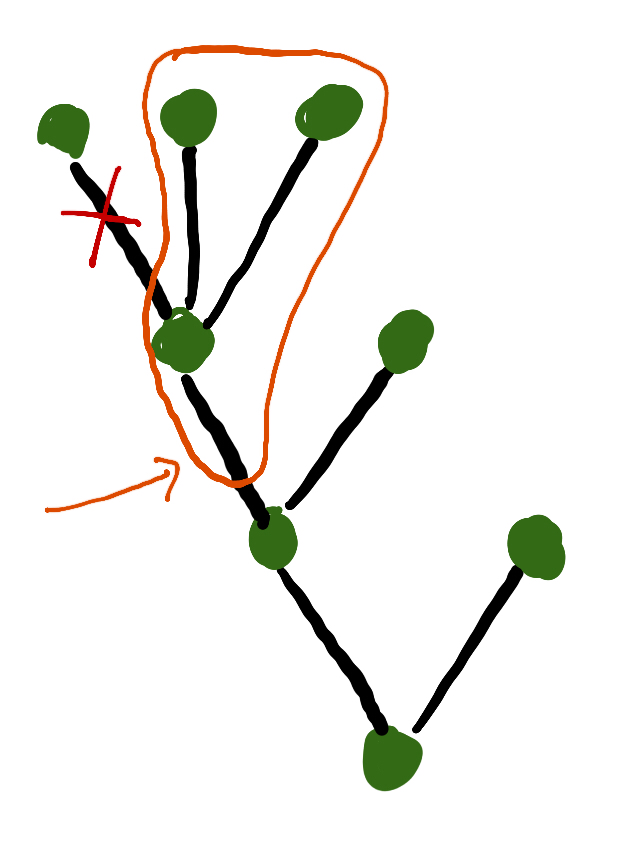
\includegraphics[width=1.5in]{Hydra6}
  \captionof{figure}{Chopping off a head not directly connected to the root}
\end{center}
Now, to generate the hydra for the next move, we first remove the head. Then we consider 
the subtree consisting of the edge between the head's parent and grandparent and 
everything above it (circled in orange in Figure 1.6). Since we are on Move 2, we make 2 new copies of 
it and attach them to the grandparent of the removed head, resulting in the following hydra:
\begin{center}
  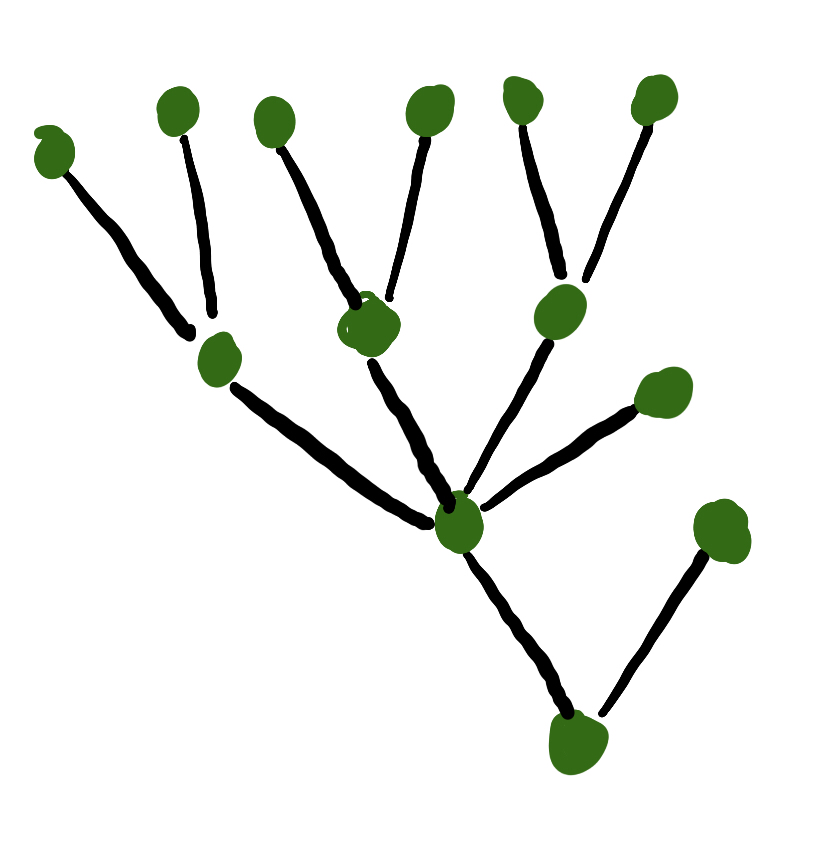
\includegraphics[width=1.5in]{Hydra7}
  \captionof{figure}{The result of making the move in Figure 1.7 on Move 2}
\end{center}

Let us see now a complete play of the game, starting from a very simple hydra:
\begin{center}
  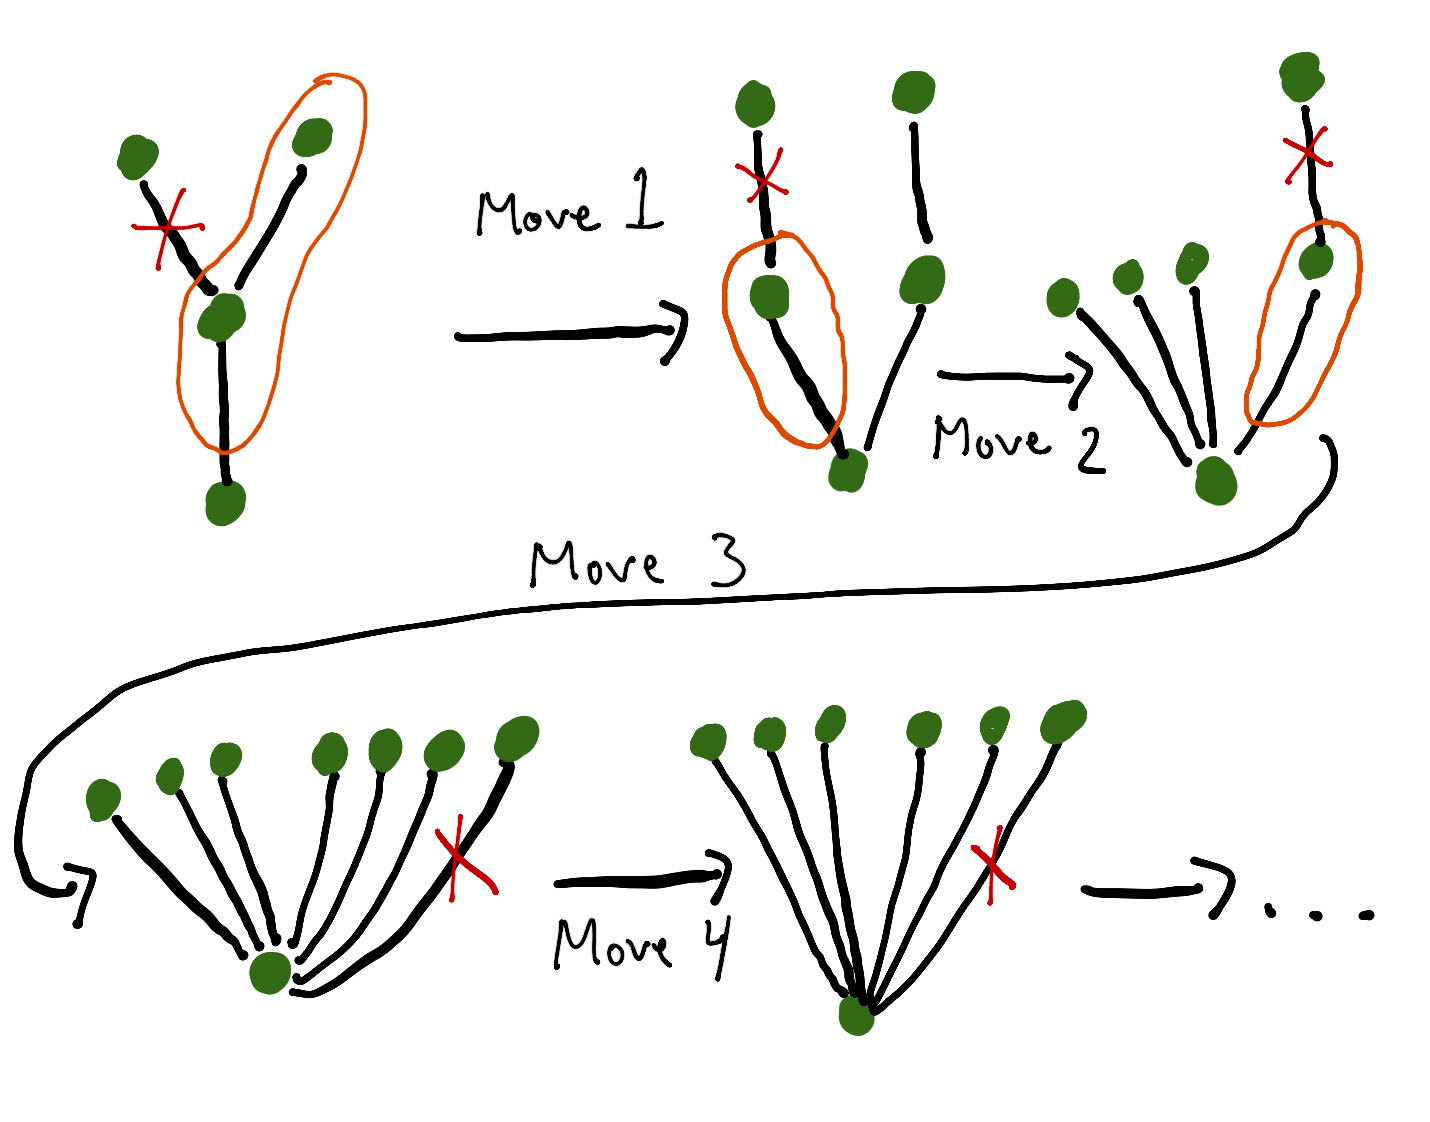
\includegraphics[width=4in]{Hydra11}
  \captionof{figure}{A play of the hydra game}
\end{center}

We begin with a simple hydra with two heads. In Move 1, we chop off the left head. 
The head is not connected to the root, so we make one new copy of the circled region 
and connect it to the head's grandparent (which in this case is the root). The hydra 
we are left with still has two heads. In Move 2, we chop off the left head. Again, this 
is not connected to the root, so we make two new copies of the circled region and connect 
them them to the head's grandparent. In Move 3, we chop off the right head (the only one 
left that is not directly connected to the root). We make three new copies of the circled 
region and connect them to the head's grandparent. We are then left with a hydra that has 
seven heads, but each of them is directly connected to the root. We can thus chop them off 
one at a time, winning the game after seven more moves.

We thus won this round of the hydra game, but maybe that is only because we started with a 
very simple hydra. Consider the following diagram, taken from the paper by Kirby and 
Paris in which the hydra game was introduced, depicting the first three moves in a hydra 
game starting from a more complicated hydra:

\begin{center}
  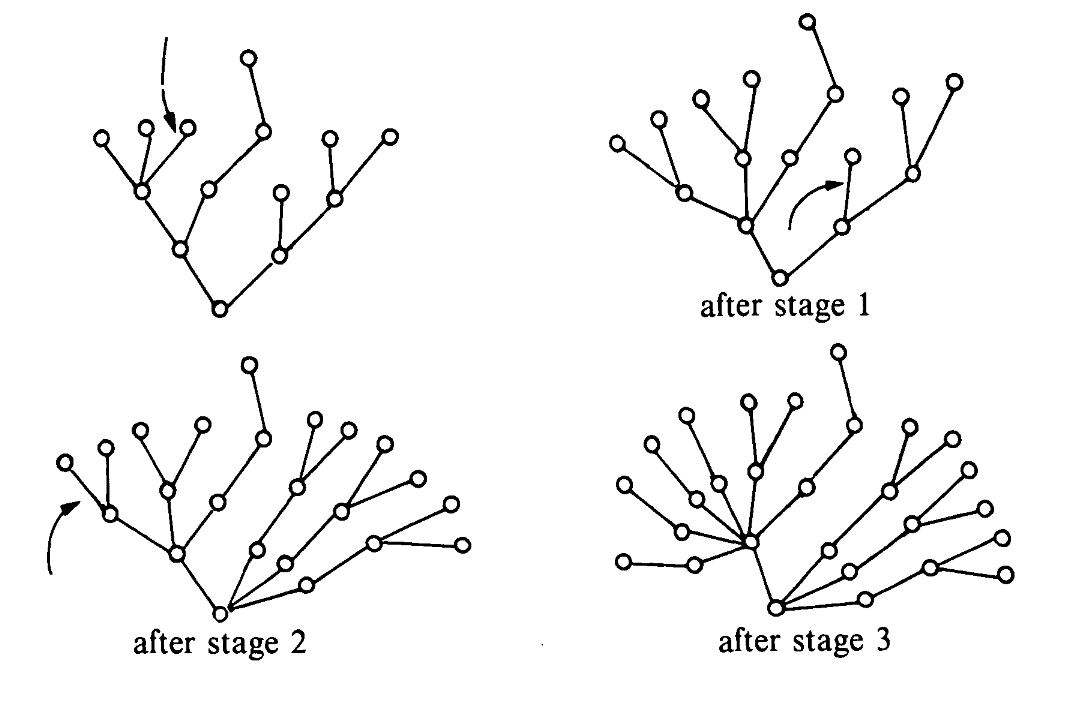
\includegraphics[width=4in]{HydraKP}
  \captionof{figure}{The first three moves of a more complicated hydra game}
\end{center}

Here, the hydra we end up with after three moves looks, to the untrained eye, to be 
significantly larger and more complicated than the one we started with, and it seems 
conceivable that we will never win this hydra game. However, we will prove the following 
somewhat surprising theorem, showing that not only can we win \emph{every} hydra game, but 
in fact we \emph{cannot lose}.

\begin{theorem}
  In every hydra game, no matter how we play, we will always win after a finite number of moves.
\end{theorem}

\begin{proof}
  We will denote runs of the hydra game by $\langle H_0, H_1, H_2, \ldots \rangle$, where 
  $H_0$ is the initial hydra that starts the game, $H_1$ is the hydra resulting after Move 1, 
  $H_2$ is the hydra resulting after Move 2, and, in general, $H_k$ is the hydra resulting after 
  Move $k$. If we ever reach an $n$ such that $H_n$ is the hydra consisting of just a root node, 
  then we have won the game, so the complete run of the game is then 
  $\langle H_0, H_1, H_2, \ldots, H_n \rangle$. We must show that every possible run of the hydra 
  game is finite.
  
  To do this, given an arbitrary hydra $H$, we will assign it an ordinal number, $\#(H)$ in 
  the following way. Starting with the terminal nodes and working our way down to the root, we 
  will assign an ordinal number to each node of the hydra. Each terminal node gets labeled with a $0$. 
  Now suppose that $u$ is a non-terminal node of $H$ and we have labeled all of the nodes 
  that are directly above $u$ (i.e., above $u$ and connected to it by an edge). Suppose that 
  there are $m$ such nodes, and they are labeled with ordinal numbers 
  $\alpha_1 \geq \alpha_2 \geq \ldots \geq \alpha_m$ (arranged in non-increasing order). Then label 
  $u$ with the ordinal 
  \[
    \omega^{\alpha_1} + \omega^{\alpha_2} + \cdots + \omega^{\alpha_m}.
  \]
  Finally, let $\#(H)$ equal the ordinal number that is assigned to the root of $H$ by this process.
  Here are a couple of simple examples to illustrate this.
  \begin{center}
    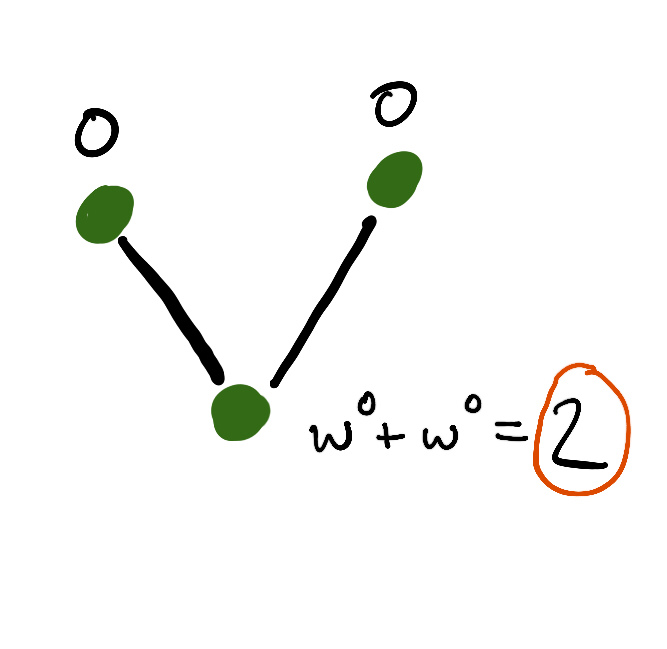
\includegraphics[width=1.5in]{Hydra9}
    \captionof{figure}{A hydra $H$ with $\#(H) = 2$}
  \end{center}
  \begin{center}
    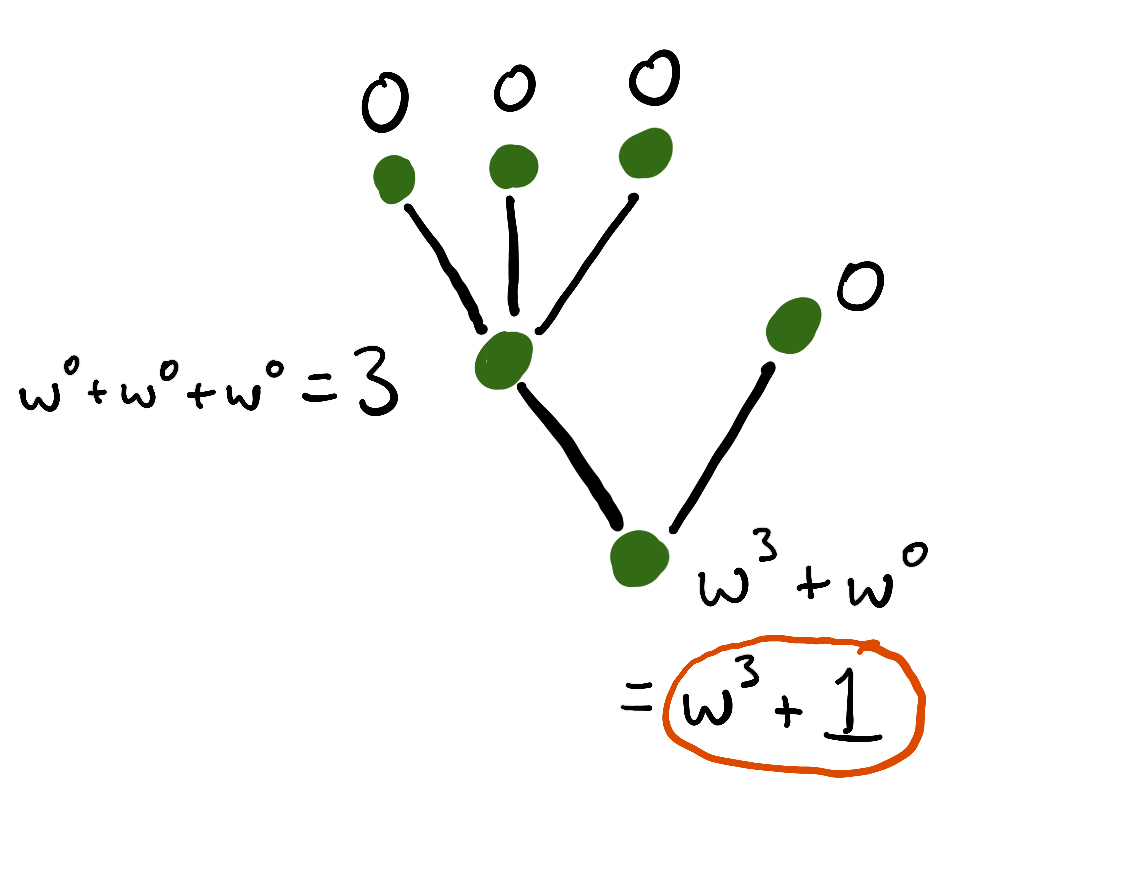
\includegraphics[width=1.5in]{Hydra10}
    \captionof{figure}{A hydra $H$ with $\#(H) = \omega^3 + 1$}
  \end{center}
  If we calculate $\#(H)$ for the first hydra presented above, we find that it is equal to 
  $\omega^{\omega^3 + 1} + 1$:
  \begin{center}
    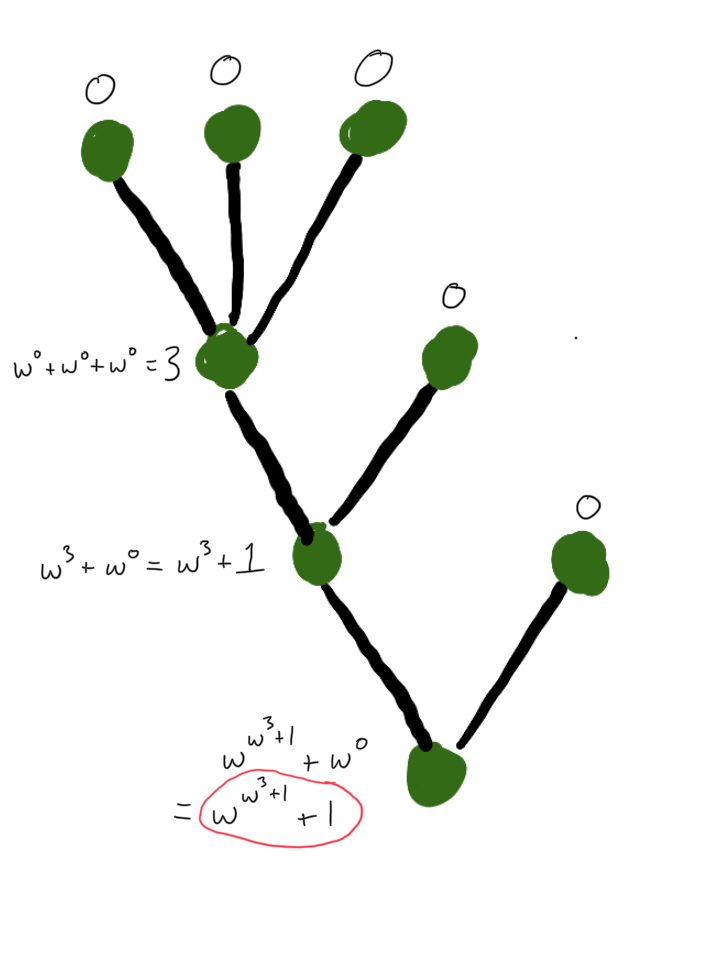
\includegraphics[width=2in]{Hydra1N}
    \captionof{figure}{A hydra $H$ with $\#(H) = \omega^{\omega^3 + 1} + 1$.}
  \end{center}
  Now let's see what happens to the ordinal number assigned to this hydra if we make a play 
  of the hydra game and chop off one of its heads. Let's suppose that we are at Move 2 and 
  chop off the left head of this hydra, as depicted in Figure 1.7 above. The resulting 
  hydra $H'$ is depicted in Figure 1.8 above, and we can calculate $\#(H')$ to be 
  $\omega^{\omega^2 \cdot 3 + 1} + 1$:
  \begin{center}
    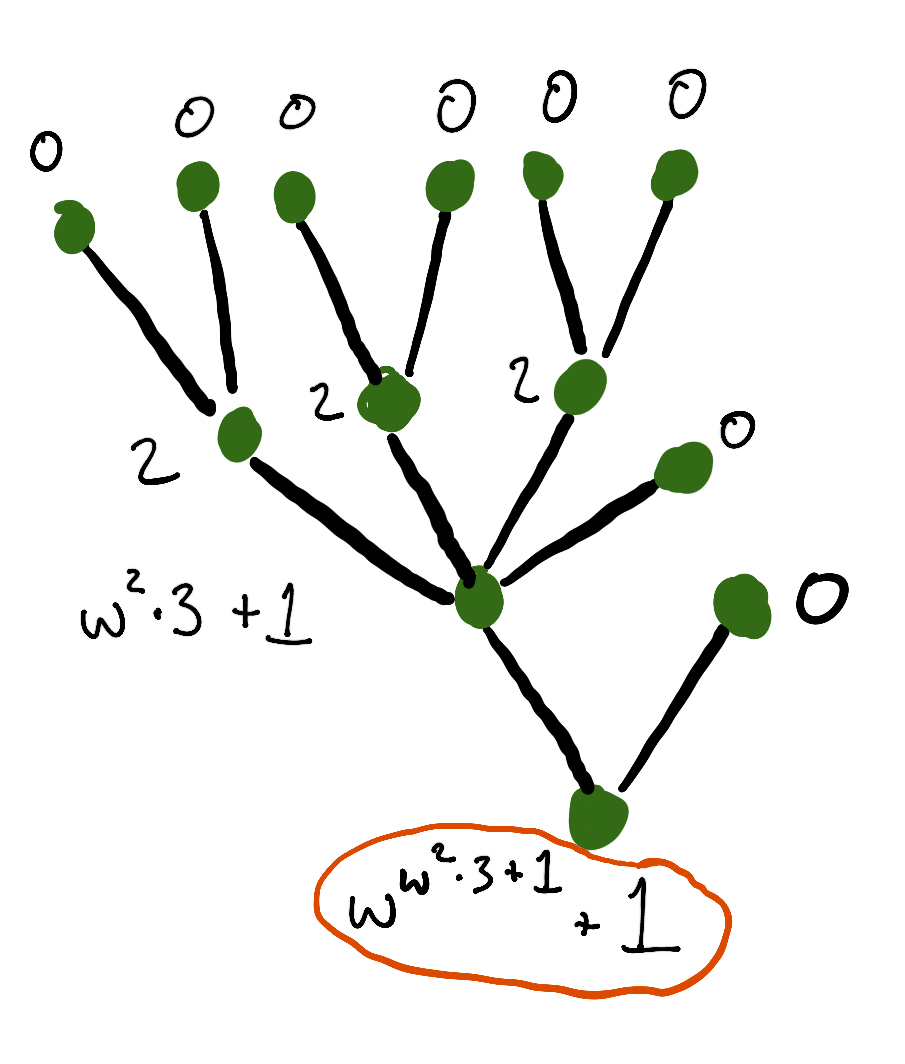
\includegraphics[width=2in]{Hydra8}
    \captionof{figure}{A hydra $H'$ with $\#(H') = \omega^{\omega^2 \cdot 3 + 1} + 1$}
  \end{center}
  
  Notice that $\omega^2 \cdot 3 < \omega^3$, so $\omega^{\omega^2 \cdot 3 + 1} + 1 < 
  \omega^{\omega^3 + 1} + 1$, i.e., $\#(H') < \#(H)$. Thus, by making a move in the hydra game and 
  chopping off a head of $H$, we created a new hydra $H'$ such that, even though $H'$ has more heads 
  than $H$, its ordinal value is strictly \emph{smaller}. This is not a coincidence.
  
  \begin{exercise}
    Calculate the ordinal numbers assigned to the hydras appearing in the run of the hydra game 
    depicted in Figure 1.9 above.
  \end{exercise}
  
  You should have found in the above exercise that the ordinal values assigned to the hydras 
  were strictly decreasing throughout the run of the game. We can in fact prove that this is 
  always the case. The following is the key step of this proof; for now, we leave it as an exercise.
  
  \begin{exercise}
    Suppose that $\langle H_0, H_1, H_2, H_3, \ldots \rangle$ is a run of the hydra game. Prove 
    that $\#(H_0) > \#(H_1) > \#(H_2) > \#(H_3) > \ldots$. In other words, performing a move in the 
    hydra game always strictly decreases the value of the ordinal assigned to the hydra. 
    (\textbf{Hint.} First prove the following basic fact about ordinal arithmetic: for every 
    ordinal $\alpha$ and every natural number $n$, we have $\omega^{\alpha} \cdot n < 
    \omega^{\alpha + 1}$.)
  \end{exercise}
  
  With the previous exercise, though, we can finish the proof of the theorem! For every run 
  of the hydra game $\langle H_0, H_1, H_2, H_3, \ldots \rangle$, we obtain a strictly decreasing 
  sequence of ordinals $\#(H_0) > \#(H_1) > \#(H_2) > \#(H_3) > \ldots$. Since the ordinals are 
  themselves well-ordered, there can be no infinite strictly decreasing sequences of ordinals. 
  Therefore, \emph{every} run of the hydra game must be finite. In other words, no matter how you 
  play the hydra game, you will always win after some finite number of moves.
\end{proof}

\section{Peano arithmetic}

Our use of infinite ordinals to prove that every hydra game must end after finitely many moves 
may seem counterintuitive and perhaps unnecessary. The theorem about hydra games is, after all, 
a statement that is entirely about finite objects. Why should we need to reason about 
infinite ordinals in order to prove it? However, a remarkable theorem of Kirby and Paris shows 
that something like this \emph{is} indeed necessary to prove the theorem. 

You may have seen before the axioms of Peano Arithmetic ($\mathsf{PA}$), introduced by Giuseppe Peano in the 
19th century. These axioms are meant to capture our intuition about the behavior of the natural numbers, 
and hence about finite discrete objects more broadly. 

The language of Peano arithmetic consists of
\begin{itemize}
  \item the equality sign $=$;
  \item a constant symbol $0$;
  \item a unary function symbol $S$.
\end{itemize}
The intended interpretation of the function $S$ is that it returns the \emph{successor} of 
its input, i.e., $S(n) = n+1$. Peano arithmetic has five axioms that are meant to describe 
the arithmetical properties of the \emph{natural numbers}. These axioms can be stated as follows:
\begin{enumerate}
  \item $0$ is a natural number.
  \item For every natural number $n$, $S(n)$ is also a natural number.
  \item For all natural numbers $m$ and $n$, if $S(m) = S(n)$, then $m = n$.
  \item For every natural number $n$, $0 \neq S(n)$, i.e., $0$ is not the successor of any 
  natural number.
  \item (Induction) If $K$ is a set such that
  \begin{itemize}
    \item $0$ is in $K$; and
    \item for every natural number $n$, if $n$ is in $K$, then $S(n)$ is also in $K$,
  \end{itemize}
  then $K$ contains every natural number.
\end{enumerate}

Peano Arithmetic captures much of our intuition about the natural numbers, and many theorems 
about the natural numbers or finite discrete objects can be proven using only $\mathsf{PA}$. For 
example, much of number theory, as well as the finite Ramsey theorem, can be established in 
$\mathsf{PA}$. However, Kirby and Paris proved that $\mathsf{PA}$ is \emph{not} strong enough 
to prove that every hydra game must end in a finite number of moves. In fact, they proved the 
following (stated in a slightly imprecise way):

\begin{theorem}[Kirby--Paris]
  If a set of axioms can prove that every hydra game must end in a finite number of moves, 
  then it can also prove the consistency of $\mathsf{PA}$.
\end{theorem}

By G\"{o}del's Second Incompleteness Theorem, $\mathsf{PA}$ cannot prove its own consistency. 
Therefore, the Kirby--Paris theorem implies that we cannot prove our theorem about hydra games 
using $\mathsf{PA}$ alone; we must use \emph{something} that goes beyond it.

\chapter{Lecture 2: Transfinite induction and recursion}

Two of the principal reasons for the centrality of well-orderings in set theory and its 
applications to other fields of mathematics are the techniques of transfinite induction 
and transfinite recursion. Let us briefly recall these techniques, in both a formal 
formulation and a more informal one that better reflects how we actually think about them in 
practice.

\section{Transfinite induction}

To motivate the statement of transfinite induction, recall classical induction on the natural numbers:

\textbf{Principle of induction:} Suppose that $P$ is a property that can hold of natural numbers and 
suppose that we know the following:
\begin{quote}
  For all $n \in \mathbb{N}$, if $P(m)$ holds for all $m < n$, then $P(n)$ holds.
\end{quote}
Then $P(n)$ holds for all $n \in \mathbb{N}$.

\medskip

A similar principle holds for arbitrary well-ordered sets, not just for $\mathbb{N}$.

\begin{theorem}[Transfinite induction] \label{thm: transfinite_induction}
  Suppose that $(X, \preceq)$ is a well-order, (or $X$ is the class of all ordinals, 
  and $\preceq$ is the usual ordering of ordinals) and suppose that $P$ is a property that can 
  hold of elements of $X$. Suppose moreover that we know the following:
  \begin{quote}
    For all $y \in X$, if $P(x)$ holds for all $x \prec y$, then $P(y)$ holds.
  \end{quote}
  Then $P(y)$ holds for all $y \in X$.
\end{theorem}

As a simple illustration, let us prove that ordinal addition is associative.

\begin{theorem}
  For all ordinals $\alpha,\beta,\gamma$, we have $(\alpha + \beta) + \gamma = \alpha + (\beta + \gamma)$.
\end{theorem}

\begin{proof}
  The proof is by induction on $\gamma$. Thus, fix ordinals $\alpha$ and $\beta$. We will prove 
  the following:
  \begin{quote}
    For every ordinal $\gamma$, if $(\alpha + \beta) + \varepsilon = \alpha + (\beta + \varepsilon)$ 
    for all $\varepsilon < \gamma$, then $(\alpha + \beta) + \gamma = \alpha + (\beta + \gamma)$.
  \end{quote}
  Theorem \ref{thm: transfinite_induction} will them imply that $(\alpha + \beta) + \gamma = 
  \alpha + (\beta + \gamma)$ for all ordinals $\gamma$. 
  
  To this end, fix an ordinal $\gamma$, and suppose that $(\alpha + \beta) + \varepsilon = 
  \alpha + (\beta + \varepsilon)$ for all $\varepsilon < \gamma$. We must show that 
  $(\alpha + \beta) + \gamma = \alpha + (\beta + \gamma)$. The proof splits into three cases, 
  based on whether $\gamma = 0$, $\gamma$ is a successor ordinal, or $\gamma$ is a nonzero 
  limit ordinal.
  
  \textbf{Case 1: $\gamma = 0$.} Recall that, for any ordinal $\delta$, we have $\delta + 0 = \delta$. 
  Thus, we have
  \[
    (\alpha + \beta) + 0 = \alpha + \beta = \alpha + (\beta + 0),
  \]
  as desired.
  
  \textbf{Case 2: $\gamma$ is a successor ordinal.} Let $\varepsilon$ be such that 
  $\gamma = \varepsilon + 1$. Recall that, by definition of ordinal addition, we know that, 
  for all ordinals $\delta$, we have $\delta + (\varepsilon + 1) = (\delta + \varepsilon) + 1$. Then
  \begin{align*}
    (\alpha + \beta) + \gamma &= (\alpha + \beta) + (\varepsilon + 1) \\ 
    &= ((\alpha + \beta) + \varepsilon) + 1 \\ 
    &= (\alpha + (\beta + \varepsilon)) + 1 \\ 
    &= \alpha + ((\beta + \varepsilon) + 1) \\ 
    &= \alpha + (\beta + (\varepsilon + 1)) \\ 
    &= \alpha + (\beta + \gamma),
  \end{align*}
  where the equality between lines 2 and 3 follow from the inductive hypothesis and all other equalities 
  follow from the definition of ordinal addition.
  
  \textbf{Case 3: $\gamma$ is a nonzero limit ordinal.} In this case recall that, by the definition 
  of ordinal addition, for every ordinal $\delta$,
  \[
    \delta + \gamma = \sup\{\delta + \varepsilon \mid \varepsilon < \gamma\}.
  \]
  Now we have
  \begin{align*}
    (\alpha + \beta) + \gamma &= \sup\{(\alpha + \beta) + \varepsilon \mid \varepsilon < \gamma\} \\ 
    &= \sup\{\alpha + (\beta + \varepsilon) \mid \varepsilon < \gamma\} \\ 
    &= \alpha + \sup\{\beta + \varepsilon \mid \varepsilon < \gamma\} \\ 
    &= \alpha + (\beta + \gamma), 
  \end{align*}
  where the equality between lines 1 and 2 follows from the inductive hypothesis and all other 
  equalities follow from the definition of ordinal arithmetic.
  
  This completes all three cases and thus the proof of the theorem.
\end{proof}

Another example of a proof by transfinite induction involves \emph{strictly increasing functions}.

\begin{definition}
  Suppose that $(A, \leq_A)$ and $(B, \leq_B)$ are two well-orders. Then a function 
  $f:A \ra B$ is said to be \emph{strictly increasing} if, for all $x,y \in A$, we have
  \[
    (x <_A y) \Longrightarrow (f(x) <_B f(y)).
  \]
\end{definition}

\begin{exercise}
  Suppose that $(A, \leq_A)$ is a well-order and $f:A \ra A$ is strictly increasing. Prove 
  that $x \leq f(x)$ for all $x \in A$.
\end{exercise}

\section{Transfinite recursion}

You are probably familiar with the notion of a \emph{sequence} indexed by the natural numbers. 
For example, the sequence $\langle 1/2^n \mid n < \omega \rangle$ is the 
sequence $\langle 1, 1/2, 1/4, 1/8, \ldots \rangle$. But we can equally well have sequences 
indexed by other ordinal numbers.

\begin{definition}
  Let $\alpha$ be an ordinal. An \emph{$\alpha$-sequence} is a sequence of the form 
  $\langle x_\eta \mid \eta < \alpha \rangle$, i.e., a sequence that is indexed by 
  the set of ordinals less than $\eta$.
\end{definition}

Roughly speaking, a construction of a sequence by \emph{recursion} is a construction done 
by specifying one element at a time, with the choice of a particular element possibly depending on 
the initial segment of the sequence that has been constructed so far. For example, the 
$\omega$-sequence $\langle 1/2^n \mid n < \omega \rangle$ can be given a recursive definition 
as follows:
\begin{itemize}
  \item $x_0 = 1$;
  \item for all $n < \omega$, $x_{n+1} = x_n/2$.
\end{itemize}

In general, it is not hard to see that, if one is given a rule for selecting $x_0$ and, given 
$x_n$, a rule for selecting $x_{n+1}$, then there is exactly one sequence $\langle x_n \mid n 
< \omega \rangle$ that satisfies these rules.

Another well-known recursively defined sequence is the \emph{Fibonacci} sequence, 
$\langle 0, 1, 1, 2, 3, 5, 8, 13, \ldots \rangle$, defined recursively as follows:
\begin{itemize}
  \item $x_0 = 0$;
  \item $x_1 = 1$;
  \item for all $n < \omega$, $x_{n+2} = x_n + x_{n+1}$.
\end{itemize}

Just as with induction, recursion can be extended to arbitrary well-orders. 

\begin{theorem}[Transfinite recursion] \label{thm: transfinite_recursion}
  Suppose that $\alpha$ is an ordinal and $Z$ is a nonempty set. Let $\mathcal{S}$ be the set of all 
  sequences of elements of $Z$ of length less than $\alpha$, and suppose that 
  $F: \mathcal{S} \rightarrow Z$ is a function. Then there is a unique sequence 
  $\langle x_\eta \mid \eta < \alpha \rangle$ such that, for all $\xi < \alpha$, we have
  \[
    x_\xi = F(\langle x_\eta \mid \eta < \xi \rangle).
  \]
\end{theorem}

Informally speaking, Theorem \ref{thm: transfinite_recursion} is saying that one can construct 
sequences by (arbitrarily long) transfinite recursion. In applications of the theorem, one is 
typically seeking to construct an $\alpha$-sequence for some ordinal $\alpha$. The function 
$F$ in the theorem is describing a rule that tells you how to pick the \emph{next} element of 
the sequence given what has come so far. The theorem then says that there is exactly one 
sequence that satisfies all of these rules.

We have in fact already seen recursive constructions; the rigorous definitions of ordinal 
arithmetic given in Chapter 1 were definitions by transfinite recursion.

In practice, when applying transfinite recursion, we typically want to produce an $\alpha$-sequence 
$\langle x_\eta \mid \eta < \alpha \rangle$ of elements of a set $Z$ such that the sequence 
satisfies certain desired properties. The construction of such a sequence will typically 
consist of the following two steps:
\begin{enumerate}
  \item For $\xi < \alpha$, describe a rule for choosing $x_\xi$ based on the sequence 
  $\langle x_\eta \mid \eta < \xi \rangle$ constructed so far. Sometimes this rule will 
  break into cases depending on whether $\xi$ is $0$, a successor ordinal, or a nonzero 
  limit ordinal, though sometimes these distinctions will not matter.
  \item Show that a sequence constructed according to this rule will have the desired properties.
\end{enumerate}

\section{Well-ordering principle}

Transfinite induction and transfinite recursion gain additional power when paired with the 
well-ordering principle, which can be stated as follows.

\begin{theorem}[Well-ordering principle]
  For every set $X$, there is a binary relation $\preceq$ on $X$ such that $(X, \preceq)$ is a 
  well-order.
\end{theorem}

We have stated the well-ordering principle as a theorem, and it is indeed a theorem of 
$\mathsf{ZFC}$. Over the axioms of $\mathsf{ZF}$ (which are just the axioms of $\mathsf{ZFC}$ 
without the axiom of choice), it turns out that the well-ordering principle is 
\emph{equivalent} to the axiom of choice, so one could just as well think of it as 
an alternative formulation of the axiom of choice.

Since the ordinal numbers are themselves well-ordered, we know that, for every 
\emph{cardinal} number $\kappa$, there is a \emph{minimal} ordinal of cardinality 
$\kappa$. In practice, we identify the cardinal $\kappa$ with this ordinal, which we 
will also refer to as $\kappa$. A key property of this ordinal $\kappa$ is the following:
\begin{quote}
  Every proper initial segment of $\kappa$ has cardinality strictly less than $\kappa$.
\end{quote}
This is useful enough in practice that it is worth it to state a more refined version of 
the well-ordering principle.

\begin{theorem}[Well-ordering principle, version 2]
  Suppose that $X$ is a set and $\kappa = |X|$. Then there is a sequence $\vec{x} = \langle x_\alpha 
  \mid \alpha < \kappa \rangle$ such that
  \begin{itemize}
    \item $X = \{x_\alpha \mid \alpha < \kappa\}$; and
    \item $\vec{x}$ is injective, i.e., for all $\alpha < \beta < \kappa$, we have $x_\alpha 
    \neq x_\beta$.
  \end{itemize}
\end{theorem}

\section{Applications of transfinite recursion to Euclidean space}

In this section, we apply the tools of transfinite recursion to construct interesting objects in 
Euclidean space, focusing in particular on $\bb{R}^2$ and $\bb{R}^3$. This will involve transfinite 
recursions of length $|\bb{R}|$. We denote the cardinality of $\bb{R}$ by $\mathfrak{c}$; sometimes 
this cardinal is simply referred to as ``the continuum". As you may know, the precise value of 
$\mathfrak{c}$ is not determined by the axioms of $\mathsf{ZFC}$. It could be $\aleph_1$, $\aleph_2$, or 
more generally any cardinal $\kappa$ such that the cofinality of $\kappa$ is uncountable. 
Note that 
\[
  \mathfrak{c} = |\mathbb{R}| = |\mathbb{R}^2| = |\mathbb{R}^3| = \ldots = |\mathbb{R}^\omega|.
\]

Our first example, due to Mazurkiewicz, establishes the existence of a so-called \emph{two-point set}.

\begin{theorem} \label{thm: two_point_set}
  There is a subset $A$ of $\bb{R}^2$ such that every straight line in $\bb{R}^2$ intersects 
  $A$ in exactly two points.
\end{theorem}

\begin{proof}
  Let $\mathcal{L}$ be the set of all lines in $\bb{R}^2$. We first claim that $|\mc{L}| = \mathfrak{c}$.
  Here's one way to see that. First, there are \emph{at least} $\mathfrak{c}$-many lines, since, for 
  example, for every real number $r$, the equation $y = r$ describes a unique horizontal line in 
  $\mathbb{R}^2$. Thus, $|\mc{L}| \geq \mathfrak{c}$. On the other hand, to see that 
  $|\mc{L}| \leq \mathfrak{c}$, note that, to specify a line in $\bb{R}^2$, it suffices to specify 
  two distinct points on the line. There are only $\mathfrak{c} \times \mathfrak{c} = \mathfrak{c}$-many 
  ways of choosing two points in $\bb{R}^2$. Thus, $|\mathcal{L}| \leq \mathfrak{c}$.
  
  Using the well-ordering principle, we can fix an injective sequence $\langle \ell_\alpha \mid 
  \alpha < \mathfrak{c} \rangle$ of lines in $\bb{R}^2$ such that every element of $\mc{L}$ is equal 
  to $\ell_\alpha$ for some $\alpha < \mathfrak{c}$. We will recursively construct a sequence 
  $\langle A_\alpha \mid \alpha < \mathfrak{c} \rangle$ satisfying the recursion requirements 
  that, for every $\beta < \mathfrak{c}$:
  \begin{enumerate}
    \item $A_\beta$ is a subset of $\bb{R}^2$ of size at most 2;
    \item $\bigcup_{\alpha \leq \beta} A_\alpha$ does not contain any three points that lie on the 
    same line;
    \item $\bigcup_{\alpha \leq \beta} A_\alpha$ contains exactly two points on the line 
    $\ell_\beta$.
  \end{enumerate}
  If we can succeed in this construction, then the set $A = \bigcup_{\alpha < \mathfrak{c}} A_\alpha$ 
  will be as required by the theorem. Let us now describe the recursive construction.
  
  Fix an ordinal $\beta < \mathfrak{c}$ and suppose that we have constructed 
  $\langle A_\alpha \mid \alpha < \beta \rangle$ that satisfies the recursion requirements so far.
  The following describes how to choose a set $A_\beta$ to continue the construction.
  
  Let $B = \bigcup_{\alpha < \beta} A_\alpha$, i.e., $B$ is the set of points that we have chosen 
  so far. Let $\mathcal{G}$ be the set of all lines passing through two points of $B$. Note 
  that 
  \[ 
    |\mathcal{G}| \leq |B| \times |B| \leq |\beta| \times |\beta| < \mathfrak{c}.
  \]
  When choosing $A_\beta$, we must be careful not to add any new points that are on lines in 
  $\mathcal{G}$ to satisfy requirement (2) above.
  
  Consider the line $\ell_\beta$. We must make sure that $\bigcup_{\alpha \leq \beta} A_\beta$ 
  contains exactly two points on $\ell_\beta$ to satisfy requirement (3) above. 
  If $B$ already contains two points from $\ell_\beta$, then we can simply let $A_\beta = \emptyset$ 
  and move on to the next step. If $B$ contains either 0 or 1 points from $\ell_\beta$, then notice 
  that $\ell_\beta \notin \mathcal{G}$, and therefore every line in $\mathcal{G}$ intersects 
  $\ell_\beta$ in at most one point. Since $|\mathcal{G}| < \mathfrak{c}$ and the number of points 
  on $\ell_\beta$ is exactly $\mathfrak{c}$, we know that $|\ell_\beta \setminus \bigcup 
  \mathcal{G}| = \mathcal{c}$, i.e., there are $\mathfrak{c}$-many points on $\ell_\beta$ that 
  are not on any of the lines in $\mathcal{G}$. 
  
  If $B$ contains 0 points from $\ell_\beta$, then let $A_\beta$ consist of precisely 2 points 
  from $\ell_\beta \setminus \bigcup \mathcal{G}$, and if $B$ contains 1 point from $\ell_\beta$, 
  then let $A_\beta$ consist of precisely 1 point from $\ell_\beta \setminus \bigcup \mathcal{G}$. 
  This completes the description of stage $\beta$ of the construction; one can check that we have 
  maintained the recursion requirements (1) -- (3). Thus, this completes the construction and 
  the proof of the theorem.
\end{proof}

The next results concern ``circles" in Euclidean space. These are probably what you intuitively 
expect them to be. By ``circle" we mean the boundary of the circle, not its interior. We consider 
only nontrivial circles, i.e., circles whose radius is strictly positive. In 
$\mathbb{R}^2$, one can specify a circle by fixing real numbers $x_0$ and $y_0$ and a radius 
$r > 0$; the circle is then the set of all points $(x,y) \in \bb{R}^2$ such that 
$(x-x_0)^2 + (y - y_0)^2 = r^2$. One can do something similar, but more complicated, in 
$\bb{R}^3$: one can specify a circle by first specifying a plane in $\bb{R}^3$ and then specifying 
a circle in that plane in the same way as we did in $\bb{R}^2$. However, for what we want to 
discuss here, these formal descriptions are not necessary and may even get in the way of intuition. 
The two basic facts we will need about circles are the following:

\begin{fact}
  Suppose that $a$, $b$, and $c$ are any three points in $\bb{R}^2$ or $\bb{R}^3$ that are not 
  all on the same line. Then there is a unique circle that contains all three points.
\end{fact}

\begin{fact}
  If $C_0$ and $C_1$ are two distinct circles in $\bb{R}^2$ or $\bb{R}^3$, then $C_0$ and $C_1$ 
  intersect in at most two points.
\end{fact}

First, we have an exercise giving a variant on Theorem \ref{thm: two_point_set}.

\begin{exercise}
  There is a subset $A$ of $\mathbb{R}^2$ such that every circle in $\bb{R}^2$ intersects $A$ in 
  exactly three points.
\end{exercise}

The next example concerns covering Euclidean space by pairwise disjoint circles. Let us say 
precisely what we mean by this. If $\mc{C}$ is a set of circles (in either $\bb{R}^2$ or 
$\bb{R}^3$), then we say that $\mc{C}$ is \emph{pairwise disjoint} if, for all distinct 
$C_0, C_1 \in \mathcal{C}$, we have $C_0 \cap C_1 = \emptyset$. In other words, 
$\mc{C}$ is pairwise disjoint if no two distinct element of $\mc{C}$ intersect each other.

We say that a pairwise disjoint set $\mc{C}$ of circles \emph{covers} $\bb{R}^2$ (or $\bb{R}^3$) 
if every element of $\bb{R}^2$ (or $\bb{R}^3$) is in an element of $\mc{C}$. In other words, 
$\mc{C}$ covers $\bb{R}^2$ (or $\bb{R}^3$) if $\bigcup \mc{C} = \bb{R}^2$ (or 
$\bigcup \mc{C} = \bb{R}^3)$. Note that, since $\mc{C}$ is pairwise disjoint, if 
$\mc{C}$ covers $\bb{R}^2$ or $\bb{R}^3$, then every point is in \emph{exactly} one element of 
$\mc{C}$. 

We are interested in the question of whether Euclidean spaces can be covered by pairwise disjoint sets of 
circles and, if they can, what further requirements we can place on these circles. We first show that 
this is impossible for $\bb{R}^2$.

\begin{theorem}
  $\bb{R}^2$ cannot be covered by a pairwise disjoint set of circles.
\end{theorem}

\begin{proof}
  The key observation about $\bb{R}^2$ is the following: every circle in $\bb{R}^2$ divides the 
  rest of the plane into a region \emph{inside} the circle and a region outside the circle. If 
  $C_0$ is a circle and $a$ is a point 
  \emph{inside} of $C_0$, then any circle $C_1$ containing $a$ that is disjoint from $C_0$ must 
  itself lie entirely inside of $C_1$ (see picture below).
  \begin{center}
    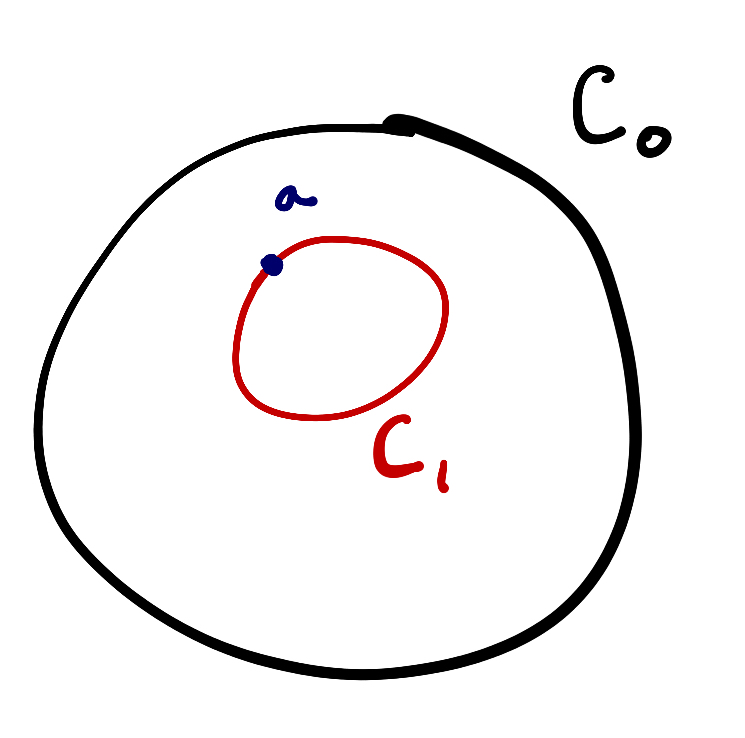
\includegraphics[width=2in]{nesting_circles}
  \end{center}
  Now suppose for the sake of contradiction that $\mc{C}$ is a pairwise disjoint set of circles 
  that covers $\bb{R}^2$. Simultaneously recursively define sequences $\langle C_n \mid n < \omega 
  \rangle$ and $\langle a_n \mid n < \omega \rangle$ as follows:
  \begin{itemize}
    \item $C_0$ is an arbitrary element of $\mc{C}$;
    \item for each $n < \omega$, $a_n$ is the \emph{center} of the circle $C_n$;
    \item for each $n < \omega$, $C_{n+1}$ is the unique element of $\mc{C}$ that passes through 
    $a_n$.
  \end{itemize}
  In other words, $C_0$ is an arbitrary element of $\mc{C}$, $C_1$ is the unique element of $\mc{C}$ 
  that passes through the center of $C_0$, $C_2$ is the unique element of $\mc{C}$ that passes 
  through the center of $C_1$, and so on. By the observation above, for each $n < \omega$, the circle 
  $C_{n+1}$ lies entirely inside of $C_n$. Moreover, since $C_{n+1}$ passes through the \emph{center} 
  of $C_n$, the radius of $C_{n+1}$ must be less than half the radius of $C_n$. For all 
  $n < \omega$, let $r_n$ denote the radius of $C_n$. We have shown that 
  \[
    r_{n+1} < \mathfrak{r_n}{2}
  \]
  for all $n$, and hence the radii $\langle r_n \mid n < \omega \rangle$ converge to $0$. 
  Therefore, the centers $\langle a_n \mid n < \omega \rangle$ of the circles 
  $\langle C_n \mid n < \omega \rangle$ converge to a single limit point; call this limit point 
  $b$.
  \begin{center}
    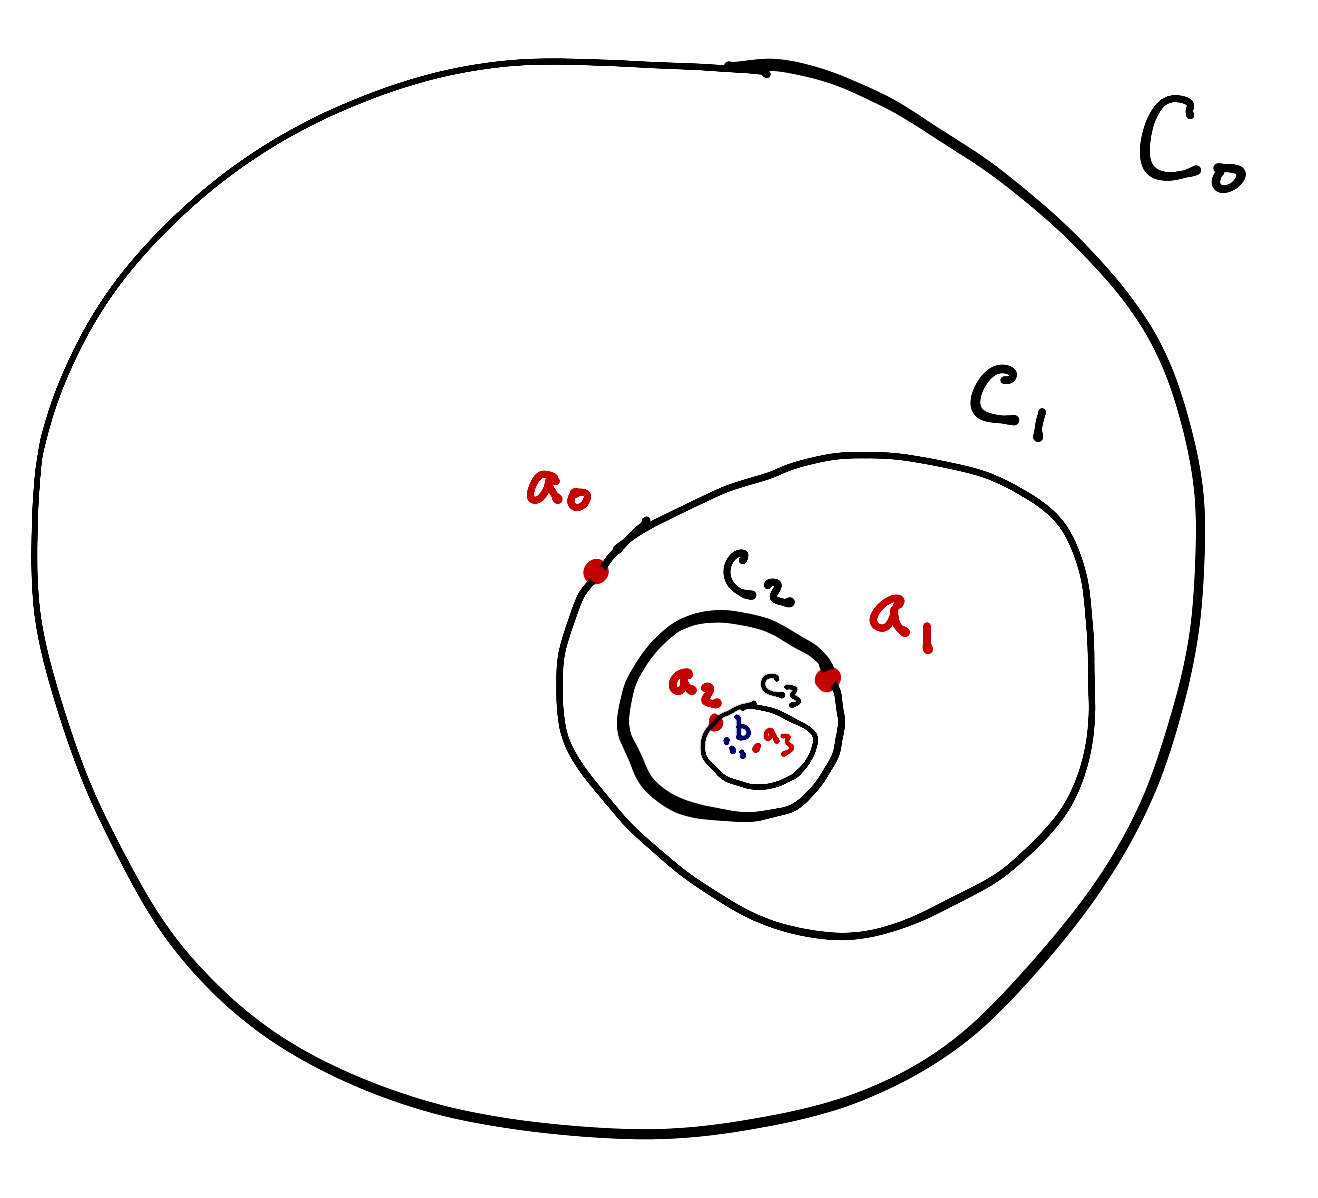
\includegraphics[width=3.5in]{nesting-limit}
    \captionof{figure}{The centers $\langle a_n \mid n < \omega \rangle$ of the circles converging 
    to a limit point $b$.}
  \end{center}
  Notice that $b$ must lie on the \emph{inside} of $C_n$ for every $n < \omega$. 
  
  We are assuming that $\mc{C}$ covers $\bb{R}^2$. We can therefore find a circle 
  $C^* \in \mc{C}$ such that $b \in C^*$. Since $b$ is \emph{inside} $C_n$ for all $n < \omega$, 
  we know that $C^*$ cannot be equal to $C_n$ for any $n < \omega$. Let $r^*$ be the radius of $C^*$. Since 
  the radii $\langle r_n \mid n < \omega \rangle$ converge to $0$, we can fix an 
  $n < \omega$ such that $r_n < r^*$. But now we know the following two things:
  \begin{enumerate}
    \item $C^*$ contains a point on the inside of $C_n$, namely $b$.
    \item The radius of $C^*$, $r^*$, is larger than the radius of $C_n$, $r_n$. Therefore, 
    $C^*$ cannot be entirely contained in the inside of $C_n$.
  \end{enumerate}
  It follows from the two items above that $C^*$ contains points both inside and outside $C_n$ 
  and therefore it must intersect $C_n$:
  \begin{center}
    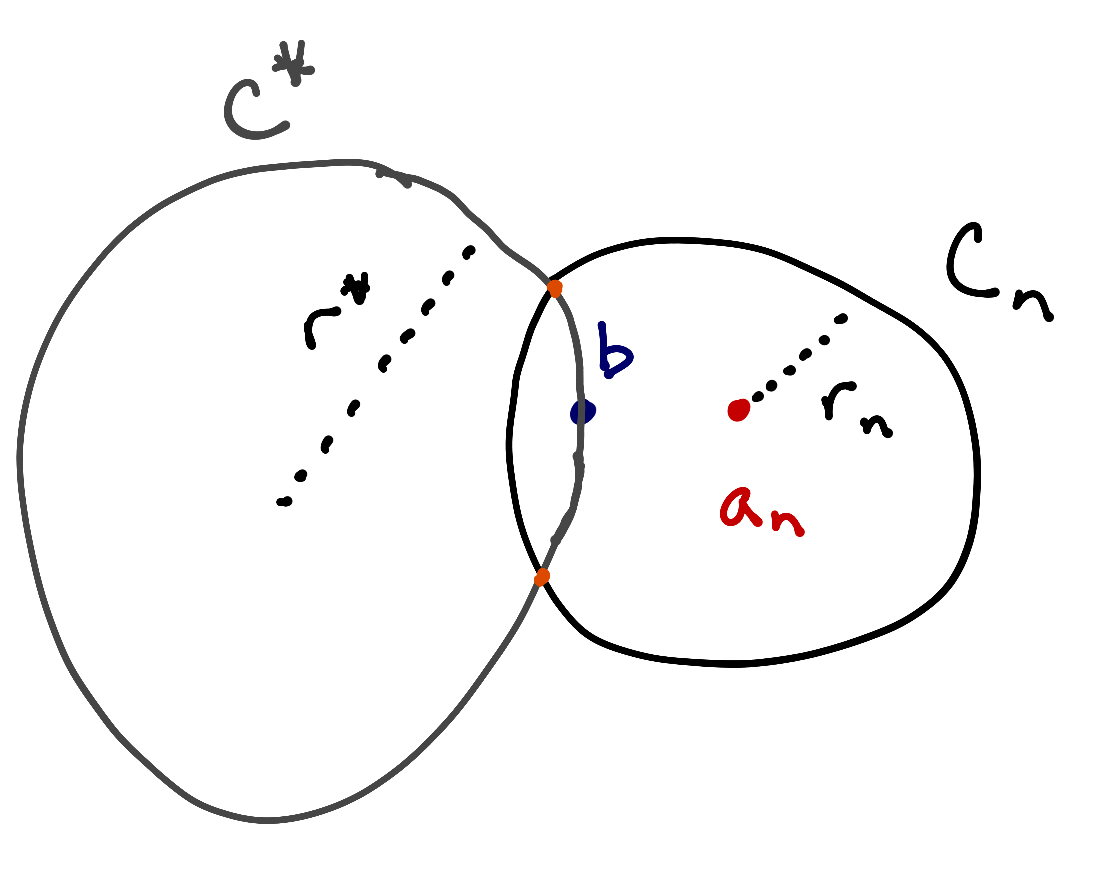
\includegraphics[width=3in]{intersecting-circles}
    \captionof{figure}{$C^*$ contains points both inside and outside $C_n$, so they 
    must intersect.}
  \end{center}
  However, $C^*$ and $C_n$ are distinct elements of $\mathcal{C}$, which was supposed to be a pairwise 
  disjoint family. This is a contradiction, thus proving the theorem.
\end{proof}

However, perhaps surprising, we now show that $\bb{R}^3$ \emph{can} be covered by a pairwise 
disjoint set of circles. The key difference between $\bb{R}^3$ and $\bb{R}^2$ with respect to 
this problem is that, in $\bb{R}^3$, unlike in $\bb{R}^2$, a circle no longer divides the 
rest of the space into ``inside" and ``outside", and this gives us much more freedom to construct 
interesting sets of circles. For instance, we can have two disjoint circles that are \emph{linked}, 
like successive rings in a chain.

We will prove, in fact, not only that $\bb{R}^3$ can be covered by a pairwise disjoint set of circles, 
but that all of the circles in this set can be required to have any specified radius (we will 
construct such a set containing only circles of radius $1$). 

\begin{theorem}
  There is a pairwise disjoint family $\mc{C}$ of circles in $\bb{R}^3$ such that
  \begin{enumerate}
    \item every circle in $\mc{C}$ has radius $1$; and
    \item $\mc{C}$ covers $\bb{R}^3$.
  \end{enumerate}
\end{theorem}

\begin{proof}
  Let $\langle a_\alpha \mid \alpha < \mathfrak{c} \rangle$ be an injective sequence of points 
  in $\bb{R}^3$ such that every point in $\bb{R}^3$ is equal to $a_\alpha$ for some $\alpha < \mathfrak{c}$.
  
  We will recursive construct a sequence $\langle C_\alpha \mid \alpha < \mathfrak{c} \rangle$ satisfying 
  the recursion requirements that, for every $\beta < \mathfrak{c}$:
  \begin{enumerate}
    \item $C_\beta$ is either the empty set or a circle in $\bb{R}^3$ of radius $1$;
    \item for all $\alpha < \beta$, we have $C_\alpha \cap C_\beta = \emptyset$;
    \item $a_\beta \in \bigcup_{\alpha \leq \beta} C_\beta$.
  \end{enumerate}
  If we can succeed in this construction, then the set
  \[
    \mc{C} = \{C_\alpha \mid \alpha < \mathfrak{c} \text{ and } C_\alpha \text{ is a circle in } \bb{R}^3\}
  \]
  is as required the theorem. Let us now describe the recursive construction.
  
  Fix an ordinal $\beta < \mathfrak{c}$ and suppose that we have constructed 
  $\langle C_\alpha \mid \alpha < \beta \rangle$ that satisfies the recursion requirements so far. 
  The following describes how to choose $C_\beta$ to continue the construction.
  
  Consider the point $a_\beta$. If there is $\alpha < \beta$ such that $a_\beta \in C_\alpha$, 
  then we can simply let $C_\beta = \emptyset$ and move on to the next step. Otherwise, to satisfy 
  requirements (1) and (3), we need to choose $C_\beta$ to be a circle in $\bb{R}^3$ of radius $1$ 
  that passes through $x_\beta$. To satisfy requirement (2), we must make sure that $C_\beta$ 
  is disjoint from $C_\alpha$ for all $\alpha < \beta$.
  
  Let $\mathcal{B} = \{C_\alpha \mid \alpha < \beta \text{ and } C_\alpha \neq \emptyset\}$. 
  In other words, $\mathcal{B}$ is the set of all circles chosen so far. Note that, for each 
  $C_\alpha \in \mc{B}$, there is a unique plane $P_\alpha$ containing $C_\alpha$. Moreover, 
  there are precisely $\mathfrak{c}$-many planes that pass through the point $a_\beta$. 
  Therefore, since $|\mathcal{B}| \leq |\beta| < \mathfrak{c}$, we can find a plane 
  $P^*$ passing through $a_\beta$ such that, for every $C_\alpha \in \mathcal{B}$, 
  $P^*$ does not contain $C_\alpha$.
  
  Now note that, if $P$ is a plane and $C$ is a circle that is not contained in $P$, then 
  $C$ intersects $P$ in at most two points. Let $Q = \bigcup_{\alpha < \beta} P^* \cap C_\alpha$, 
  i.e., $Q$ is the set of points in $P^*$ that are in $C_\alpha$ for some $\alpha < \beta$. 
  By the previous paragraph, $P^* \cap C_\alpha$ has size at most two for every $\alpha < \beta$. 
  Therefore, we have $|Q| \leq |\beta| \times 2 < \mathfrak{c}$.
  
  Let $\mc{D}$ be the set of circles $C$ such that
  \begin{itemize}
    \item $C$ passes through $a_\beta$;
    \item $C$ is contained in $P^*$;
    \item $C$ has radius 1.
  \end{itemize}
  
  We would like to choose an element of $\mc{D}$ to be our circle $C_\beta$. 
  The following is left as an exercise:
  
  \begin{exercise}
    $|\mc{D}| = \mathfrak{c}$.
  \end{exercise}
  
  We need to require that $C_\beta$ is disjoint from $C_\alpha$ for all $\alpha < \beta$. 
  Since we are going to choose $C_\beta$ to be contained in $P^*$, this amounts to choosing 
  $C_\beta$ so that it is disjoint from $Q$.
  Let us call a circle $C \in \mc{D}$ \emph{bad} if $C \cap Q \neq \emptyset$. Let $\mc{D}^-$ 
  be the set of bad elements of $\mc{D}$. For each $C \in \mc{D}^-$, choose 
  $q_C \in C \cap Q$. 
  
  Our goal is to show that $\mc{D} \setminus \mc{D}^- \neq \emptyset$. The following is also left as 
  an exercise:
  
  \begin{exercise}
    If $u$ and $v$ are two distinct points in a plane $P$, then there are at most two circles 
    that are contained in $P$, pass through both $u$ and $v$, and have radius $1$.
  \end{exercise}
  
  By the exercise, for each $q \in Q$, there are at most \emph{two} circles $C \in \mc{D}^-$ such 
  that $q_C = q$. Since $|Q| < \mathfrak{c}$, it follows that 
  \[
    |\mc{D}^-| \leq |Q| \times 2 < \mathfrak{c}.
  \]
  Since $|\mc{D}| = \mathfrak{c}$, we know that $\mc{D}$ contains circles that are not bad, so 
  we can choose $C_\beta$ to be any element of $\mc{D}$ that is not bad. This completes stage 
  $\beta$ of the construction. By our construction, we know that
  that:
  \begin{itemize}
    \item $C_\beta$ is a circle of radius $1$ passing through $a_\beta$;
    \item $C_\beta \cap C_\alpha = \emptyset$ for all $\alpha < \beta$,
  \end{itemize}
  so we have maintained the recursion requirements. This completes the construction of 
  $\mc{C}$ and hence the proof of the theorem.
\end{proof}

\chapter{Lecture 3: The axiom of choice and its consequences}

The axiom of choice is an incredibly important, useful, and sometimes controversial 
axiom in set theory. It forms the ``$\mathsf{C}$" in ``$\mathsf{ZFC}$", which are the 
standard axioms of set theory. (The ``$\mathsf{Z}$" and  ``$\mathsf{F}$" stand for ``Zermelo" 
and ``Fraenkel", respectively. ``$\mathsf{ZF}$" denotes the axioms of $\mathsf{ZFC}$ without 
the axiom of choice.) In this lecture, we review the axiom of choice and its equivalent 
formulations and present a couple basic applications thereof.

\section{The axiom of choice}

Roughly speaking, the axiom of choice asserts that, given any collection of nonempty sets, 
one can form a new collection by choosing one element from each set. More formally, it can be 
formulated as follows.

\begin{definition}[Axiom of choice]
  The \emph{axiom of choice} is the following assertion: Whenever $I$ is a set and 
  $\langle X_i \mid i \in I \rangle$ is such that each $X_i$ is a nonempty set, there is 
  a sequence $\langle y_i \mid i \in I \rangle$ such that, for all $i \in I$, we have 
  $y_i \in X_i$.
\end{definition}

The axiom of choice can also be phrased in terms of functions:
\begin{quote}
  Whenever $I$ is a set and $F$ is a function with domain $I$ such that $F(i)$ is a nonempty set 
  for all $i \in I$, there is a function $g$ with domain $I$ such that $g(i) \in F(i)$ for all 
  $i \in I$.
\end{quote}

As we shall see, the axiom of choice is incredibly powerful and is essential to proving a number 
of important theorems. It can also lead to some counterintuitive consequences, which has led 
to it being somewhat controversial. Let us note now, though, that, due to a theorem of 
G\"{o}del, there is no cost in consistency strength in assuming the axiom of choice.

\begin{theorem}[G\"{o}del]
  If the axioms of $\mathsf{ZF}$ are consistent, then so are the axioms of $\mathsf{ZFC}$.
\end{theorem}

(We refer the reader to any standard set theory textbook for a precise statement of the axioms 
of $\mathsf{ZFC}$.)

There are a number of statements that are equivalent to the axiom of choice over $\mathsf{ZF}$; 
we mention here two especially important ones. In fact, we have already seen one of them: the 
well-ordering principle, which states that every set can be well-ordered:

\begin{definition}[Well-ordering principle]
  The \emph{well-ordering principle} is the following assertion: Whenever $X$ is a set, there is 
  a binary relation $\preceq$ on $X$ such that $(X, \preceq)$ is a well-order.
\end{definition}

The second important statement that is equivalent to the axiom of choice is known as 
\emph{Zorn's lemma}. To state it properly, we first need a preliminary definition.

\begin{definition}
  Suppose that $(X, \leq)$ is a partial order (recall Definition \ref{def: poset}).
  \begin{enumerate}
    \item A subset $K \subseteq X$ is called a \emph{chain} if $K$ is linearly ordered by 
    $\leq$, i.e., for all $x,y \in K$, either $x \leq y$ or $y \leq x$.
    \item If $K \subseteq X$ and $z \in X$, then we say that $z$ is an \emph{upper bound} 
    for $K$ if $x \leq z$ for all $x \in K$.
  \end{enumerate}
\end{definition}

We can now state Zorn's lemma.

\begin{definition}[Zorn's lemma]
  Zorn's lemma is the following assertion: Suppose that $(X, \leq)$ is a nonempty partial order 
  such that every chain $K \subseteq X$ has an upper bound. Then $X$ contains a \emph{maximal} 
  element, i.e., there is $y \in X$ such that, for all $z \in X$, we have $y \not< z$.
\end{definition}

The following theorem establishes the equivalence of these three important statements.
Recall that, if $\mathsf{T}$ is a set of axioms and $\varphi$ and $\psi$ are two statements 
in the language of $\mathsf{T}$, then we say that $\varphi$ and $\psi$ are \emph{equivalent} 
over $\mathsf{T}$ if one can prove $\psi$ from $\mathsf{T} \cup \{\varphi\}$ \emph{and} one 
can prove $\varphi$ from $\mathsf{T} \cup \{\psi\}$.

 We leave 
its proof as an exercise.

\begin{theorem}
  Over the axioms of $\mathsf{ZF}$, the following are equivalent:
  \begin{enumerate}
    \item the axiom of choice;
    \item the well-ordering principle;
    \item Zorn's lemma.
  \end{enumerate}
\end{theorem}

We say some applications of the well-ordering principle in the previous lecture.
We now present two further applications, one using the axiom of choice directly, and the other 
using Zorn's lemma. Both are related to the general mathematical problem of measuring the 
\emph{size} of mathematical objects.

\section{A non-measurable set of real numbers}

This section concerns the general task of measuring the size of sets of real numbers. 
One could of course measure each set of real numbers by its cardinality, but this does not 
really match with our geometric intuition about $\mathbb{R}$. For example, we already 
have some intuition about what the measures of certain very simple sets of real numbers 
should be. For instance, it is natural to measure \emph{intervals} of real numbers by their 
length:

\begin{definition}
  If $a \leq b$ are real numbers, then 
  \begin{itemize}
    \item the \emph{closed interval} $[a,b]$ is the set $\{x \in \mathbb{R} \mid a \leq x \leq b\}$; and 
    \item the \emph{open interval} $(a,b)$ is the set $\{x \in \mathbb{R} \mid a < x < b\}$.
  \end{itemize}
  If $I$ equals either $[a,b]$ or $(a,b)$, then we say that $I$ is an \emph{interval} with 
  endpoints $a$ and $b$.
  The \emph{length} of $[a,b]$ (or $(a,b)$) is denoted $\ell([a,b])$ and is equal to 
  $b - a$.
\end{definition}

One can also define intervals with endpoints at $\pm \infty$. For example, if $b \in \bb{R}$, then 
$(-\infty, b] = \{x \in \mathbb{R} \mid x \leq b\}$, or 
$(b,\infty) = \{x \in \mathbb{R} \mid b < x\}$. The length of such intervals is defined to be 
$\infty$.

One can straightforwardly extend this method of measuring sets of real numbers to other simple sets, 
such as disjoint unions of intervals. For example, it makes sense to say that the measure of the 
set $[0,1] \cup (2, 2.5)$ should be $1 + 0.5 = 1.5$. Or, suppose that 
$\langle I_n \mid n \in \mathbb{N} \rangle$ is a sequence of pairwise disjoint intervals such that, 
for all $n \in \mathbb{N}$, we have $\ell(I_n) = 1/2^n$. Then it would make sense to say that the 
measure of the union $\bigcup_{n \in \mathbb{N}} I_n$ should be
\[
  \sum_{n = 0}^\infty 1/2^n = 1 + 1/2 + 1/4 + 1/8 + \ldots = 2.
\]
It is natural now to ask whether this method of measurement can be extended to measure the size 
of \emph{all} subsets of $\mathbb{R}$. Of course, in order for this question to make sense, we must 
ask that this notion of measure satisfies certain nice properties that we would expect to hold of 
functions that measure the size of sets of real numbers. We extract these properties in the 
following definition.

\begin{definition} \label{def: nice measure}
  Suppose that $m : \power(\mathbb{R}) \rightarrow [0,\infty]$ (i.e., $m$ assigns to every subset 
  $X \subseteq \mathbb{R}$ a measure $m(X)$ that is either a non-negative real number or $\infty$). 
  We say that $m$ is a \emph{nice measure} if it satisfies the following properties:
  \begin{enumerate}
    \item If $a \leq b$ are real numbers and $I$ is an interval with endpoints $a$ and $b$, then 
    $m(I) = b-a$.
    \item (Monotonicity) If $X \subseteq Y$ are subsets of $\bb{R}$, then $m(X) \leq m(Y)$.
    \item (Translation invariance) If $X \subseteq \bb{R}$ and $a \in \bb{R}$, then 
    $m(X) = m(a + X)$, where $a + X$ denotes the set $\{a + x \mid x \in X\}$. In other words, 
    the measure of a set $X$ should not change if we simply shift it horizontally on the number line.
    \item (Countable additivity) If $\mathcal{F}$ is a finite or countably infinite collection of pairwise disjoint
    subsets of $\bb{R}$, then
    \[
      m\left(\bigcup \mathcal{F}\right) = \sum_{X \in \mathcal{F}} m(X).
    \]
    In other words, if $\langle X_n \mid n \in \mathbb{N} \rangle$ is a sequence of pairwise 
    disjoint subsets of $\bb{R}$ and $X  = \bigcup_{n \in \mathbb{N}} X_n$, then 
    \[
      m(X) = \sum_{n \in \bb{N}} m(X_n) = m(X_0) + m(X_1) + m(X_2) + \ldots.
    \]
  \end{enumerate}
\end{definition}

Perhaps surprisingly, we will now show that, assuming the axioms of $\mathsf{ZFC}$, there 
are no nice measures. In other words, it is \emph{impossible} to extend the notion of length to 
measure \emph{all} subsets of $\mathbb{R}$ in a way that comports with our intuitions about 
how measures of size should behave.

\begin{theorem}[Vitali] \label{thm: vitali}
  There are no nice measures.
\end{theorem}

\begin{proof}
  Suppose for the sake of contradiction that $m: \power(\mathbb{R}) \rightarrow [0,\infty]$ 
  is a nice measure. Recall that $\bb{Q}$ denotes the set of \emph{rational} numbers. 
  $\bb{Q}$ is a countably infinite set, and it is also dense in $\mathbb{R}$, meaning that 
  every nonempty open interval $(a,b)$ contains an element of $\mathbb{Q}$. Given 
  a real number $a \in \bb{R}$, let $a + \bb{Q}$ denote the set 
  $\{a + q \mid q \in \bb{Q}\}$.
  
  Let $\mathcal{F}$ denote the set $\{a + \bb{Q} \mid a \in \bb{R}\}$. Notice that there will 
  be distinct real numbers $a \neq b$ such that $a + \bb{Q} = b + \bb{Q}$; in fact, this 
  will happen if and only if the difference $b - a$ is rational. Since $\mathcal{F}$ 
  is a \emph{set}, if $a \neq b$ and $a + \bb{Q} = b + \bb{Q}$, then $\mathcal{F}$ does not 
  somehow contain \emph{separate copies} $a + \bb{Q}$ and $b + \bb{Q}$. Rather, it contains 
  one set that equals both $a + \bb{Q}$ and $b + \bb{Q}$. Moreover, $\mathcal{F}$ consists of 
  \emph{pairwise disjoint} sets. The verifications of these facts form the following exercise.
  
  \begin{exercise} \label{exercise: vitali}
    Suppose that $a,b \in \bb{R}$. Prove the following.
    \begin{enumerate}
      \item $(a + \bb{Q}) = (b + \bb{Q})$ if and only if $b-a \in \bb{Q}$.
      \item If $(a + \bb{Q}) \neq (b + \bb{Q})$, then $(a + \bb{Q}) \cap (b + \bb{Q}) = \emptyset$.
    \end{enumerate}
  \end{exercise}
  
  \begin{lemma}
    For every $a \in \bb{R}$, we have $(a + \bb{Q}) \cap [0,1] \neq \emptyset$.
  \end{lemma}
  
  \begin{proof}
    Fix $a \in \bb{R}$. Since $\bb{Q}$ is dense in $\bb{R}$, we can fix a rational number 
    $q$ in the interval $(-a, -a + 1)$. Then $a + q \in a + \bb{Q}$, and we have the following:
    \begin{itemize}
      \item $a + q \geq a + (-a) = 0$;
      \item $a + q \leq a + (-a + 1) = 1$.
    \end{itemize}
    Therefore, $a + q \in (a + \bb{Q}) \cap [0,1]$.
  \end{proof}
  
  We can therefore apply the axiom of choice to the family of pairwise disjoint nonempty sets 
  \[
    \{(a + \bb{Q}) \cap [0,1] \mid a \in \bb{R}\}
  \] 
  to find a set $X \subseteq [0,1]$ that contains exactly 
  one point from each element of $\mathcal{F}$. In other words, for each $a \in \bb{R}$, there is 
  exactly one element in the intersection $X \cap (a + \bb{Q})$.
  
  We will eventually reach a contradiction using the fact that our measure $m$ must assign a value 
  to the set $X$. We first need a couple of lemmas.
  
  \begin{lemma} \label{lemma: pairwise_disjoint}
    If $p$ and $q$ are two distinct rational numbers, then $(p + X) \cap (q + X) = \emptyset$.
  \end{lemma}
  
  \begin{proof}
    Suppose for the sake of contradiction that $p$ and $q$ are distinct rational numbers 
    and $(p + X) \cap (q + X) \neq \emptyset$. Fix a number $a \in (p + X) \cap (q + X)$. 
    Then there are $x_p, x_q \in X$ such that $a = p + x_p = q + x_q$. Since $p \neq q$, 
    we must have $x_p \neq x_q$. But rearranging the equation in the previous sentence yields 
    \[
      x_p - x_q = q - p.
    \]
    Since $q - p$ is rational, Exercise \ref{exercise: vitali} implies that $x_p + \bb{Q} = 
    x_p + \bb{Q}$. In other words, $x_p$ and $x_q$ are both elements of $x_p + \bb{Q}$. 
    This contradicts the fact that $x_p, x_q \in X$ and $X$ contains only one element of 
    $x_p + \bb{Q}$.
  \end{proof}
  
  Let $C = \bb{Q} \cap [-1,1]$ be the set of all rational numbers between $-1$ and $1$, and 
  let 
  \[
    U = \bigcup_{q \in C} (q + X).
  \]   
  
  \begin{lemma} \label{lemma: sandwich}
    $[0,1] \subseteq U \subseteq [-1,2]$.
  \end{lemma}
  
  \begin{proof}
    We first show that $[0,1] \subseteq U$. Fix $a \in [0,1]$, and find $b \in X \cap (a + \bb{Q})$. 
    Then $q = a - b$ is a rational number. Moreover, since $a$ and $b$ are both in the 
    interval $[0,1]$, we must have $q \in [-1,1]$. But then $a = q + b \in q + X$, and 
    $q + X \subseteq U$, so $a \in U$.
    
    We next show that $U \subseteq [-1,2]$. Fix $a \in U$. Then there is a rational number 
    $q \in [-1,1]$ and a $b \in X$ such that $a = q + b$. Since $b \in [0,1]$, it follows 
    that $a \in [0-1, 1+1] = [-1,2]$.
  \end{proof}
  We are now ready to reach our contradiction. By Lemma \ref{lemma: sandwich} and 
  properties (1) and (2) of Definition \ref{def: nice measure}, we know that
  \[
    1 \leq m(U) \leq 3.
  \]
  Moreover, by Lemma \ref{lemma: pairwise_disjoint}, we know that the family $\{q + X 
  \mid q \in C\}$ is pairwise disjoint. Also, by definition of $U$, we have 
  $U = \bigcup_{q \in C} (q + X)$. Thus, by property (4) of Definition \ref{def: nice measure}, 
  we have
  \[
    m(U) = \sum_{q \in C} m(q + X).
  \]
  By property (3) of Definition \ref{def: nice measure}, we know that $m(q + X) = m(X)$ for all 
  $q \in C$, so
  \[
    m(U) = \sum_{q \in C} m(X).
  \]
  If $m(X) = 0$, then this yields
  \[
    m(U) = \sum_{q \in C} 0 =0 + 0 + 0 + \ldots =  0,
  \]
  contradicting the fact that $m(U) \geq 1$. On the other hand, if $m(X) > 0$, then we have
  \[
    m(U) = \sum_{q \in C} m(X) = m(X) + m(X) + m(X) + \ldots = \infty,
  \]
  contradicting the fact that $m(U) \leq 3$. In either case, we reach a contradiction, therefore 
  completing the proof of the theorem.
\end{proof}

We end this section by noting that some use of the axiom of choice really is necessary in the proof 
of Theorem \ref{thm: vitali}, due to the following theorem of Solovay. In the statement of the 
theorem, an \emph{inaccessible cardinal} is a (relatively small) example of a \emph{large cardinal} 
(formally, an inaccessible cardinal is an uncountable, regular, strong limit cardinal). It is not 
necessary to understand precisely what it is; we only emphasize that the theory 
\[
``\mathsf{ZFC} + \text{ there exists an inaccessible cardinal}"
\] 
is considered to be a relatively mild extension of $\mathsf{ZFC}$.

\begin{theorem}[Solovay]
  Suppose that the theory 
  \[
  ``\mathsf{ZFC} + \text{ there exists an inaccessible cardinal}"
  \]
  is consistent. Then so is the theory $``\mathsf{ZF} + \text{ there exists a nice measure}"$.
\end{theorem}

\section{Nonprincipal ultrafilters}

Recall that, given a set $X$, the \emph{power set} of $X$, denoted $\power(X)$, is defined to be 
the set of all subsets of $X$, i.e.,
\[
  \power(X) = \{Z \mid Z \subseteq X\}.
\]
Recall also that, if $X$ is a set and $Y \subseteq X$, then $X \setminus Y$ is called the 
\emph{complement of $Y$ in $X$}, and 
\[
  X \setminus Y = \{x \in X \mid x \notin Y\}.
\]
In particular, $X \setminus Y$ satisfies:
\begin{itemize}
  \item $Y \cup (X \setminus Y) = X$;
  \item $Y \cap (X \setminus Y) = \emptyset$.
\end{itemize}
Given a nonempty set $X$, a \emph{filter} over $X$ can be thought of as a way of specifying 
what it means to be a ``large" subset of $X$. Formally, it is defined as follows.

\begin{definition} \label{def: filter}
  Suppose that $X$ is a nonempty set. A \emph{filter} over $X$ is a set 
  $\mathcal{F} \subseteq \power(X)$ with the following properties:
  \begin{enumerate}
    \item $X \in \mathcal{F}$ and $\emptyset \notin \mathcal{F}$;
    \item for all $Y,Z \in \power(X)$, if $Y \subseteq Z$ and $Y \in \mathcal{F}$, 
    then $Z \in \mathcal{F}$;
    \item for all $Y,Z \in \power(X)$, if $Y \in \mathcal{F}$ and $Z \in \mathcal{F}$, 
    then $Y \cap Z \in \mathcal{F}$.
  \end{enumerate}
\end{definition}

Requirements (1)--(3) in Definition \ref{def: filter} should make intuitive sense if you think 
of elements of a filter $\mathcal{F}$ over $X$ as being ``large" subsets of $X$. Namely:
\begin{enumerate}
  \item Requirement (1) says that the entire set $X$ is large and the empty set is not large.
  \item Requirement (2) says that, if $Y$ is large and $Z \supseteq Y$, then $Z$ should also 
  be large.
  \item Requirement (3) says that if $Y$ and $Z$ are both large, then their intersection 
  $Y \cap Z$ is large.
\end{enumerate}

\begin{exercise} \label{exercise: cofinite_filter}
  Suppose that $X$ is an infinite set, and let 
  \[
    \mathcal{F} = \{Y \subseteq X \mid X \setminus Y \text{ is finite}\}.
  \]
  In other words, $\mathcal{F}$ consists of all subsets of $X$ that contain all but finitely 
  many elements of $X$. Prove that $\mathcal{F}$ is a filter over $X$. This filter is 
  called the \emph{cofinite filter over $X$}, or sometimes the \emph{Fr\'{e}chet filter 
  over $X$}.
\end{exercise}

Note that, if $\mathcal{F}$ is a filter over a set $X$ and $Y \subseteq X$, then it cannot be the case 
that both $Y$ and $X \setminus Y$ are in $\mathcal{F}$: if it were the case, then 
requirement (3) of Definition \ref{def: filter} would imply that 
$Y \cap (X \setminus Y) \in \mathcal{F}$, i.e., $\emptyset \in \mathcal{F}$, contradicting 
requirement (1) of Definition \ref{def: filter}. Thus, $\mathcal{F}$ can contain at most one 
of $Y$ and $X \setminus Y$. If $\mathcal{F}$ contains precisely one of these sets for 
\emph{every} $Y \subseteq X$, then we call it an \emph{ultrafilter}.

\begin{definition}
  Suppose that $X$ is a nonempty set. A set $\mathcal{U} \subseteq \power(X)$ is called 
  an \emph{ultrafilter} over $X$ if 
  \begin{itemize}
    \item $\mathcal{U}$ is a filter over $X$;
    \item for all $Y \in \power(X)$, either $Y \in \mathcal{U}$ or $X \setminus Y \in \mathcal{U}$.
  \end{itemize}
\end{definition}

It is easy to describe certain ultrafilteres:

\begin{exercise} \label{exercise: principal_uf}
  Suppose that $X$ is a nonempty set and $x \in X$. Let 
  \[
    \mathcal{U} = \{Y \in \power(X) \mid x \in Y\}.
  \]
  Prove that $\mathcal{U}$ is an ultrafilter over $X$.
\end{exercise}

Ultrafilters as in Exercise \ref{exercise: principal_uf} are called \emph{principal 
ultrafilters}. More formally:

\begin{definition}
  Suppose that $X$ is a nonempty set. Then a set $\mathcal{U} \subseteq \power(X)$ is called 
  a \emph{principal ultrafilter over $X$} if there is $x \in X$ such that
  \[
    \mathcal{U} = \{Y \in \power(X) \mid x \in Y\}.
  \]
  If $\mathcal{U}$ is an ultrafilter over $X$ and $\mathcal{U}$ is \emph{not} a principal 
  ultrafilter over $X$, then we call it a \emph{nonprincipal ultrafilter over $X$}.
\end{definition}

We have seen that principal ultrafilters exist, so the question naturally arises whether 
\emph{nonprincipal} ultrafilters exist. It turns out that, if $X$ is a \emph{finite} set, 
then every ultrafilter over $X$ is \emph{principal}:

\begin{exercise}
  Suppose that $X$ is a finite nonempty set and $\mathcal{U}$ is an ultrafilter over $X$. 
  Prove that $\mathcal{U}$ is a principal ultrafilter over $X$.
\end{exercise}

In fact, we have the following:

\begin{exercise}
  Suppose that $X$ is a set and $\mc{U}$ is an ultrafilter over $\mc{U}$. Then the following 
  are equivalent:
  \begin{enumerate}
    \item $\mc{U}$ is a principal ultrafilter;
    \item there is a finite set $Y \subseteq X$ such that $Y \in \mc{U}$.
  \end{enumerate}
\end{exercise}

However, if $X$ is infinite, then, assuming the axiom of choice holds, we can prove that 
nonprincipal ultrafilters over $X$ exist. The following theorem, which we prove using the help 
of Zorn's lemma, is the key.

\begin{theorem} \label{thm: ultrafilter_extension}
  Suppose that $X$ is a nonempty set and $\mathcal{F}$ is a filter over $X$. Then there 
  is an ultrafilter $\mathcal{U}$ over $X$ such that $\mathcal{F} \subseteq \mathcal{U}$.
\end{theorem}

\begin{proof}
  Let $P$ be the set of all filters $\mathcal{G}$ over $X$ such that $\mathcal{F} \subseteq 
  \mathcal{G}$. Note that $P$ is nonempty, since we certainly have $\mathcal{F} \in P$. 
  Consider the binary relation $\subseteq$ on $\mathcal{F}$. 
  
  \begin{lemma}
    $(P, \subseteq)$ is a partial order.
  \end{lemma}
  
  \begin{proof}
    We need to verify all three requirements in Definition \ref{def: poset}. 
    They all follow almost immediately from the definition of the subset relation:
    \begin{itemize}
      \item (Reflexive): For all $\mc{G} \in P$, we certainly have $\mc{G} \subseteq \mc{G}$.
      \item (Transitive): For all $\mc{G}_0, \mc{G}_1, \mc{G}_2 \in P$, if 
      $\mc{G}_0 \subseteq \mc{G}_1$ and $\mc{G}_1 \subseteq \mc{G}_2$, then clearly 
      $\mc{G}_0 \subseteq \mc{G}_2$.
      \item (Anti-symmetric): For all $\mc{G}, \mc{H} \in P$, if 
      $\mc{G} \subseteq \mc{H}$ and $\mc{H} \subseteq \mc{G}$, then $\mc{G} = \mc{H}$.
    \end{itemize}
  \end{proof}
  
  We want to apply Zorn's lemma to the partial order $(P, \subseteq)$. We first need to verify 
  that every $\subseteq$-chain in $P$ has an upper bound. This will follow from the next lemma.
  
  \begin{lemma}
    Suppose that $K \subseteq P$ is nonempty and linearly ordered by $\subseteq$ (i.e., for all 
    $\mc{G}, \mc{H} \in K$, either $\mc{G} \subseteq \mc{H}$ or $\mc{H} \subseteq {G}$.
    Then 
    \[
      \bigcup K = \{Y \in \power(X) \mid \exists \mc{G} \in K \ [X \in \mc{G}]\}
    \]
    is an upper bound for $K$ in $(P, \subseteq)$.
  \end{lemma}
  
  \begin{proof}
    Let $\mc{H} = \bigcup K$. It is clear from the definition that $\mc{G} \subseteq \mc{H}$ 
    for every $\mc{G} \in K$, and therefore also $\mc{F} \subseteq \mc{H}$. We therefore only 
    need to show that $\mc{H}$ is a filter over $X$. We verify requirements (1)--(3) of 
    Definition \ref{def: filter}.
    \begin{enumerate}
      \item For all $\mc{G} \in K$, we have $X \in \mc{G}$. Therefore, $X \in \mc{H}$. Similarly, 
      for all $\mc{G} \in K$, we have $\emptyset \notin \mc{G}$. Therefore, $\emptyset \notin 
      \mc{H}$.
      \item Suppose that $Y,Z \in \power(X)$, $Y \subseteq Z$, and $Y \in \mc{H}$. Then there is 
      $\mc{G} \in K$ such that $Y \in \mc{G}$. Since $\mc{G}$ is a filter, it follows that 
      $Z \in \mc{G}$. By definition of $\mc{H}$, we then have $Z \in \mc{H}$.
      \item Suppose that $Y,Z \in \power(X)$, $Y \in \mc{H}$, and $Z \in \mc{H}$. Then there are 
      $\mc{G}, \mc{G}' \in K$ such that $Y \in \mc{G}$ and $Z \in \mc{G}'$. Since $K$ is 
      linearly ordered, either $\mc{G} \subseteq \mc{G}'$ or $\mc{G}' \subseteq \mc{G}$. Without 
      loss of generality, assume that $\mc{G} \subseteq \mc{G}'$ (the other case is 
      symmetric). Then, since $Y \in \mc{G}$, we have $Y \in \mc{G}'$. By assumption, 
      $Z \in \mc{G}'$, so, since $\mc{G}'$ is a filter, we have $Y \cap Z \in \mc{G}'$.
    \end{enumerate}
    Therefore, $\mc{H}$ is indeed a filter over $X$, completing the proof of the lemma. 
  \end{proof}
  
  We have now shown that $(P, \subseteq)$ satisfies the hypotheses of Zorn's lemma. Apply 
  Zorn's lemma to find a \emph{maximal} filter $\mathcal{G} \in P$, i.e., an element 
  $\mathcal{G} \in P$ such that there does not exist $\mathcal{H} \in P$ such that 
  $\mathcal{G} \subsetneq \mathcal{H}$. 
  
  We claim that $\mathcal{G}$ is an ultrafilter. To show this, suppose for the sake of 
  contradiction that it is \emph{not} an ultrafilter. Then there is a set $Y \in \power(X)$ 
  such that $Y \notin \mathcal{G}$ and $X \setminus Y \notin \mathcal{G}$. Note that 
  $Y \neq \emptyset$, since $X \setminus \emptyset = X$ certainly is in $\mathcal{G}$. 
  We claim that we can find a filter $\mathcal{H}$ in $P$ such that 
  $\mathcal{G} \cup \{Y\} \subseteq \mathcal{H}$, which will contradict the maximality 
  of $\mathcal{G}$. 
  
  To see this, let 
  \[
    \mathcal{H} = \mathcal{G} \cup \{Z \cap Y \mid Z \in \mathcal{G}\}.
  \]
  Clearly, $\mathcal{G} \subseteq \mathcal{H}$. Moreover, $Y \in \mathcal{H}$, since 
  $X \in \mathcal{G}$ and $X \cap Y = Y$. Therefore, we will be done if we show that $\mathcal{H}$ 
  is a filter over $X$. We again verify requirements (1)--(3) of Definition \ref{def: filter}.
  \begin{enumerate}
    \item Since $X \in \mc{G}$, we have $X \in \mc{H}$. To see that $\emptyset \notin \mc{H}$, suppose 
    for the sake of contradiction that $\emptyset \in H$. We know that $\emptyset \notin \mc{G}$, 
    so there must be $Z \in \mc{G}$ such that $Z \cap Y = \emptyset$. But this means 
    that $Z \subseteq (X \setminus Y)$ (Exercise: prove this!). Therefore, since 
    $\mc{G}$ is a filter, we must have $(X \setminus Y) \in \mc{G}$. But we chose $Y$ so that 
    $(X \setminus Y) \notin \mc{G}$, which yields a contradiction. Thus, $\emptyset \notin \mc{G}$.
    \item Suppose that $W, W' \in \power(X)$, $W \subseteq W'$, and $W \in \mc{H}$. If 
    $\mc{W} \in \mc{G}$, then, since $\mc{G}$ is a filter, it follows that $W' \in \mc{G}$ 
    and hence $W' \in \mc{H}$. Otherwise, there is $Z \in \mc{G}$ such that 
    $W = Z \cap Y$. Let $Z' = W' \cup (X \setminus Y)$.
    \begin{claim}
      $Z \subseteq Z'$ and $Z' \cap Y = W'$
    \end{claim}
    
    \begin{proof}
      To show that $Z \subseteq Z'$, fix $z \in Z$. If $z \in Y$, then $z \in W \subseteq W'$, so 
      $z \in Z'$. If $z \notin Y$, then $z \in (X \setminus Y)$, so $z \in Z'$.
      
      To show that $Z' \cap Y = W'$, first fix $z \in Z' \cap Y$. Then $z \in Z'$ and $z \notin 
      (X \setminus Y)$. By the definition of $Z'$, we must have $z \in W'$. The other direction 
      is immediate: by the definition of $Z'$, we have $W' \subseteq Z'$.
    \end{proof}
    Since $Z \in \mc{G}$ and $\mc{G}$ is a filter, it follows that $Z' \in \mc{G}$. But then, 
    by the definition of $\mc{H}$, we have $Z' \cap Y = W' \in \mc{H}$.
    \item Suppose that $W,W' \in \power(X)$, $W \in \mc{H}$, and $W' \in \mc{H}$. We want to show 
    that $W \cap W' \in \mc{H}$. There are three cases to consider.
    \begin{itemize}
      \item If both $W$ and $W'$ are in $\mc{G}$, then, since $\mc{G}$ is a filter, we have 
      $W \cap W' \in \mc{G} \subseteq \mc{H}$.
      \item If exactly one of $W$ and $W'$ is in $\mc{G}$, suppose without loss of generality 
      that $W \in \mc{G}$ and $W' \notin \mc{G}$ (the other case is symmetric). 
      Then there is $Z' \in \mc{G}$ such that $W' = Z' \cap Y$. Then 
      \[
        W \cap W' = W \cap Z' \cap Y = (W \cap Z') \cap Y.
      \]
      Since $\mc{G}$ is a filter, we have $W \cap Z' \in \mc{G}$. Thus, by the definition of 
      $\mc{H}$, we have $(W \cap Z') \cap Y \in \mc{H}$, i.e., $W \cap W' \in \mc{H}$.
      \item If neither of $W$ nor $W'$ is in $\mc{G}$, then there are $Z,Z' \in \mc{G}$ 
      such that $W = Z \cap Y$ and $W' = Z' \cap Y$. Then
      \[
        W \cap W' = (Z \cap Y) \cap (Z' \cap Y) = (Z \cap Z') \cap Y.
      \]
      Since $\mc{G}$ is a filter, we have $(Z \cap Z') \in \mc{G}$. Then, as in the previous 
      case, we have $(Z \cap Z') \cap Y \in \mc{H}$, i.e., $W \cap W' \in \mc{H}$.
    \end{itemize}
  \end{enumerate}
  This completes the verification that $\mc{H}$ is a filter, and hence $\mc{H}$ witnesses that 
  $\mc{G}$ is not a maximal element of $P$, since $\mc{G} \subsetneq \mc{H}$. This is a contradiction; 
  therefore, $\mc{G}$ is indeed an ultrafilter.
\end{proof}

\begin{corollary}
  For every infinite set $X$, there is a nonprincipal ultrafilter over $X$.
\end{corollary}

\begin{proof}
  Let $\mc{F} = \{Y \in \power{X} \mid X \setminus Y \text{ is finite}\}$ be the cofinite 
  filter over $X$ (see Exercise \ref{exercise: cofinite_filter}). By Theorem \ref{thm: ultrafilter_extension}, 
  we can find an ultrafilter $\mc{U}$ over $X$ such that $\mc{F} \subseteq \mc{U}$.
  
  We claim that $\mc{U}$ is a nonprincipal ultrafilter. To see this, suppose for the sake of contradiction 
  that $\mc{U}$ is a principal ultrafilter. Then there is $x \in X$ such that 
  \[
    \mc{U} = \{Y \in \power(X) \mid x \in Y\}.
  \]
  In particular, we have $\{x\} \in \mc{U}$. But $X \setminus \{x\} \in \mc{F}$, since 
  $X \setminus (X \setminus \{x\}) = \{x\}$ is finite. Thus, $X \setminus \{x\} \in \mc{U}$ 
  and $\{x\} \in \mc{U}$, so 
  \[
    (X \setminus \{x\}) \cap \{x\} = \emptyset \in \mc{U},
  \]
  contradicting the fact that $\mc{U}$ is a filter over $X$. Thus, $\mc{U}$ is a nonprincipal 
  ultrafilter.
\end{proof}

Just as with the nonexistence of a nice measure, the existence of nonprincipal ultrafilters really 
does require some use of the axiom of choice.

\begin{theorem}[Feferman]
  If $\mathsf{ZFC}$ is consistent, then so is 
  \[
  ``\mathsf{ZF} + \text{ there is no nonprincipal ultrafilter over }\bb{N}".
  \]
\end{theorem}

\chapter{Lecture 4: Voting theory and Arrow's Impossibility Theorem}

We are confronted with the following practical problem throughout our lives: a community 
is trying to decide among a number of alternatives (for example, they may be trying to elect 
a president, or to decide where to eat lunch). Each individual in the community has their 
own preferences, but somehow the community needs to combine those preferences to come up with 
a single choice. If the community is trying to decide between only two alternatives, then 
there is a natural approach to this: simply choose the alternative that is preferred by 
the majority of community members (one must decide what to do if there is a tie, but 
this is a minor issue). However, as soon as the community is confronted with \emph{more} than 
two alternatives, difficulties start to arise. Consider the following simple example, known 
as \emph{Condorcet's paradox}.

\begin{example}
  Suppose that there are three individuals, $a$, $b$, and $c$, trying to choose between 
  three alternatives, $x$, $y$, and $z$. Each individual ranks the alternatives in order of 
  preference, and the results are as follows:
  \begin{itemize}
    \item Individual $a$: $x < y < z$ (i.e., $z$ is $a$'s first choice, $y$ is their second choice, 
    and $z$ is their third choice);
    \item Individual $b$: $y < z < x$;
    \item Individual $c$: $z < x < y$.
  \end{itemize}
  Now, if alternative $x$ is chosen, then one can argue that $y$ should win instead, since 2 of the 
  3 individuals (i.e., $a$ and $c$) prefer $y$ to $x$. But then, if $y$ is chosen, one can argue that 
  $z$ should win instead, since $a$ and $b$ prefer $z$ to $y$. And finally, if $z$ is chosen, one 
  can argue that $x$ should win instead, since $b$ and $c$ prefer $x$ to $z$. There thus seems to 
  be no way to coherently amalgamate the three individual's preferences in a seemingly fair way.
\end{example}

In this lecture, we will be looking at voting systems, i.e., methods for combining 
individual preferences into a single societal choice. To do this, we need to precisely define 
our terms.

Suppose that we have a collection of individuals, $\mc{V}$, and a collection $\mc{X}$ of alternatives 
that they are trying to decide between ($\mc{X}$ could be political candidates, or choices of 
what to build on a particular piece of land, or places to eat lunch). For concreteness, 
we will always assume we are in a situation in which every individual can linearly order 
the elements of $\mc{X}$ according to their preferences. Let $\mc{L}$ be the 
collection of all linear orders of $\mc{X}$.

\begin{definition}
  A \emph{social preference function} is a function $f: \mc{V} \ra \mc{L}$. Such a function can 
  be thought of as recording each individual's preferences regarding the alternatives in 
  $\mc{X}$. Let $\mc{F}$ denote the set of \emph{all} social preference functions.
\end{definition}

If $f: \mc{V} \ra \mc{L}$ is a social preference function, then, for all $a \in \mc{V}$, we 
will denote the linear order associated with $f(a)$ by $<_{f(a)}$. Thus, if, for instance, 
we have $x,y \in \mc{X}$, then $x <_{f(a)} y$ is the assertion that, in the context of the 
social preference function $f$, individual $a$ prefers $y$ over $x$.

\begin{definition}
  A \emph{voting system} is a function $\sigma : \mc{F} \ra \mc{L}$. A voting system can be 
  thought of as a way of \emph{combining} the preferences of the individuals into a single 
  societal ordering of the alternatives. 
\end{definition}

If $\sigma$ is a voting system and $f$ is a social preference function, then the linear order 
associated with $\sigma(f)$ is denoted by $<_{\sigma(f)}$. Thus, if $x,y \in \mc{X}$ and 
$f \in \mc{F}$, then $x <_{\sigma(f)} y$ is the assertion that, if $f$ records the preferences 
of the individuals in the society, then, when using the voting system $\sigma$, the society 
as a whole prefers $y$ to $x$.

There are certain natural conditions that we might expect fair voting systems to satisfy. 
To state them, we need one further definition.

\begin{definition}
  Suppose that $f,g \in \mc{F}$ and $x \neq y$ are elements of $\mc{X}$. We say that $f$ 
  and $g$ \emph{agree on $\{x,y\}$} if, for all $a \in \mc{V}$, we have
  \[
    (x <_{f(a)} y) \Longleftrightarrow (x <_{g(a)} y).
  \]
  In other words, with regard to the two alternatives $x$ and $y$, every individual has the 
  same preferences under $f$ as they do under $g$.
\end{definition}

We can now state the three desirable properties of a ``fair" voting system:

\begin{itemize}
  \item (Unanimity) For all $f \in \mc{F}$ and all distinct $x,y \in \mc{X}$, if 
  $x <_{f(a)} y$ for all $a \in \mc{V}$, then $x <_{\sigma(f)} y$.
  (In other words, if every individual prefers $y$ over $x$, then the society as a whole should 
  prefer $y$ over $x$.)
  \item (Independence) For all $f,g \in \mc{F}$ and all distinct $x,y \in \mc{X}$, 
  if $f$ and $g$ agree on $\{x,y\}$, then $\sigma(f)$ and $\sigma(g)$ agree on $\{x,y\}$, i.e., 
  \[
    (x <_{\sigma(f)} y) \Longleftrightarrow (x <_{\sigma(g)} y).
  \]
  (In other words, the societal preference between $x$ and $y$ should only depend on the 
  individuals' relative preferences between $x$ and $y$; it should not depend on irrelevant 
  third options $z \in \mc{X} \setminus \{x,y\}$.)
  \item (No dictator) There is no single individual $a^* \in \mc{V}$ such that, for all 
  $f \in \mc{F}$ and all distinct $x,y \in \mc{X}$, we have
  \[
    (x <_{\sigma(f)} y) \Longleftrightarrow (x <_{f(a^*)} y).
  \]
  (In other words, there should not be a single individual who singlehandedly decides the 
  society's preferences.)
\end{itemize}

Somewhat surprisingly, Kenneth Arrow proved in 1950 that, if the set of individuals 
$\mc{V}$ is nonempty and finite and the set of alternatives $\mc{X}$ is finite and contains 
at least 3 elements, then there are \emph{no} voting systems satisfying all three of these conditions.

\begin{theorem} \label{thm: arrow}
  Suppose that $\mc{V}$ is a nonempty finite set of individuals and $\mc{X}$ is a finite set of 
  alternatives with at least 3 elements. If $\sigma$ is a voting system that satisfies 
  Unanimity and Independence, then it has a dictator.
\end{theorem}

If the set $\mc{V}$ of individuals is not finite, then Theorem \ref{thm: arrow} is no longer 
true precisely as stated, though we shall see later that a generalization of it is true. In 
preparation for that, let us introduce a general method for constructing voting systems 
that satisfy Unanimity and Independence:

\begin{example}
  Suppose that $\mc{U}$ is an ultrafilter over the set $\mc{V}$ of individuals. We define a 
  function $\sigma_{\mc{U}} : \mc{F} \ra \mc{L}$ as follows. We first make the following two 
  observations.
  \begin{enumerate}
    \item In order to specify an element of $\mc{L}$, it is enough to specify, for all distinct 
    $x,y \in \mc{X}$, whether $x < y$ or $y < x$.
    \item For all $f \in \mc{F}$ and all distinct $x,y \in \mc{X}$, exactly one of the following 
    sets is in $\mc{U}$:
    \begin{itemize}
      \item $\{a \in \mc{V} \mid x <_{f(a)} y\}$;
      \item $\{a \in \mc{V} \mid y <_{f(a)} x\}$.
    \end{itemize}
  \end{enumerate}
  Now, for all $f \in \mc{F}$ and all distinct, $x,y \in \mc{X}$, we set
  \[
    (x <_{\sigma_{\mc{U}}(f)} y) \Longleftrightarrow (\{a \in \mc{V} \mid x <_{f(a)} y\} \in \mc{U}).
  \]
  We leave the verification that this describes a voting system (i.e., that $\sigma_{\mc{U}}(f) \in 
  \mc{L}$ for all $f \in \mc{F})$ as an exercise:
  \begin{exercise}
    Prove that, for all $f \in \mc{F}$, $\sigma_{\mc{U}}(f)$ is a linear order.
  \end{exercise}
  We also leave it as an exercise to verify that $\sigma_{\mc{U}}$ satisfies Unanimity and 
  Independence:
  \begin{exercise}
    Prove that $\sigma_{\mc{U}}$ satisfies Unanimity and Independence.
  \end{exercise}
  Finally, $\sigma_{\mc{U}}$ has a dictator if and only if $\mc{U}$ is a \emph{principal} ultrafilter:
  \begin{exercise}
    Prove that $\sigma_{\mc{U}}$ has a dictator if and only if $\mc{U}$ is a \emph{principal} 
    ultrafilter.
  \end{exercise}
\end{example}

In light of the previous example, an ultrafilter can be thought of as a ``generalized dictator" 
(Kirman and Sondermann call them ``invisible dictators"). 
If a voting system has a dictator, then one can determine the societal preference between 
two alternatives $x$ and $y$ just by asking the dictator which one they prefer. In the context 
of a voting system $\sigma_{\mc{U}}$ for a nonprincipla ultrafilter, to determine the societal 
preference between two alternatives $x$ and $y$, one only needs to ask which one is preferred 
by some set of individuals that is in the ultrafilter. With the notion of dictator replaced by 
this generalized notion of dictator, Theorem \ref{thm: arrow} \emph{does} generalize to the case 
in which the set of individuals and the set of alternatives are allowed to be infinite.

\begin{theorem}[Generalized Arrow's theorem] \label{thm: generalized_arrow}
  Suppose that $\mc{V}$ is a nonempty (possibly infinite) set of individuals and 
  $\mc{X}$ is a set of alternatives (also possibly infinite) with at least 3 elements. 
  If $\sigma$ is a voting system that satisfies Unanimity and Independence, then there is 
  an ultrafilter $\mc{U}$ over $\mc{V}$ such that $\sigma = \sigma_{\mc{U}}$.
\end{theorem}

\begin{proof}
  Fix a voting system $\sigma : \mc{F} \ra \mc{L}$ that satisfies Unanimity and Independence. 
  First, if $A \subseteq \mc{V}$ is a set of individuals, then let $A^c$ denote 
  $\mc{V} \setminus A$, i.e., the set of individuals \emph{not} in $A$.
  It will be helpful to introduce the following terminology.
  
  \begin{definition}
    Suppose that $x$ and $y$ are distinct elements of $\mc{X}$ and $A \subseteq \mc{V}$. 
    Then we say that $A$ is \emph{almost decisive for $(x,y)$} if there is a social 
    preference function $f \in \mc{F}$ such that
    \begin{itemize}
      \item for all $a \in A$, $x <_{f(a)} y$;
      \item for all $a \in A^c$, $y <_{f(a)} x$;
      \item $x <_{\sigma(f)} y$.
    \end{itemize}
    In other words, $A$ is elmost decisive for $(x,y)$ if there is $f \in \mc{F}$ such that 
    $\sigma(f)$ ranks $y$ above $x$ and $A$ is precisely the set of individuals that 
    rank $y$ above $x$ in $f$.
  \end{definition}
  
  We now show in two steps that, because of Unanimity and Independence, almost decisive sets 
  actually satisfy much stronger properties. First, we show that the definition is independent 
  of the choice of $f \in \mc{F}$.
  
  \begin{lemma} \label{lemma: almost decisive}
    Suppose that $x$ and $y$ are distinct elements of $\mc{X}$ and $A \subseteq \mc{V}$. 
    Then the following are equivalent:
    \begin{enumerate}
      \item $A$ is almost decisive for $(x,y)$;
      \item for \emph{every} $g \in \mc{F}$ such that
      \begin{itemize}
        \item for all $a \in A$, $x <_{g(a)} y$; and
        \item for all $a \in A^c$, $y <_{g(a)} x$;
      \end{itemize}
      we have $x <_{\sigma(g)} y$.
    \end{enumerate}
  \end{lemma}
  
  \begin{proof}
    Property (2) is stronger than property (1) by definition (Exercise: check this), 
    so it suffices to prove that (1) implies (2). To this end, suppose that $A$ is 
    almost decisive for $(x,y)$, and fix an arbitrary $g \in \mc{F}$ such that
    \begin{itemize}
      \item for all $a \in A$, $x <_{g(a)} y$; and
      \item for all $a \in A^c$, $y <_{g(a)} x$.
    \end{itemize}
    We must show that $x <_{\sigma(g)} y$.   
    
    By the definition of almost decisive, we can find an $f \in \mc{F}$ such that
    \begin{itemize}
      \item for all $a \in A$, $x <_{f(a)} y$;
      \item for all $a \in A^c$, $y <_{f(a)} x$;
      \item $x <_{\sigma(f)} y$.
    \end{itemize}
    Note that $f$ and $g$ agree on $\{x,y\}$: in both functions, everybody in $A$ prefers 
    $y$ over $x$ and everybody in $A^c$ prefers $x$ over $y$. Thus, by independence and 
    the fact that $x <_{\sigma(f)} y$, we have $x <_{\sigma(g)} y$, as desired.
  \end{proof}
  
  We now introduce a natural strengthening of being almost decisive:
  
  \begin{definition}
    Suppose that $A \subseteq \mc{V}$ and $x,y$ are distinct elements of $\mc{X}$. We say 
    that $A$ is \emph{decisive for $(x,y)$} if, for every $f \in \mc{F}$ such that 
    \[
      \forall a \in A \ x <_{f(a)} y,
    \]
    we have $x <_{\sigma(f)} y$.
  \end{definition}  
  
  In other words, $A$ is decisive for $(x,y)$ if, whenever everyone in $A$ prefers 
  $y$ over $x$, society also prefers $y$ over $x$. In light of Lemma \ref{lemma: almost decisive}, 
  the difference between being decisive for $(x,y)$ and being almost decisive for $(x,y)$ is 
  that, in the definition of being decisive, it doesn't matter what the preferences of 
  individuals in $A^c$ are. However, in the presence of Unanimity and Independence, the two notions 
  are the same:
  
  \begin{lemma}
    Suppose that $A \subseteq \mc{V}$ and $x,y$ are distinct elements of $\mc{X}$. The 
    following are equivalent:
    \begin{enumerate}
      \item $A$ is almost decisive for $(x,y)$;
      \item $A$ is decisive for $(x,y)$.
    \end{enumerate}
  \end{lemma}
  
  \begin{proof}
     Property (2) implies property (1) by definition, so it suffices to prove that (1) implies (2). 
     To this end, suppose that $A$ is almost decisive for $(x,y)$. To show that $A$ is decisive 
     for $(x,y)$, fix an $f \in \mc{F}$ such that $x <_{f(a)} y$ for all $a \in A$. We must show 
     that $x <_{\sigma(f)} y$.
     
     Since $|\mc{X}| > 2$, we can fix an alternative $z \in \mc{X}$ such that $z \notin \{x,y\}$. 
     Let $g \in \mc{F}$ be a social preference function such that:
     \begin{itemize}
       \item for all $a \in A$, we have $x <_{g(a)} y <_{g(a)} z$; and
       \item for all $a \in A^c$, we have $y <_{g(a)} z <_{g(a)} x$.
     \end{itemize}
     Since $A$ is almost decisive for $(x,y)$, Lemma \ref{lemma: almost decisive} implies that 
     $x <_{\sigma(g)} y$. Also, since $\sigma$ satisfies Unanimity and $y <_{g(a)} z$ for all 
     $a \in \mc{V}$, we have $y <_{\sigma(g)} z$. Putting these together yields 
     $x <_{\sigma(g)} z$.
     
     Now return to the function $f$. We know that $x <_{f(a)} y$ for all $a \in A$, but we do not 
     know the preferences on $A^c$. Let $B_0 = \{a \in A^c \mid y <_{f(a)} x\}$ and 
     $B_1 = \{a \in A^c \mid x <_{f(a)} y\}$. Let $h \in \mc{F}$ be a social preference function 
     such that
     \begin{itemize}
       \item for all $a \in A$, we have $x <_{h(a)} z <_{h(a)} y$;
       \item for all $a \in B_0$, we have $z <_{h(a)} y <_{h(a)} x$; and
       \item for all $a \in B_1$, we have $z <_{h(a)} x <_{h(a)} y$.
     \end{itemize}
     Now make the following observations:
     \begin{enumerate}
       \item $h$ agrees with $g$ on $\{x,z\}$, and therefore, by Independence, we have 
       $x <_{\sigma(h)} z$;
       \item $z <_{h(a)} y$ for all $a \in \mc{V}$, so, by Unanimity, we have $z <_{\sigma(h)} y$;
       \item by (1) and (2), we have $x <_{\sigma(h)} y$;
       \item $f$ agrees with $h$ on $\{x,y\}$, so, again by Independence, 
       $x <_{\sigma(f)} y$, as desired.
     \end{enumerate}
  \end{proof}    
  
  Finally, we show that if a set is decisive for a single pair $(x,y)$, then it is decisive 
  for \emph{all} pairs $(x,y)$.
  
  \begin{lemma}
    Suppose that $A \subseteq \mc{V}$. The following are equivalent:
    \begin{enumerate}
      \item there are distinct $x,y \in \mc{X}$ such that $A$ is decisive for $(x,y)$;
      \item for \emph{every} pair of distinct $x,y \in \mc{X}$, $A$ is decisive for $(x,y)$.
    \end{enumerate}
  \end{lemma}
  
  \begin{proof}
    Again, (2) implies (1) by definition, so it suffices to prove that (1) implies (2). 
    Assume that (1) holds, and fix distinct $x,y \in \mc{X}$ such that $A$ is decisive 
    for $(x,y)$. To prove (2), fix an arbitrary pair $u,w$ of distinct elements of $\mc{X}$. 
    We must show that $A$ is decisive for $(u,w)$. To show this, suppose that 
    $f \in \mc{F}$ is such that $u <_{f(a)} w$ for all $a \in A$. We must show that 
    $u <_{\sigma(f)} w$.
    
    For simplicity, assume that $\{u,w\} \cap \{x,y\} = \emptyset$, i.e., neither $u$ nor 
    $w$ is equal to either $x$ or $y$. The argument in which one or both of $u$ and $w$ 
    is in $\{x,y\}$ is similar and left as an exercise. 
    
    Let $B_0 = \{a \in A^c \mid w <_{f(a)} u\}$ and $B_1 = \{a \in A^c \mid u <_{f(a)} w\}$. 
    Let $g \in \mc{F}$ be such that 
    \begin{itemize}
      \item for all $a \in A$, we have $u <_{g(a)} x <_{g(a)} y <_{g(a)} w$;
      \item for all $a \in B_0$, we have $y <_{g(a)} w <_{g(a)} u <_{g(a)} x$;
      \item for all $a \in B_1$, we have $u <_{g(a)} x <_{g(a)} y <_{g(a)} w$.
    \end{itemize}
    Since $A$ is decisive for $(x,y)$ and $x <_{g(a)} y$ for all $a \in A$, we have 
    $x <_{\sigma(g)} y$. By Unanimity, we have $u <_{\sigma(g)} x$ and $y <_{\sigma(g)} w$. 
    Putting this together yields $u <_{\sigma(g)} w$. But $f$ agrees with $g$ on $\{u,w\}$, 
    so $u <_{\sigma(f)} w$, as desired.
  \end{proof}
  
  Let us simply say that a set $A \subseteq \mc{V}$ is \emph{decisive} if, for every pair of 
  distinct $x,y \in \mc{X}$, $A$ is decisive for $(x,y)$. By the previous Lemmas, $A$ is 
  decisive if and only if there are distinct $x,y \in \mc{X}$ such that $A$ is almost decisive 
  for $(x,y)$.
  
  \begin{lemma}
    Let $\mc{U} = \{A \subseteq \mc{V} \mid A \text{ is decisive}\}$. Then $\mc{U}$ is an ultrafilter 
    over $\mc{V}$.
  \end{lemma}
  
  \begin{proof}
    Since $\sigma$ satisfies Unanimity, we have $\mc{V} \in \mc{U}$ and $\emptyset \notin \mc{U}$. 
    The following exercise shows that $\mc{U}$ is closed upwards:
    
    \begin{exercise}
      Suppose that $A \subseteq B \subseteq \mc{V}$ and $A$ is decisive. Then $B$ is decisive.
    \end{exercise}
    
    We next need to show that $\mc{U}$ is closed under intersection. To this end, suppose that 
    both $A$ and $B$ are decisive. We must show that $A \cap B$ is decisive. By the previous 
    lemmas, this is equivalent to showing that $A \cap B$ is almost $(x,y)$ decisive for 
    some pair of distinct $x,y \in \mc{X}$. Fix arbitrary distinct $x,y \in \mc{X}$. To show 
    that $A \cap B$ is almost $(x,y)$ decisive, we must find a function $f \in \mc{F}$ such that
    \begin{enumerate}
      \item for all $a \in A \cap B$, we have $x <_{f(a)} y$;
      \item for all $a \in (A \cap B)^c$, we have $y <_{f(a)} x$;
      \item $x <_{\sigma(f)} y$.
    \end{enumerate}
    Fix $z \in \mc{X}$ with $z \notin \{x,y\}$. Let $f \in \mc{F}$ be such that
    \begin{itemize}
      \item for all $a \in A \cap B$, we have $x <_{f(a)} z <_{f(a)} y$;
      \item for all $a \in A \setminus B$, we have $y <_{f(a)} x <_{f(a)} z$;
      \item for all $a \in B \setminus A$, we have $z <_{f(a)} y <_{f(a)} x$;
      \item for all $a \in (A \cup B)^c$, we have $y < _{f(a)} z <_{f(a)} x$.
    \end{itemize}
    Note that $f$ satisfies requirements (1) and (2) above. We must show that $x <_{\sigma(f)} y$.
    First note that, for all $a \in A$, we have $x <_{f(a)} z$. Since $A$ is decisive, this 
    implies that $x <_{\sigma(f)} z$. Next note that, for all $a \in B$, we have $z <_{f(a)} y$. 
    Since $B$ is decisive, this implies that $z <_{\sigma(f)} y$. Putting these two together 
    yields $x <_{\sigma(f)} y$, as desired.
  
    Finally, we need to show that, for all $A \subseteq \mc{V}$, either $A \in \mc{U}$ or $A^c \in \mc{U}$. 
    To this end, let $A \subseteq \mc{V}$ be arbitrary. Fix distinct $x,y \in \mc{X}$, and let 
    $f \in \mc{F}$ be such that
    \begin{itemize}
      \item for all $a \in A$, $x <_{f(a)} y$;
      \item for all $a \in A^c$, $y <_{f(a)} x$.
    \end{itemize}
    Now ask what the societal preference between $x$ and $y$ is given the social preference function 
    $f$. If $x <_{\sigma(f)} y$, then $A$ is almost decisive for $(x,y)$, and hence $A \in \mc{U}$. 
    If $y <_{\sigma(f)} x$, then $A^c$ is almost decisive for $(y,x)$, and hence $A^c \in \mc{U}$.
  \end{proof}
  
  The final step is now almost immediate:
  \begin{lemma}
    $\sigma = \sigma_{\mc{U}}$.
  \end{lemma}
  
  \begin{proof}
    We must show that, for all $f \in \mc{F}$ and all distinct $x,y \in \mc{X}$, we have
    \[
      (x <_{\sigma(f)} y) \Longleftrightarrow (\{a \in \mc{V} \mid x <_{f(a)} y\} \in \mc{U}).
    \]
    Fix such $f \in \mc{F}$ and $x,y \in \mc{X}$. Suppose first that $x <_{\sigma(f)} y$. 
    By definition, $\{a \in \mc{V} \mid x <_{f(a)} y\}$ is almost decisive for $(x,y)$, and 
    hence is in $\mc{U}$, thus proving the left-to-right direction.
    
    For the other direction, suppose that $A = \{a \in \mc{V} \mid x <_{f(a)} y\} \in \mc{U}$. 
    By the definition of $\mc{U}$, this means that $A$ is decisive. By the definition of 
    decisive, this means that $x <_{\sigma(f)} y$.
  \end{proof}
\end{proof}

Notice that if $\mc{U}$ is an ultrafilter, then not only is $\mc{U}$ closed under pairwise 
intersection, but it is closed under \emph{finite} intersections, i.e., if 
$n \in \bb{N}$ and $A_0, A_1, \ldots, A_n \in \mc{U}$, then 
$A_0 \cap A_1 \cap \ldots \cap A_n \in \mc{U}$. This allows us the following strengthening of 
Theorem \ref{thm: generalized_arrow}.

\begin{corollary}
  Suppose that $\mc{V}$ is a nonempty set of individuals and $\mc{X}$ is a finite set of 
  alternatives with at least 3 elements. If $\sigma$ is a voting system that satisfies 
  Unanimity and Independence, then there is an ultrafilter $\mc{U}$ over $\mc{V}$ 
  such that, for all $f \in \mc{F}$, we have
  \[
    \{a \in \mc{V} \mid f(a) = \sigma(f)\} \in \mc{U}.
  \]
  In other words, the societal preferences are simply formed by copying the individual preferences 
  of a group of individuals that is in $\mc{U}$.
\end{corollary}

\begin{proof}
  Apply Theorem \ref{thm: generalized_arrow} to find an ultrafilter $\mc{U}$ over 
  $\mc{V}$ such that $\sigma = \sigma_{\mc{U}}$. Now fix an arbitrary $f \in \mc{F}$. 
  For all distinct $x,y \in \mc{X}$, let $A_{x,y}$ be the set of $a \in \mc{V}$ such 
  that the preferences of $a$ between $x$ and $y$ agree with the societal preferences, i.e., 
  \[
    A_{x,y} = \{a \in \mc{V} \mid (x <_{f(a)} y) \Leftrightarrow (x <_{\sigma(f)} y)\}.
  \]
  Since $\sigma = \sigma_{\mc{U}}$, we have $A_{x,y} \in \mc{U}$. Since $\mc{X}$ is finite, 
  there are only finitely many pairs of distinct $x,y \in \mc{X}$. Thus, the set
  \[
    A = \bigcup_{x \neq y \in \mc{X}} A_{x,y}
  \]
   is in $\mc{U}$. But now one can check that, for all $a \in A$, we have 
   $f(a) = \sigma(f)$.
\end{proof}

\begin{remark}
  Although models of voters or economic actors with infinitely many individuals or alternatives may 
  not seem realistic, there are cases in which such models may be the best or most useful 
  models for studying actual large economic systems. For instance, in Aumann's paper ``Markets 
  with a continuum of traders", he argues that the most natural mathematical model for a market with 
  true ``perfect competition" is one in which the number of economic actors equals the cardinality 
  of the set of real numbers.
  
  What the results of this section show us, though, is that there is a limit to the usefulness of 
  studying voting systems with infinitely many actors. One might have hoped that, by moving from 
  finite voting systems to infinite ones, one might be able to avoid the paradoxes of Condorcet 
  and Arrow, but the results of this lecture show that this is not the case.
\end{remark}

\chapter{Lecture 5: Ultraproducts}

In this lecture, we introduce a powerful technique for creating new models out of old models: 
the ultraproduct construction. In a very rough sense, this construction works as follows: one 
starts with an indexed family $\langle \mathfrak{A}_i \mid i \in I \rangle$ of models, and then one uses 
an ultrafilter over $I$ to create a new model $\mathfrak{A}$ by \emph{averaging} the models in 
$\langle \mathfrak{A}_i \mid i \in I \rangle$. Let us now describe the construction more formally.

For now, fix a first-order language $\mc{L}$. The language $\mc{L}$ consists of relation 
symbols, function symbols, and constant symbols. Let $\mc{R}$ denote the set of relation 
symbols in $\mc{L}$, $\mc{F}$ denote the set of function symbols in $\mc{L}$, and 
$\mc{C}$ denote the set of constant symbols in $\mc{L}$. 

Also fix for now an index set $I$ and, for each $i \in I$, an $\mc{L}$-model $\mathfrak{A}_i$.
For each $i \in I$, let $A_i$ denote the underlying set of $\mathfrak{A}_i$. 
For each $i \in I$, each $R \in \mc{R}$, each $F \in \mc{F}$, and each $c \in \mc{C}$, 
let $R_i$, $F_i$, and $c_i$ denote the interpretations of $R$, $F$, and $c$, respectively, 
in the model $\mathfrak{A}_i$. Recall that 
\[
  \prod_{i \in I} A_i
\]
denotes the set of all functions $f$ such that $\dom(f) = I$ and, for all $i \in I$, we have 
$f(i) \in A_i$.

Finally, fix an ultrafilter $U$ over $I$.

\begin{definition}
  For all $f,g \in \prod_{i \in I} A_i$, we say that $f =_U g$ if
  \[
    \{i \in I \mid f(i) = g(i)\} \in U.
  \]
\end{definition}

\begin{proposition}
  The relation $=_U$ is an equivalence relation on $\prod_{i \in I} A_i$.
\end{proposition}

\begin{proof}
  We must check that $=_U$ is reflexive, symmetric, and transitive. First, for all $f \in 
  \prod_{i \in I} A_i$, we have $\{i \in I \mid f(i) = f(i)\} = I \in U$, so $=_U$ is 
  reflexive. 
  
  To check that $=_U$ is symmetric, fix $f,g \in \prod_{i \in I} A_i$. Then 
  \[
    \{i \in I \mid f(i) = g(i)\} = \{i \in I \mid g(i) = f(i)\}
  \]
  and thus, if $f =_U g$, then also $g =_U f$.
  
  Finally, to check transitivity, fix $f,g,h \in \prod_{i \in I} A_i$, and suppose that 
  $f =_U g$ and $g =_U h$. Let 
  \[
    X_0 = \{i \in I \mid f(i) = g(i)\} \ \ \ \text{ and } \ \ \ X_1 = \{i \in I \mid g(i) = h(i)\}.
  \]
  By the definition of $=_U$, we have $X_0, X_1 \in U$. Therefore, since $U$ is an ultrafilter, 
  we have $X_0 \cap X_1 \in U$. 
  For all $i \in X_0 \cap X_1$, we have $f(i) = g(i)$ and $g(i) = h(i)$, so $f(i) = h(i)$. 
  Therefore, 
  \[
    X_0 \cap X_1 \subseteq \{i \in I \mid f(i) = h(i)\}.
  \]
  Since $U$ is an ultrafilter and $X_0 \cap X_1 \in U$, it follows that $\{i \in I \mid 
  f(i) = h(i)\} \in U$, i.e., $f =_U h$.
\end{proof}

Given a function $f \in \prod_{i \in I} A_i$, let $[f]_U$ denote the equivalence class of 
$f$ under the equivalence relation $=_U$. In other words, 
\[
  [f]_U = \left\{g \in \prod_{i \in I} A_i \ \middle| \ f =_U g\right\}.
\]

We can now describe the ultraproduct construction.

\begin{definition} \label{def: ultraproduct}
  Given $\langle \mathfrak{A}_i \mid i \in I \rangle$ and $U$ as above, the ultraproduct 
  $\prod_{i \in I} \mathfrak{A}_i / U$ (sometimes denoted $\prod_U \mathfrak{A}_i$ 
  or $\mathfrak{A}_I/U$) is 
  defined as follows:
  \begin{enumerate}
    \item The underlying set of $\prod_{i \in I} \mathfrak{A}_i /U$ is
    \[
      \prod_{i \in I} A_i /U = \left\{ [f]_U \ \middle| \ f \in \prod_{i \in I} A_i \right\}.
    \]
    \item Given $R \in \mc{R}$, $F \in \mc{F}$, or $c \in \mc{C}$, we will let their interpretations 
    in $\prod_{i \in I} \mathfrak{A}_i / U$ be denoted by 
    $R_U$, $F_U$, and $c_U$, 
    respectively. These are defined as follows:
    \begin{enumerate}
      \item If $n \in \bb{N}$, $R \in \mc{R}$ is an $n$-ary relation symbol, and 
      $[f_0]_U, [f_1]_U, \ldots, [f_{n-1}]_U \in \prod_{i \in I} A_i /U$, then we set
      \[
        ([f_0]_U, [f_1]_U, \ldots, [f_{n-1}]_U) \in R_U \Longleftrightarrow 
        \{i \in I \mid (f_0(i), f_1(i), \ldots, f_{n-1}(i)) \in R_i \} \in U.
      \]
      \item If $n \in \bb{N}$, $F \in \mc{F}$ is an $n$-ary function symbol, and 
      $[f_0]_U, [f_1]_U, \ldots, [f_{n-1}]_U \in \prod_{i \in I} A_i /U$, then we let 
      \[
        F([f_0]_U, [f_1]_U, \ldots, [f_{n-1}]_U) = [g],
      \]
      where $g \in \prod_{i \in I} A_i$ is defined by letting 
      \[
        g(i) = F(f_0(i), f_1(i), \ldots, f_{n-1}(i))
      \]
      for all $i \in I$.
      \item If $c \in \mc{C}$ is a constant symbol, then we let $c_U = [f_c]_U$, 
      where $f_c \in \prod_{i \in I} A_i$ is defined by letting 
      \[
        f_c(i) = c_i
      \]
      for all $i \in I$.
    \end{enumerate}
  \end{enumerate}
\end{definition}

There are some things that should be verified for the above construction to make sense.

\begin{exercise}
  Prove that the constructions in items (2)(a) and (2)(b) of Definition \ref{def: ultraproduct} is 
  well-defined, i.e., that it does not depend on the choice of representatives from the relevant 
  equivalence classes. More precisely, first suppose that $n \in \bb{N}$ and 
  $f_0, f_1, \ldots, f_{n-1}, g_0, g_1, \ldots, g_{n-1} \in \prod_{i \in I} A_i$ are such that 
  $f_i =_U g_i$ for all $i \in I$. Now prove the following:
  \begin{enumerate}
    \item If $R \in \mc{R}$ is an $n$-ary relation symbol, then we have 
    \[
      \{ i \in I \mid (f_0(i), f_1(i), \ldots, f_{n-1}(i)) \in R_i\} \in U
    \]
    if and only if
    \[
      \{i \in I \mid (g_0(i), g_1(i), \ldots, g_{n-1}(i)) \in R_i\} \in U.
    \]
    \item If $F \in \mc{F}$ is an $n$-ary function symbol and we define $f^*, g^* \in \prod_{i \in I} 
    A_i$, by letting 
    \[
      f^*(i) = F(f_0(i), f_1(i), \ldots, f_{n-1}(i))
    \]
    and 
    \[
      g^*(i) = F(g_0(i), g_1(i), \ldots, g_{n-1}(i))
    \]
    for all $i \in I$, then we have $f^* =_U g^*$.
  \end{enumerate}
\end{exercise}

\begin{remark}
Although we did not use the terminology, we actually saw an example of the ultraproduct in 
the previous lecture. Recall the setup: we were given a set $\mc{V}$ of individuals and a set 
$\mc{X}$ of individuals that they are choosing between. Each individual has a ranking of 
the alternatives in $\mc{X}$; formally, this is a linear order on $\mc{X}$. For each 
$a \in \mc{V}$, let $<_a$ denote this order. We saw that one way to combine all of these 
individual preferences into a societal preference $<^*$ is as follows: fix an ultrafilter 
$U$ over $\mc{V}$ and, for all alternatives $x,y \in \mc{X}$, set 
\[
  x <^* y \Longleftrightarrow \{a \in \mc{V} \mid x <_a y\} \in U.
\]
Note that this is precisely the voting system $\sigma_U$ identified in the previous chapter. 
Moreover, by looking at Definition \ref{def: ultraproduct}, we can see that this corresponds 
precisely to taking the ultraproduct of the structures $\langle <_a \mid a \in \mc{V} \rangle$ 
by the ultrafilter $U$ (the language here just has a single binary relation, denoted $<$).
\end{remark}

\section{\L os' Theorem}

We now present the fundamental theorem of ultraproducts, known as \L os' Theorem. Roughly speaking, 
this says that the truth of formulas in an ultraproduct reflects the truth of the corresponding 
formulas in the factors of the ultraproduct.

\begin{theorem} \label{thm: los}
  Suppose that $\mc{L}$ is a first-order language, $I$ is a nonempty set, $\langle \mathfrak{A}_i 
  \mid i \in I \rangle$ is a family of $\mc{L}$-structures, and $U$ is an ultrafilter over 
  $I$. Then, for every $\mc{L}$-formula $\varphi$ with $n$ free variables and every 
  $n$-tuple $([f_0]_U, [f_1]_U, \ldots, [f_{n-1}]_U)$ from $\prod_{i \in I} A_i /U$, 
  the following are equivalent:
  \begin{enumerate}
    \item $\prod_{i \in I} \mathfrak{A}_i/U \models \varphi([f_0]_U, [f_1]_U, \ldots, [f_{n-1}]_U)$;
    \item $\{i \in I \mid \mathfrak{A}_i \models \varphi(f_0(i), f_1(i), \ldots, f_{n-1}(i))\} \in U$.
  \end{enumerate}
\end{theorem}

\begin{proof}
  The proof is by induction on the complexity of formulas. If $\varphi$ is an atomic formula, 
  then the equivalence of (1) and (2) follows directly from Definition \ref{def: ultraproduct} 
  (Exercise: check this!).
  
  Suppose now that $\varphi = \psi_0 \wedge \psi_1$ and we have established the theorem for 
  $\psi_0$ and $\psi_1$. Then we have 
  \begin{align*}
    \prod_{i \in I} \mathfrak{A}_i/U & \models \varphi([f_0]_U, [f_1]_U, \ldots, [f_{n-1}]_U) \\ 
     \Longleftrightarrow &  \prod_{i \in I} \mathfrak{A}_i/U \models \psi_0([f_0]_U, [f_1]_U, \ldots, [f_{n-1}]_U) \text{ and } \\ 
     &  \prod_{i \in I} \mathfrak{A}_i/U \models \psi_1([f_0]_U, [f_1]_U, \ldots, [f_{n-1}]_U) \\ 
     \Longleftrightarrow & \{i \in I \mid \mathfrak{A}_i \models \psi_0(f_0(i), f_1(i), \ldots, f_{n-1}(i))\} \in U \text{ and } \\
     & \{i \in I \mid \mathfrak{A}_i \models \psi_1(f_0(i), f_1(i), \ldots, f_{n-1}(i))\} \in U \\ 
     \Longleftrightarrow & \{i \in I \mid \mathfrak{A}_i \models \varphi(f_0(i), f_1(i), \ldots, f_{n-1}(i))\} \in U.
  \end{align*}
  The first equivalence in the string above follows from the definition of $\wedge$, the second 
  follows from the induction hypothesis, and third follows from the definition of $\wedge$ together 
  with the fact that $U$ is a filter.
  
  Next, suppose that $\varphi = \neg \psi$ and we have established the theorem for $\psi$. Then 
  we have 
  \begin{align*}
    \prod_{i \in I} \mathfrak{A}_i/U & \models \varphi([f_0]_U, [f_1]_U, \ldots, [f_{n-1}]_U) \\ 
     \Longleftrightarrow & \prod_{i \in I} \mathfrak{A}_i/U \not\models \psi[f_0]_U, [f_1]_U, \ldots, [f_{n-1}]_U) \\
     \Longleftrightarrow & \{i \in I \mid \mathfrak{A}_i \models \psi(f_0(i), f_1(i), \ldots, 
     f_{n-1}(i))\} \notin U \\ 
     \Longleftrightarrow & \{i \in I \mid \mathfrak{A}_i \models \varphi(f_0(i), f_1(i), \ldots, 
     f_{n-1}(i))\} \in U.
  \end{align*}
  The first equivalence in the string above follows from the definition of $\neg$, the second 
  follows from the induction hypothesis, and the third follows from the definition of $\neg$ together 
  with the fact that $U$ is an ultrafilter and therefore, if a subset of $I$ is not in $U$, then 
  its complement \emph{is} in $U$.
  
  Finally, suppose that $\varphi(x_0, \ldots, x_{n-1}) = \exists y \psi(x_0, \ldots, x_{n-1};y)$ 
  and we have established the theorem for $\psi$. Let us prove that (1) implies (2). Thus, suppose that
  \[
    \prod_{i \in I} \mathfrak{A}_i/U \models \varphi([f_0]_U, [f_1]_U, \ldots, [f_{n-1}]_U).
  \]
  Since $\varphi = \exists y \psi$, this means that there is $[g]_U \in \prod_{i \in I} A_i/U$ such that
  \[
    \prod_{i \in I} \mathfrak{A}_i/U \models \psi([f_0]_U, [f_1]_U, \ldots, [f_{n-1}]_U; [g]_U).
  \]
  By the induction hypothesis, this implies that the set 
  \[
    J = \{i \in I \mid \mathfrak{A}_i \models \psi(f_0(i), f_1(i), \ldots, f_{n-1}(i); g(i))\}
  \]
  is in $U$. But then, for all $i \in J$, we have
  \[
    \mathfrak{A}_i \models \exists y \psi(f_0(i), f_1(i), \ldots, f_{n-1}(i), y),
  \]
  as witnessed by $y = g(i)$. Since $\varphi = \exists y \psi$, and since $J \in U$, this means that 
  \[
    J \subseteq \{i \in I \mid \mathfrak{A}_i \models \varphi(f_0(i), f_1(i), \ldots, f_{n-1}(i))\} 
    \in U, 
  \]
  as desired. The proof that (2) implies (1) is essentially obtained by reversing this argument and 
  is left as an exercise.
  
  Since the logical connectives $\vee$ and $\forall$ can be expressed in terms of $\wedge$, $\neg$, and 
  $\exists$, this completes the proof of the theorem.
\end{proof}

\begin{exercise}
  Complete the proof of Theorem \ref{thm: los} by proving that (2) implies (1) in the case in which 
  $\varphi(x_0, \ldots, x_{n-1}) = \exists y \psi(x_0, \ldots, x_{n-1};y)$ 
  and we have established the theorem for $\psi$.
\end{exercise}

\L os' Theorem has the following immediate corollary.

\begin{corollary} \label{cor: los}
  Suppose that $\mc{L}$ is a first-order language, $T$ is a theory in the language $\mc{L}$, 
  $I$ is a nonempty set, $U$ is an ultrafilter over $I$ and, for all $i \in I$, we are given 
  an $\mc{L}$-structure $\mathfrak{A}_i$ such that $\mathfrak{A}_i \models T$. 
  Then $\prod_{i \in I} \mathfrak{A}_i /U \models T$.
\end{corollary}

\begin{proof}
  $T$ is a collection of sentences in $\mc{L}$ with no free variables. Therefore, for each 
  $\varphi \in T$, by Theorem \ref{thm: los}, we have 
  \begin{align*}
    \prod_{i \in I} \mathfrak{A}_i /U \models \varphi \Longleftrightarrow 
    \{i \in I \mid \mathfrak{A}_i \models \varphi\} \in U.
  \end{align*}
  But for each $i \in I$, we have $\mathfrak{A}_i \models T$, and hence 
  $\mathfrak{A}_i \models \varphi$. Thus, 
  \[
    \{i \in I \mid \mathfrak{A}_i \models \varphi\} = I \in U, 
  \]
  and hence $\prod_{i \in I} \mathfrak{A}_i /U \models \varphi$.
\end{proof}

\section{Ultrapowers}

An important special case of the ultraproduct construction is that in which all of the 
structures $\mathfrak{A}_i$ for $i \in I$ are the \emph{same}. In this case, the ultraproduct 
is more commonly called an \emph{ultrapower}.

\begin{definition}
  Suppose that $\mc{L}$ is a first-order language, $I$ is a nonempty set, $U$ is an ultrafilter 
  over $I$, and $\mathfrak{A}$ is an $\mc{L}$-structure. Then the \emph{ultrapower of $\mathfrak{A}$ 
  by $U$}, often denoted $\prod_U \mathfrak{A}$, is defined to be the ultraproduct
  \[
    \prod_{i \in I} \mathfrak{A}_i / U,
  \]
  where, for each $i \in I$, we have $\mathfrak{A}_i = \mathfrak{A}$.
\end{definition}

Recall that two $\mc{L}$-structures $\mathfrak{A}$ and $\mathfrak{B}$ are said to be 
\emph{elementarily equivalent}, denoted $\mathfrak{A} \equiv \mathfrak{B}$, if they satisfy the same 
$\mc{L}$-sentences, i.e., for every sentence $\varphi \in \mc{L}$, we have
\[
  \mathfrak{A} \models \varphi \Leftrightarrow \mathfrak{B} \models \varphi.
\]

\begin{exercise} \label{exercise: el_eq}
  Suppose that $\mc{L}$ is a first-order language, $I$ is a nonempty set, $U$ is an ultrafilter 
  over $I$, and $\mathfrak{A}$ is an $\mc{L}$-structure. Prove that $\mathfrak{A}$ and  
  $\prod_U \mathfrak{A}$ are elementarily equivalent. (Hint: Use Corollary \ref{cor: los}.)
\end{exercise}

If $\mathfrak{A}$ is an $\mc{L}$-structure, with underlying set $A$, and $U$ is an ultrafilter 
over some index set $I$, 
then there is a natural embedding of $\mathfrak{A}$ into the ultrapower $\prod_U \mathfrak{A}$. 
This embedding is denoted $j_U : A \ra \prod_U A$, and is defined as follows: For all 
$a \in A$, let $f_a : I \ra A$ be the constant map taking value $a$, i.e., $f_a(i) = a$ for 
all $i \in I$. Then set $j_U(a) = [a]_U$.

\begin{exercise}
  Suppose that $\mc{L}$ is a first-order language, $\mathfrak{A}$ is an $\mc{L}$-structure, 
  $I$ is a nonempty set, and $U$ is an ultrafilter over $I$. Prove that the ultrapower embedding 
  $j_U : A \ra \prod_U A$ as defined above is an \emph{elementary embedding}. In other words, 
  prove that, for every $\mc{L}$-formula $\varphi$ with $n$ free variables, and for all 
  $n$-tuples $(a_0, a_1, \ldots, a_{n-1})$ of elements of $A$, we have 
  \[
    \mathfrak{A} \models \varphi(a_0, a_1, \ldots, a_{n-1}) \Longleftrightarrow 
    \prod_U \mathfrak{A} \models \varphi(j_U(a_0), j_U(a_1), \ldots, j_U(a_{n-1})).
  \]
  (Hint: Apply \L os' Theorem.)
\end{exercise}

\section{Nonstandard numbers}

One typical use of the ultraproduct construction is to produce ``nonstandard" versions of 
certain standard mathematical structures. This can be used to prove, for instance, that certain 
properties that these standard mathematical structures possess cannot be expressed in a 
first-order way. They way this argument goes is as follows: One fixes a first order language 
$\mc{L}$ and an $\mc{L}$-structure $\mathfrak{A}$ such that $\mathfrak{A}$ satisfies a certain property 
$P$. One then takes an ultrapower $\prod_U \mathfrak{A}$ and proves that this ultrapower 
does \emph{not} satisfy property $P$. Since, by Exercise \ref{exercise: el_eq}, 
$\mathfrak{A}$ and $\prod_U \mathfrak{A}$ are elementarily equivalent, they satisfy the same 
first-order sentences. Since $P$ is satisfies by $\mathfrak{A}$ but not by 
$\prod_U \mathfrak{A}$, this shows that $P$ cannot be expressed by a first-order sentence in 
the language $\mc{L}$.

\subsection{Nonstandard natural numbers}

Let $\mc{L} = \{+, \cdot, <, 0\}$, where $+$ and $\cdot$ are binary function symbols, $<$ is a binary 
relation symbol, and $0$ is a constant symbol. Let $\mathfrak{A} = (\bb{N}, +_{\bb{N}}, \cdot_{\bb{N}}, 
<_{\bb{N}}, 0_{\bb{N}})$, where
\begin{itemize}
  \item $\bb{N}$ is the usual set of natural numbers;
  \item $+_{\bb{N}}$ and $\cdot_{\bb{N}}$ are the usual operations of addition and multiplication, 
  respectively, on $\bb{N}$;
  \item $<_{\bb{N}}$ is the usual ordering of $\bb{N}$;
  \item $0_{\bb{N}}$ is the natural number $0$.
\end{itemize}

Now let $U$ be a nonprincipal ultrafilter over $\omega$ (we use $\omega$ here instead of $\bb{N}$ 
simply to distinguish it from the underlying set of $\mathfrak{A}$). Consider the ultrapower 
$\prod_U \mathfrak{A}$ and the resulting ultrapower map $j_U : \bb{N} \ra \prod_U \bb{N}$.
For each $n \in \bb{N}$, let $f_n:\omega \ra \bb{N}$ be the constant function taking value 
$n$. By the definition of $j_U$, we have $j_U(n) = [f_n]_U$ for all $n \in \bb{N}$.
Let us prove a few basic facts about this ultrapower. For the first observation, we will need 
following basic fact about ultrafilters, which we leave as an exercise.

\begin{exercise} \label{exercise: uf_partition}
  Suppose that $U$ is an ultrafilter over a set $I$. Then, for every natural number $n$, every 
  set $X \in U$, and every partition $X = X_0 \cup X_1 \cup \ldots \cup X_{n-1}$ of $X$ into 
  $n$ pieces, there is $m < n$ such that $X_m \in U$. (Hint: Prove this by induction on $n$.)
\end{exercise}

\begin{proposition}
  $j_U$ maps $\bb{N}$ onto an initial segment of $\prod_U \bb{N}$. 
\end{proposition}

\begin{proof}
  It suffices to show that, for all $n \in \bb{N}$ and every $f : \omega \ra \bb{N}$ such 
  that 
  \[
    \prod_U \mathfrak{A} \models [f]_U < [f_n]_U,
  \]
  there is $m < n$ such that $f =_U f_m$. To this end, fix such an $n$ and $f$. 
  Let 
  \[
    X = \{i < \omega \mid f(i) < f_n(i) = n\}.
  \]
  By \L os' Theorem and the fact that $\prod_U \mathfrak{A} \models [f]_U < [f_n]_U$, 
  we must have $X \in U$. Now, for all $m < n$, let 
  \[
    X_m = \{i \in X \mid f(i) = m\}.
  \]
  Then $X = X_0 \cup X_1 \cup \ldots \cup X_{n-1}$ is a partition of $X$, so, by Exercise 
  \ref{exercise: uf_partition}, there is $m < n$ such that $X_m \in U$. But 
  $X_m = \{i < \omega \mid f(i) = m = f_m(i)\}$, so $[f]_U = [f_m]_U$.
\end{proof}

\begin{proposition} \label{prop: id_f}
  There is $f : \omega \ra \bb{N}$ such that, for all $n \in \bb{N}$, we have 
  $\prod_U \mathfrak{A} \models j_U(n) < [f]_U$.
\end{proposition}

\begin{proof}
  Let $f : \omega \ra \bb{N}$ be the identity function, i.e., $f(i) = i$ for all $i < \omega$. 
  Now, for all $n \in \bb{N}$, we have
  \[
    \{i < \omega \mid f_n(i) < f_i\} = \{i < \omega \mid i > n\} = \{n+1, n+2, n+3, \ldots\}.
  \]
  This set contains all but finitely many elements of $\omega$, so, since $U$ is a nonprincipal 
  ultrafilter, it is an element of $U$. Thus, we have 
  \[
    \prod_U \mathfrak{A} \models j_U(n) < [f]_U.
  \]
\end{proof}

It is quite easy to construct many other functions $f$ that satisfy the conclusion of 
Proposition \ref{prop: id_f}. In fact, there are $2^{\aleph_0}$-many such functions. 
Thus, the structure of $\prod_U \mathfrak{A}$ is roughly as follows: at the bottom there is 
a copy of the standard natural numbers that is equal to 
$\{j_U(n) \mid n \in \bb{N}\}$, and above that is a much larger more complicated structure. 
The precise properties of this structure are quite interesting, but beyond the scope of this 
particular lecture. I encourage you to look into it more on your own.

Finally, let us show that the ultrapower $\prod_U \mathfrak{A}$, ordered by its interpretation 
of $<$, is not well-founded. This will show that the property of $<$ being a well-order cannot 
be expressed by a first-order sentence in $\mc{L}$.

\begin{proposition}
  The interpretation of $<$ in $\prod_U \mathfrak{A}$ is not well-founded. In other words, 
  there is a sequence $\langle f_i \mid i < \omega \rangle$ of functions from 
  $\omega$ to $\bb{N}$ such that, for all $i < \omega$, we have
  \[
    \prod_U \mathfrak{A} \models [f_{i+1}]_U < [f_i]_U.
  \]
\end{proposition}

\begin{proof}
  For each $i < \omega$, define $f_i : \omega \ra \bb{N}$ by letting 
  \[
    f_i(j) = \begin{cases}
      0 & \text{if } j < i \\
      j-i & \text{if } j \geq i.
    \end{cases}
  \]
  We claim that, for all $i < \omega$, we have
  \[
    \prod_U \mathfrak{A} \models [f_{i+1}]_U < [f_i]_U.
  \]
  To see this, fix $i < \omega$. Note that, for all $j > i$, we have
  \[
    f_{i+1}(j) = j - (i + 1) = j - i - 1 < j - i = f_i(j).
  \]
  Since $U$ is a nonprincipal ultrafilter, the set $\{j < \omega \mid j > i\}$ is in $U$. 
  Therefore, $\{j < \omega \mid f_{i+1}(j) < f_i(j)\}$ is in $U$, so 
  \[
    \prod_U \mathfrak{A} \models [f_{i+1}]_U < [f_i]_U,
  \]
  as desired.
\end{proof}

\section{Nonstandard real numbers}

Let $\mc{L} = \{+, \cdot, <, 0, 1\}$, where $+$ and $\cdot$ are binary function symbols, 
$<$ is a binary relation symbol, and $0$ and $1$ are constant symbols. Let 
$\mathfrak{A} = (\bb{R}, +_{\bb{R}}, \cdot_{\bb{R}}, <_{\bb{R}}, 0_{\bb{R}}, 1_{\bb{R}})$, 
where
\begin{itemize}
  \item $\bb{R}$ is the usual set of real numbers;
  \item $+_{\bb{R}}$ and $\cdot_{\bb{R}}$ are the usual operations of addition and multiplication, 
  respectively, on $\bb{R}$;
  \item $<_{\bb{R}}$ is the usual ordering of $\bb{R}$;
  \item $0_{\bb{R}}$ is the real number $0$ and $1_{\bb{R}}$ is the real number $1$.
\end{itemize}

As in the previous section, let $U$ be a nonprincipal ultrafilter over $\omega$ and consider 
the ultrapower $\prod_U \mathfrak{A}$ and the resulting ultrapower map 
$j_U : \bb{R} \ra \prod_U \bb{R}$. For each real number $r \in \bb{R}$, let 
$f_r : \omega \ra \bb{R}$ be the constant function taking value $r$. Then we have 
$j_U(r) = [f_r]_U$ for all $r \in \bb{R}$.

In what follows, if $r \in \bb{R}$ and $n \in \bb{N}$, then we will let 
$n \ast r$ denote the result of adding $r$ to itself $n$ times, i.e., 
\[
  n \ast r = \underbrace{r + r + \cdots + r}_{\text{$n$ times}}.
\]
(Note that we are using $\ast$ for this rather than $\cdot$ because this is being calculated 
\emph{outside} of the structure $\mathfrak{A}$ rather than internally.) Similarly, 
given $f : \omega \ra \bb{R}$ and $n \in \bb{N}$, we let 
\[
  n \ast [f]_U = \underbrace{[f]_U + [f]_U + \cdots + [f]_U}_{\text{$n$ times}},
\]
as calculated in the ultrapower $\prod_U \mathfrak{A}$.

An important property of the standard set of real numbers is that it is \emph{Archimedean}, i.e., 
for every \emph{positive} real number $r$, if we add $r$ to itself enough times, it becomes 
arbitrarily large. More precisely:

\begin{exercise}
  Prove that $\mathfrak{A}$ is Archimedean, i.e., for all real numbers $a,b > 0$, there is 
  $n \in \bb{N}$ such that $n \ast a > b$.
\end{exercise}

We will now show, however, that the ultrapower $\prod_U \mathfrak{A}$ is \emph{not} 
Archimedean. In particular, this will show that the property of being Archimedean cannot be 
expressed in a first-order way in the language $\mc{L}$.

\begin{theorem}
  The ultrapower $\prod_U \mathfrak{A}$ is not Archimedean. In other words, there are 
  $f,g:\omega \ra \bb{R}$ such that
  \begin{itemize}
    \item $\prod_U \mathfrak{A} \models [f_0]_U < [f]_U \wedge [f_0]_U < [g]_U$;
    \item for all $n \in \bb{N}$, $\prod_U \mathfrak{A} \models n \ast [f]_U < [g]_U$.
  \end{itemize}
\end{theorem}

\begin{proof}
  First, define $f:\omega \ra \bb{R}$ by letting $f(i) = 1/(i+1)$ for every $i < \omega$.
  Let $g = f_1$ be the constant function taking value $1$. Note that, for all $i < \omega$, 
  we have $f(i), g(i) > 0$, and hence
  \[
    \prod_U \mathfrak{A} \models [f_0]_U < [f]_U \wedge [f_0]_U < [g]_U.
  \]
  It remains to show that, for all $n \in \bb{N}$, we have
  \[
    \prod_U \mathfrak{A} \models n \ast [f]_U < [g]_U.
  \]
  To this end, fix an arbitrary $n \in \bb{N}$. For every $i < \omega$, we have 
  \[
    (n \ast [f]_U)(i) = \underbrace{1/(i+1) + 1/(i+1) + \cdots + 1/(i+1)}_{\text{$n$ times}} 
    = n/(i+1).
  \]
  Thus, for all $i \geq n$, we have
  \[
    (n \ast [f]_U)(i) = n/(i+1) < 1 = g(i).
  \]
  Since $U$ is a nonprincipal ultrafilter, the set $\{i < \omega \mid i \geq n\}$ is in $U$. 
  Therefore, we have
  \[
    \prod_U \mathfrak{A} \models n \ast [f]_U < [g]_U,
  \]
  as desired.
\end{proof}

The element $[f]_U$ from the proof of the previous theorem is often called an \emph{infinitesimal} 
element of ultrapower $\prod_U \mathfrak{A}$, since it is greater than $0$ but strictly 
smaller than $j_U(r)$ for every positive $r \in \bb{R}$. It can thus be thought of as an 
\emph{infinitely small} but still positive nonstandard real number. Similarly, there are 
\emph{infinite} elements of the ultrapower $\prod_U \mathfrak{A}$ that are greater than 
$j_U(r)$ for every $r \in \bb{R}$. For example the function $h$ defined by 
$h(i) = i$ for all $i < \omega$ is such an infinite element. One of the most interesting applications 
of the nonstandard real numbers is in providing an alternate foundation for calculus that is in many 
ways more elegant than the standard foundation. These infinitesimal and infinite nonstandard 
real numbers play a key role in this theory.

\section{The compactness theorem}

You may have seen other proofs that the notion of \emph{well-order} or the Archimedean property 
cannot be expressed in a first order way. It is likely that such proofs involved applications of 
the Compactness Theorem for first-order logic. It is no accident that we were also able to prove 
them using ultraproducts. In fact, ultraproducts allow us to produce a very elegant proof of the 
Compactness Theorem itself.

\begin{theorem}[Compactness Theorem for first-order logic]
  Suppose that $\mc{L}$ is a first-order language and $T$ is a set of $\mc{L}$-sentences. Then the 
  following are equivalent:
  \begin{enumerate}
    \item $T$ is finitely satisfiable, i.e., for every finite subset $T_0 \subseteq T$, there is an 
    $\mc{L}$-structure $\mathfrak{A}$ such that $\mathfrak{A} \models T_0$.
    \item $T$ is satisfiable, i.e., there is an $\mc{L}$-structure $\mathfrak{A}$ such that 
    $\mathfrak{A} \models T$.
  \end{enumerate}
\end{theorem}

\begin{proof}
  The direction $(2) \Rightarrow (1)$ is trivial, since if $\mathfrak{A} \models T$, 
  then $\mathfrak{A} \models T_0$ for every finite $T_0 \subseteq T$. 
  
  To prove that $(1) \Rightarrow (2)$, assume that $T$ is finitely satisfiable. Let 
  $I$ be the collection of all finite subsets of $T$. For each $S \in I$, fix an 
  $\mc{L}$-structure $\mathfrak{A}_S$ such that $\mathfrak{A}_S \models S$.
  
  For each $S \in I$, let $S^* = \{W \in I \mid S \subseteq W\}$. In other words, 
  $S^*$ is the collection of all finite subsets of $T$ that contain all of the elements of 
  $S$. Let 
  \[
    \mc{F} = \{X \in \power(I) \mid \exists S \in I \ [S^* \subseteq X]\}.
  \]
  
  \begin{exercise}
    Prove that $\mc{F}$ is a filter over $I$.
  \end{exercise}
  
  By Theorem \ref{thm: ultrafilter_extension}, we can find an ultrafilter $U$ over $I$ 
  such that $\mc{F} \subseteq U$. Now let $\mathfrak{A}$ be the ultraproduct
  \[
    \mathfrak{A} = \prod_{S \in I} \mathfrak{A}_S / U.
  \]
  We claim that $\mathfrak{A} \models T$, i.e., for every sentence $\varphi \in T$, 
  $\mathfrak{A} \models \varphi$. Fix such a sentence $\varphi$, and let 
  $S = \{\varphi\}$. Then $S^* \in \mc{F} \subseteq U$. Moreover, for every 
  $W \in S^*$, we have $\varphi \in W$, and hence 
  \[
    \mathfrak{A}_W \models \varphi.
  \]
  Hence, the set
  \[
    \{W \in I \mid \mathfrak{A}_W \models \varphi\}
  \]
  is in $U$. By \L os' Theorem, it follows that $\mathfrak{A} \models \varphi$. 
  Hence $\mathfrak{A} \models T$, so $T$ is satisfiable.
\end{proof}

\chapter{Lecture 6: Bases in algebraic structures, Part I}

In this lecture, we begin to introduce some concepts and structures from algebra. 
As a framework for their introduction, and as an illustration of some applications 
of set theory and logic to algebra, we will use the axiom of choice to prove various 
results about the existence of bases. We begin by studying abelian groups.

\begin{definition} \label{def: group}
  A \emph{group} consists of a nonempty set $G$ and a binary operation ``$+$" on $G$
  satisfying the following properties:
  \begin{itemize}
    \item (Associativity) For all $x,y,z \in G$, we have $(x + y) + z = x + (y+z)$.
    \item (Identity element) There exists a unique element $0_G \in G$ such that, for all 
    $x \in G$, we have $x + 0_G = x = 0_G + x$.
    \item (Inverse elements) For every $x \in G$, there is a unique element $y \in G$ 
    such that $x + y = 0_G = y + x$. This element $y$ is called the \emph{inverse} of 
    $x$, and is often denoted ``$(-x)$".
  \end{itemize}
  A group $G$ is called \emph{abelian} if, moreover, it satisfies the following property:
  \begin{itemize}
    \item (Commutativity) For all $x,y \in G$, we have $x + y = y + x$.
  \end{itemize}
\end{definition}

\begin{remark}
  We will often denote a group simply by its underlying set $G$ without explicitly 
  mentioning its binary operation. If clarification is needed, we will sometimes 
  denote the binary operation of $G$ by ``$+_G$".

  Typically, if $G$ is an arbitrary group that is not necessarily abelian, its binary operation 
  is usually denoted by ``$\cdot$" instead of ``$+$", the identity element is denoted by 
  ``$1_G$" instead of ``$0_G$" and, given an element $x \in G$, its inverse element is denoted by 
  ``$x^{-1}$" instead of ``$(-x)$". The notation we are using here is more typical if $G$ is 
  known to be an abelian group. Since we will be dealing almost exclusively with abelian groups 
  in this course, we will stick with the additive notation.
\end{remark}

\begin{example}
  Let us give some simple examples of groups:
  \begin{itemize}
    \item The set $\bb{Z}$ of integers, with the usual operation of addition, is an abelian group.
    \item The set $\bb{Q}$ of rational numbers, with the usual operation of addition, is an 
    abelian group.
    \item The set $\bb{R}$ of real numbers, with the usual operation of addition, is an abelian group.
    \item The set $\bb{R} \setminus \{0\}$ of nonzero real numbers, with the operation of 
    multiplication, is an abelian group.
    \item The set of all real $2 \times 2$ matrices, with the operation of matrix addition, is 
    an abelian group.
    \item The set of all \emph{invertible} real $2 \times 2$ matrices, with the operation of 
    matrix multiplication, is a (nonabelian) group.
    \item Let $X$ be any set. Then the set of all bijections $f : X \ra X$, with the operation of 
    composition of functions (i.e., $f + g = f \circ g$) is a group. It is abelian if $|X| \leq 2$ 
    and nonabelian if $|X| > 2$.
  \end{itemize}
\end{example}

\begin{definition}
  Suppose that $G$ and $H$ are groups. A function $\pi : G \ra H$ is a \emph{group homomorphism} 
  if, for all $x,y \in G$, we have
  \[
    \pi(x +_G y) = \pi(x) +_H \pi(y).
  \]
  A group homomorphism $\pi : G \ra H$ is called an \emph{isomorphism} if it is bijective. 
  Two groups $G$ and $H$ are said to be \emph{isomorphic}, denoted 
  $G \cong H$, if there is an isomorphism $\pi : G \ra H$.
\end{definition}

\begin{exercise}
  Suppose that $\pi : G \ra H$ is a group homomorphism.
  \begin{enumerate}
    \item Prove that $\pi(0_G) = 0_H$.
    \item Prove that, for all $x \in G$, $\pi(-x) = -\pi(x)$.
    \item Prove that, if $\pi$ is an isomorphism, then its inverse map 
    $\pi^{-1} : H \ra G$ is also a group homomorphism (and hence an isomorphism).
  \end{enumerate}
\end{exercise}

If two groups are isomorphic, then they have the same algebraic structure. They are essentially 
the same group, except possibly their elements have been renamed. From an algebraic point of 
view, they are though of as equal.

\begin{definition}
  If $G$ is an abelian group, $n \in \bb{N}$, and $x \in G$, then we let $nx$ denote the result of 
  adding $x$ to itself $n$ times, i.e., 
  \[
    nx = \underbrace{x +_G x +_G \cdots +_G x}_{\text{$n$ times}}.
  \]
  If $a \in \bb{Z}$ is a \emph{negative} integer, so $a = -n$ for some $n \in \bb{N}$, then we 
  let $ax$ denote the result of adding $(-x)$ to itself $n$ times, i.e.,
  \[
    (-n)x = n(-x) = \underbrace{(-x) +_G (-x) +_G \cdots +_G (-x)}_{\text{$n$ times}}.
  \]
\end{definition}

\begin{definition}
  Let $G$ be an abelian group, and let $E \subseteq G$. We say that $E$ \emph{generates} $G$ 
  if every element of $G$ can be expressed as a finite sum of elements of $E$, together with 
  their inverses. In other words, $E$ generates $G$ if, for every $x \in G$, there are 
  finitely many elements $e_1, \ldots, e_n \in E$ and integers $a_1, \ldots, a_n \in \bb{Z}$ 
  such that
  \[
    x = a_1e_1 +_G a_2e_2 +_G \cdots +_G a_ne_n = \sum_{i=1}^n a_ie_i.
  \] 
\end{definition}

\begin{example}
  \begin{itemize}
    \item The set $\{1\}$ generates the abelian group $(\bb{Z}, +)$.
    \item The set $E = \{1/n \mid n \in \bb{N} \setminus \{0\}\}$ generates the 
    abelian group $(\bb{Q}, +)$.
  \end{itemize}
\end{example}

\begin{definition}
  Let $G$ be an abelian group, and let $E \subseteq G$. We say that $E$ is \emph{linearly 
  independent} if, for every finite sequence $\langle e_1, e_2, \ldots, e_n \rangle$ of 
  distinct elements of $E$ and, for every sequence $\langle a_1, a_2, \ldots, a_n \rangle$ 
  of integers, if
  \[
    a_1e_1 + a_2e_2 + \cdots + a_ne_n = 0,
  \]
  then $a_1 = a_2 = \cdots = a_n = 0$.
\end{definition}

\begin{definition}
  Let $G$ be an abelian group, and let $E \subseteq G$. We say that $E$ is a \emph{basis} 
  for $G$ is it generates $G$ and is linearly independent. If $G$ has a basis, then 
  $G$ is said to be a \emph{free abelian group}.
\end{definition}

Not all abelian groups have bases. In fact, the free abelian groups are quite special in 
the class of all abelian groups.

\begin{exercise}
  Suppose that $G$ is an abelian group and $E \subseteq G$. Prove that the following are equivalent:
  \begin{itemize}
    \item $E$ is a basis for $G$;
    \item for every $x \in G$, there is a unique finite set $I \subseteq E$ and a unique 
    set $\{a_e \mid e \in I\}$ of nonzero integers such that
    \[
      x = \sum_{e \in I} a_ee.
    \]
  \end{itemize}
\end{exercise}

\begin{example}
  \begin{itemize}
    \item We have already seen that $\{1\}$ generates $(\bb{Z}, +)$. It is also linearly independent: 
    if $a$ is a nonzero integer, then $a1 = a \neq 0$. Thus, $\{1\}$ is a basis for $\bb{Z}$, and 
    hence $\bb{Z}$ is a free abelian group.
    \item We saw above that the set $E = \{1/n \mid n \in \bb{N} \setminus \{0\}\}$ generates 
    $(\bb{Q}, +)$. However, $E$ is not linearly independent. For example, if 
    $e_1 = 1/1$ and $e_2 = 1/2$, then we have
    \[
      e_1 - 2e_2 = 0,
    \]
    thus witnessing that $E$ is not linearly independent. Thus, $E$ is not a basis for 
    $(\bb{Q}, +)$. In fact, we will show in the next theorem that $(\bb{Q}, +)$ does not have 
    a basis, and thus is not free.
  \end{itemize}
\end{example}

\begin{theorem}
  The abelian group $(\bb{Q}, +)$ is not free.
\end{theorem}

\begin{proof}
  Suppose for the sake of contradiction that $E \subseteq \bb{Q}$ is a basis for $\bb{Q}$. 
  Suppose first that $E$ only has one element, i.e., $E = \{e\}$. Then $e$ must be a nonzero 
  rational number, so $e/2$ is a nonzero rational number. Since $E$ is a basis, there must be 
  an integer $a \in \bb{Z}$ such that $ae = e/2$. Rearranging this equation algebraically yields
  $2ae = e$, so $2ae - e = 0$, so $e(2a - 1) = 0$. Since $e$ is nonzero, we must have 
  $2a - 1 = 0$, i.e., $a = 1/2$, contradicting the fact that $a \in \bb{Z}$. 
  
  Thus, we must have $|E| > 1$. Let $e_1, e_2$ be two distinct elements of $E$. Since $e_1$ 
  and $e_2$ are nonzero rational numbers, we can express them as 
  \[
    e_1 = \frac{p_1}{q_1} \hspace{0.25in} \text{ and } \hspace{0.25in} e_2 = \frac{p_2}{q_2}
  \]
  where $p_1, p_2, q_1, q_2$ are nonzero integers and $q_1,q_2 > 0$. Now let 
  $a_1 = p_2q_1$ and $a_2 = -p_1q_2$. Then $a_1$ and $a_2$ are nonzero integers, and we have
  \[
    a_1e_1 + a_2e_2 = \frac{p_1p_2q_1}{q_1} + \frac{-p_1p_2q_2}{q_2} = 
    \frac{p_1p_2q_1q_2}{q_1q_2} + \frac{-p_1p_2q_1q_2}{q_1q_2} = 
    \frac{p_1p_2q_1q_2 - p_1p_2q_1q_2}{q_1q_2} = 0,
  \]
  contradicting the fact that $E$ is linearly independent.
\end{proof}

\begin{example}
  Suppose that $n$ is a positive natural number, and consider the group 
  $\bb{Z}^n$, where the operation is pointwise addition. More precisely, given 
  $(x_1, \ldots, x_n), (y_1, \ldots, y_n) \in \bb{Z}^n$, let 
  \[
    (x_1, \ldots, x_n) + (y_1, \ldots, y_n) = (x_1 + y_1, \ldots, x_n + y_n).
  \]
  Then $\bb{Z}^n$ is a free abelian group. For example, a basis is given by 
  $E = \{e_1, \ldots, e_n\}$ where, for each $1 \leq i \leq n$, 
  \[
    e_i = \{0, \ldots, 0, \underbrace{1}_{i},0, \ldots, 0\}
  \]
  is the element of $\bb{Z}^n$ that is $0$ in every coordinate except coordinate $i$, 
  where it is $1$.
  
  Note that the basis of a free abelian group is typically not unique. For example, 
  we saw above that $E_0 = \{(1,0), (0,1)\}$ is a basis for $\bb{Z}^2$. But the set 
  $E_1 = \{(1,0), (1,1)\}$ is also a basis for $\bb{Z}^2$ (Exercise: Prove this!).
\end{example}

The next exercise shows that a free abelian group is determined up to isomorphism by 
the cardinality of its basis.

\begin{exercise}
  \begin{enumerate}
    \item Suppose that $G$ is a free abelian group and $E_0$ and $E_1$ are bases for 
    $G$. Prove that $|E_0| = |E_1|$.
    \item Suppose that $G$ and $H$ are free abelian groups, $E_G$ is a basis for $G$, 
    $E_H$ is a basis for $H$, and $|E_G| = |E_H|$. Prove that $G \cong H$. (Hint: 
    Let $\sigma : E_G \ra E_H$ be a bijection. Now define a function $\pi : G \ra H$ 
    as follows. For all $e_1, \ldots, e_n \in E_G$ and all $a_1, \ldots, a_n \in E_H$, 
    set
    \[
      \pi(a_1e_1 +_G \cdots +_G a_ne_n) = a_1 \sigma(e_1) +_H \cdots +_H a_n \sigma(e_n).
    \]
    Prove that this defines an isomorphism $\pi : G \ra H$.)
  \end{enumerate}
\end{exercise}

\begin{definition}
  Suppose that $G$ is an abelian group and $H \subseteq G$. We say that $H$ is a 
  \emph{subgroup} of $G$ if $(H, +_H)$ is an abelian group, where $+_H$ denotes the 
  restriction of $+_G$ to $H$. Concretely, $H$ is a subgroup of $G$ if and only if
  \begin{itemize}
    \item $0_G \in H$;
    \item for all $x,y \in H$, we have $x +_G y \in H$;
    \item for all $x \in H$, we have $(-x) \in H$.
  \end{itemize}
\end{definition}

\begin{example}
  For every $m \in \bb{N}$, the set
  \[
    \{am \mid a \in \bb{Z}\} = \{\ldots, -3m, -2m, -m, 0, m, 2m, 3m, \ldots\}
  \]
  is a subgroup of $(\bb{Z}, +)$. We will see in the next theorem that these are the 
  \emph{only} subgroups of $(\bb{Z}, +)$.
\end{example}

\begin{theorem} \label{thm: cyclic_subgroup}
  Suppose that $H$ is a subgroup of $(\bb{Z}, +)$. Then there is $m \in \bb{N}$ such that 
  $H = \{am \mid a \in \bb{Z}\}$.
\end{theorem}

\begin{proof}
  If $H = \{0\}$, then we can take $m = 0$, and we're done. Thus, assume that $H$ contains a 
  nonzero element $x$. Then, since both $x$ and $-x$ must be in $H$, it must contain a 
  strictly positive element. Let $m$ be the smallest strictly positive integer in $H$. 
  
  We claim that $H = \{am \mid a \in \bb{Z}\}$. First note that, since $H$ is a subgroup, 
  we must have $m + m$, $m + m + m$, $-m$, $-m-m$, etc.\ all in $H$. Thus, $H \supseteq \{am
  \mid a \in \bb{Z}\}$. We must show that $H \subseteq \{am \mid a \in \bb{Z}\}$. Suppose that 
  there is an element $x$ in $H$ that is not divisible by $m$. Since both $x$ and $-x$ are in 
  $H$, we know that $H$ must contain a positive integer $y$ that is not divisible by $m$. 
  By Euclid's division lemma, we can write $y$ as 
  \[
    y = km + r,
  \]
  where $k \in \bb{N}$ and $r \in \{1, 2, \ldots, m-1\}$ ($r$ is the \emph{remainder} when 
  $y$ is divided by $m$). But then both $y$ and $km$ are in $H$, so $y - km = r$ is in $H$. 
  But $0 < r < m$, contradicting the fact that $m$ is the smallest positive integer in $H$.
\end{proof}

We now use the axiom of choice, in particular the well-ordering principle, 
to prove a very important basic theorem about abelian groups: 
every subgroup of a free abelian group is itself free.

\begin{theorem}
  Suppose that $G$ is a free abelian group. Then every subgroup of $H$ is also a free abelian group.
\end{theorem}

\begin{proof}
  Let $E$ be a basis for $G$. By the well-ordering principle, we can find a well-ordering of $E$. 
  In particular, we can express $E$ as $\{e_\alpha \mid \alpha < \kappa\}$ for some cardinal 
  $\kappa$.
  
  Now let $H$ be an arbitrary subgroup of $G$. We must find a basis for $H$.
  
  For every nonzero element $x$ of $H$, there is a unique finite set of ordinals 
  $\alpha_1 < \ldots < \alpha_n < \kappa$ and nonzero integers $a_1, \ldots, a_n \in \bb{Z}$ 
  such that
  \[
    x = a_1 e_{\alpha_1} + \cdots + a_n e_{\alpha_n}.
  \]
  In such a situation, we let $\#(x)$ denote $\alpha_n$ and $C(x)$ denote $a_n$, i.e., $\#(x)$ is the 
  largest ordinal appearing as an index of a basis element when writing $x$ as a sum of basis elements, 
  and $C(x)$ is the coefficient of $e_{\#(x)}$ in this expression.
  
  For each $\alpha < \kappa$, let $H_\alpha = \{x \in H \mid \#(x) = \alpha\}$, and let 
  $Z_\alpha = \{0\} \cup \{C(x) \mid x \in H_\alpha\}$.
  
  \begin{lemma}
    For each $\alpha < \kappa$, $Z_\alpha$ is a subgroup of $(\bb{Z}, +)$.
  \end{lemma}
  
  \begin{proof}
    Fix $\alpha < \kappa$. By definition, we have $0 \in Z_\alpha$. Now suppose that 
    $a,b \in Z_\alpha$. We must show that $a + b \in Z_\alpha$. If one of $a$ or $b$ is 
    zero, then we have $a + b \in \{a,b\}$, and we are done. So assume that $a,b \neq 0$. 
    If $a = -b$, then we have
    $a + b = 0 \in Z_\alpha$, so we are done. Thus, assume that $a \neq -b$.
    Now, by the definition of $Z_\alpha$, there are $x,y \in H_\alpha$ such that 
    $x = ae_\alpha + g$ and $y = be_\alpha + h$, where $g$ and $h$ are sums of elements of 
    $\{e_\beta \mid \beta < \alpha\}$. Then $x + y = (a + b) e_\alpha + (g + h)$. By 
    assumption, $(a + b) \neq 0$, and $(g + h)$ is a sum of elements of 
    $\{e_\beta \mid \beta < \alpha\}$. Since $H$ is a subgroup of $G$, we have 
    $x + y \in H$. Thus, $x + y \in H_\alpha$ and $C(x + y) = (a + b)$, so 
    $a + b \in Z_\alpha$.
    
    Finally, fix $a \in Z_\alpha$. We must show that $-a \in Z_\alpha$. If $a = 0$, 
    then $-a = a$, and we are done. So assume that $a \neq 0$. Then there is $x \in H_\alpha$ 
    such that $x = ae_\alpha + g$, where $g$ is a sum of elements of $\{e_\beta \mid 
    \beta < \alpha\}$. Then $-x = -ae_\alpha -g$. Since $H$ is a subgroup, $-x \in H$. 
    Thus, $-x \in H_\alpha$, and $C(-x) = -a$, so $-a \in Z_\alpha$.
  \end{proof}
  
  By Theorem \ref{thm: cyclic_subgroup}, for each $\alpha < \kappa$, we can fix 
  $m_\alpha \in \bb{N}$ such that $Z_\alpha = \{am_\alpha \mid a \in \bb{Z}\}$. 
  Let $A = \{\alpha < \kappa \mid n_\alpha > 0\}$. For all $\alpha \in A$, by definition of $Z_\alpha$, we can 
  choose an element $v_\alpha \in H_\alpha$ such that $C(v_\alpha) = m_\alpha$ 
  (note that making this simultaneous choice of $v_\alpha$ for all $\alpha \in A$
  represents another use of the axiom of choice). Let 
  \[
    B = \{v_\alpha \mid \alpha \in A\}.
  \]
  
  We claim that $B$ is a basis for $H$. Clearly, $B \subseteq H$. 
  We first show that it is linearly independent. To 
  this end, fix ordinals $\alpha_1 < \ldots < \alpha_n$ from $A$ and nonzero integers 
  $a_1, \ldots, a_n$. We must show that $a_1 v_{\alpha_1} + \cdots + 
  a_n v_{\alpha_n} \neq 0$. Notice that the largest index appearing in this sum is 
  $\alpha_n$, and it only appears in the term $a_n v_{\alpha_n}$. We then know that 
  \[
    a_1 v_{\alpha_1} + \cdots + a_n v_{\alpha_n} = a_n m_{\alpha_n} e_{\alpha_n} + g,
  \]
  where $g$ is a sum of elements of $\{e_\beta \mid \beta < \alpha_n\}$. Since 
  $a_n m_{\alpha_n} \neq 0$ and $E$ is linearly independent, it follows that 
  \[
    a_1 v_{\alpha_1} + \cdots + a_n v_{\alpha_n} \neq 0.
  \]
  Thus, $B$ is linearly independent.
  
  Finally, we must show that $B$ generates all of $H$. Suppose for the sake of contradiction 
  that there is an element of $H$ that cannot be expressed as a sum of elements of $B$. 
  Choose such an $x \in H$ such that $\#(x)$ is minimal, i.e., for all $y \in H$ with 
  $\#(y) < \#(x)$, $y$ \emph{can} be expressed as a sum of elements of $B$.
  Let $\alpha = \#(x)$. Then 
  \[
    x = C(x) e_\alpha + g,
  \]
  where $g$ is a sum of elements of $\{e_\beta \mid \beta < \alpha\}$ and 
  $C(x) \neq 0$. We know that $C(x) \in Z_\alpha$, so there is a nonzero $a \in \bb{Z}$ 
  such that $C(x) = am_\alpha$. Now consider the element $v_\alpha \in B$. We know that 
  \[
    v_\alpha = m_\alpha e_\alpha + h,
  \]
  where $h$ is a sum of elements of $\{e_\beta \mid \beta < \alpha\}$.
  Let $y = x - av_\alpha$. Since both $x$ and $v_\alpha$ are in $H$, we have $y \in H$. 
  Also,
  \[
    y = x - av_\alpha = am_\alpha e_\alpha + g - am_\alpha e_\alpha - ah = g - ah,
  \]
  so $y = g - ah$, which is a sum of elements of $\{e_\beta \mid \beta < \alpha\}$. 
  In particular, $\#(y) < \alpha$. Thus, by the minimality of $\#(x)$, we know that 
  $y$ can be written as a sum of elements of $B$. In other words, there are 
  ordinals $\beta_1 < \ldots < \beta_n$ from $A$ and integers $b_1, \ldots, b_n$ 
  such that 
  \[
    y = b_1 v_{\beta_1} + \ldots + b_n v_{\beta_n}.
  \]
  But $y = x - av_\alpha$, so
  \[
    x = y + av_\alpha = b_1 v_{\beta_1} + \ldots + b_n v_{\beta_n} + av_\alpha,
  \]
  so we have written $x$ as a sum of elements of $B$, contradicting our choice of $x$. 
  Thus, $B$ does generate all of $H$. It is therefore a basis for $H$, and hence 
  $H$ is free.
\end{proof}

\chapter{Lecture 7: Bases in algebraic structures, Part II}

We continue here our exploration of algebraic structures, moving from abelian groups to 
\emph{fields}, and in particular \emph{algebraically closed fields}.

\begin{definition}
  A \emph{field} consists of a nonempty set $F$ and two binary relations ``$+$" and 
  ``$\cdot$" on $F$ satisfying the following properties:
  \begin{itemize}
    \item (Associativity) For all $a,b,c \in F$, we have $(a + b) + c = a + (b + c)$ 
    and $(a \cdot b) \cdot c = a \cdot (b \cdot c)$;
    \item (Commutativity) for all $a,b \in F$, we have $a + b = b + a$ and $a \cdot b = 
    b \cdot a$;
    \item (Identity elements) There are unique and distinct elements $0_F, 1_F \in F$ such that, for all 
    $a \in F$, we have $a + 0_F = a$ and $a \cdot 1_F = a$;
    \item (Additive inverse) For every $a \in F$, there is a unique $b \in F$ such that 
    $a + b = 0_F$. This element $b$ is denoted ``$(-a)$" and is called the 
    \emph{additive inverse} of $a$;
    \item (Multiplicative inverse) For every $a \in F$ with $a \neq 0_F$, there is a 
    unique element $b \in F$ such that $a \cdot b = 1_F$. This element $b$ is denoted 
    ``$a^{-1}$" or ``$1/a$" and is called the \emph{multiplicative inverse} of $a$;
    \item (Distributivity) For all $a,b,c \in F$, we have $a \cdot (b + c) = (a \cdot b) 
    + (a \cdot c)$.
  \end{itemize}
\end{definition}

\begin{remark}
  Note that, if $(F, +, \cdot)$ is a field, then both $(F, +)$ and \\ $(F \setminus \{0_F\}, 
  \cdot)$ are abelian groups, called the \emph{additive group of $F$} and the \emph{multiplicative 
  group of $F$}, respectively.
\end{remark}

Intuitively, a field is an algebraic structure in which one can add, subtract, multiply, 
and divide, and in which these operations behave similarly to how they behave in familiar 
structures, such as the real numbers. If $a,b \in F$, then we will often write 
$a-b$ instead of $a + (-b)$, and, if $b \neq 0_F$, we will write $a/b$ instead of 
$a \cdot (b^{-1})$.

\begin{example}
  \begin{enumerate}
    \item $(\bb{Q}, +, \cdot)$, the rational numbers with the usual operations, is a field.
    \item $(\bb{R}, +, \cdot)$, the real numbers with the usual operations, is a field.
    \item $(\bb{C}, +, \cdot)$, the complex numbers with the usual operations, is a field. 
    Recall that $\bb{C} = \{a + bi \mid a,b \in \bb{R}\}$, where $i \in \bb{C}$ is such that 
    $i^2 = -1$.
    \item Let $p \in \bb{N}$ be a prime number, and let $\bb{F}_p = \{0,1,\ldots, p-1\}$. 
    Then $(\bb{F}_p, +_p, \cdot_p)$ is a field, where $+_p$ and $\cdot_p$ denote addition 
    and multiplication \emph{modulo $p$}, respectively. For instance, in $\bb{F}_5$, 
    we have $3 +_5 4 = 2$, since $3 + 4 = 7 \equiv 2 \mod 5$, and also $3 \cdot_5 4 = 2$, 
    since $3 \cdot 4 = 12 \equiv 2 \mod 5$.
  \end{enumerate}
\end{example}

Field homomorphisms and isomorphisms are defined similarly to how they are defined for 
abelian groups:

\begin{definition}
  Suppose that $F$ and $K$ are fields. Then a function $\pi : F \ra K$ is a \emph{field 
  homomorphism} if
  \begin{itemize}
    \item for all $a,b \in F$, we have $\pi(a +_F b) = \pi(a) +_K \pi(b)$;
    \item for all $a,b \in F$, we have $\pi(a \cdot_F b) = \pi(a) \cdot_K \pi(b)$;
    \item $\pi(1_F) = 1_K$.
  \end{itemize}
  A \emph{field isomorphism} is a field homomorphism that is a bijection. If there 
  exists a field isomorphism $\pi : F \ra K$, then we say that $F$ and $K$ are 
  \emph{isomorphic}, denoted $F \cong K$.
\end{definition}

\begin{definition}
  As in the previous section, if $F$ is a field, $n$ is a natural number, and 
  $a \in F$, then we define $na$ to be the result of adding $a$ to itself $n$ times, i.e., 
  \[
    na = \underbrace{a +_F a +_F \cdots +_F a}_{\text{$n$ times}}
  \]
  If there is a positive natural number $n$ such that $n 1_F = 0_F$, then the least such 
  positive number is called the \emph{characteristic} of $F$. If there is no such 
  positive natural number, then the characteristic of $F$ is said to be $0$.
  
  We can similarly define exponentiation by natural numbers. If $n$ is a natural number 
  and $a \in F$, then we define $a^n$ to be the result of multiplying $a$ by itself $n$ times, 
  i.e.,
  \[
    a^n = \underbrace{a \cdot_F a \cdot_F \cdots \cdot_F a}_{\text{$n$ times}}.
  \]
  
  We extend these definitions to negative integers in the usual way: if $n \in \bb{N}$ and 
  $a \in F$, then $-na = n(-a)$, and $a^{-n} = (a^{-1})^n$.
\end{definition}

\begin{fact}
  The characteristic of a field is always either $0$ or a prime natural number. The 
  characteristics of $\bb{Q}$, $\bb{R}$, and $\bb{C}$ are all $0$. If $p$ is a prime number, 
  then the characteristic of $\bb{F}_p$ is $p$.
\end{fact}

\begin{definition}
  Suppose that $(K, +_K, \cdot_K)$ and $(L, +_L, \cdot_L)$ are fields. We say that 
  $K$ is a \emph{subfield} of $L$ if
  \begin{itemize}
    \item $K \subseteq L$;
    \item $+_K$ is the restriction of $+_L$ to $K$;
    \item $\cdot_K$ is the restriction of $\cdot_L$ to $K$.
  \end{itemize}
  In this situation, we also say that $L$ is a \emph{field extension} of $K$.
\end{definition}

In a sense, the definition of a \emph{field} is designed precisely to allow one to solve 
linear equations: If $F$ is a field, $a,b,c \in F$, and $x$ is a variable, then the equation
\[
  ax + b = c
\]
has a solution in $F$, i.e., there is a $d \in F$ such that $a \cdot d + b = c$. 
(This solution $d$ can be calculated to be precisely $\frac{c-b}{a}$, or 
$(c + (-b)) \cdot a^{-1}$.) This naturally leads to the question of whether one can solve 
more general polynomial equations.

\begin{definition}
  Suppose that $F$ is a field. A \emph{polynomial over $F$ in one variable} is an expression of 
  the form 
  \[
    p(x) = a_0 + a_1 x + a_2 x^2 + \cdot + a_n x^n,
  \]
  where $n \in \bb{N}$, $x$ is a variable, and, for all $i \leq n$, we have $a_i \in F$.
  The \emph{degree} of a polynomial $p(x) = a_0 + a_1 x + a_2 x^2 + \cdot + a_n x^n$ is 
  the largest $k \leq n$ such that $a_k \neq 0_F$.
  
  If $p(x)$ is a polynomial over $F$, then a \emph{root} of $p(x)$ is an element $b \in F$ 
  such that $p(b) = 0_F$. In other words, if 
  \[
    p(x) = a_0 + a_1 x + a_2 x^2 + \cdot + a_n x^n,
  \]
  then a \emph{root} of $p(x)$ is a $b \in F$ such that
  \[
    a_0 + a_1 \cdot b + a_2 \cdot b^2 + \cdots + a_n \cdot b^n = 0_F.
  \]
\end{definition}

A polynomial might or might not have any roots in a given field. For example, 
the polynomial $p(x) = x^2 - 5x + 6$ has two roots in $\bb{Q}$, namely $x = 2$ and $x = 3$. 
On the other hand, the polynomial $q(x) = x^2 + 1$ has no roots in $\bb{Q}$, or in $\bb{R}$. 
It does have two roots in $\bb{C}$, though, namely $x = i$ and $x = -i$. Questions about 
whether or not polynomials have roots leads to the important notion of an 
\emph{algebraically closed field}.

\begin{definition}
  Suppose that $F$ is a field. We say that $F$ is an \emph{algebraically closed field} if 
  every polynomial over $F$ of degree at least $1$ has a root in $F$.
\end{definition}

\begin{example}
  \begin{enumerate}
    \item We have seen through the example of $q(x) = x^2 + 1$ that neither $\bb{Q}$ nor 
    $\bb{R}$ is algebraically closed.
    \item On the other hand, $\bb{C}$ \emph{is} an algebraically closed field: this is the 
    statement of the Fundamental Theorem of Algebra.
    \item For every prime number $p$, the field $\bb{F}_p$ is not algebraically closed.
  \end{enumerate}
\end{example}

We will need various basic facts about fields that we will not have time to formally prove. 
The first is the following.

\begin{fact} \label{fact: roots}
  Suppose that $K$ is a field and $p(x)$ is a polynomial over $K$ of degree $n$. Then 
  $p(x)$ has at most $n$ distinct roots in $K$.
\end{fact}

\begin{definition}
  Suppose that $L$ is a field extension of $K$ (so $K$ is a subfield of $L$). An element 
  $b \in L$ is called \emph{algebraic over $K$} if there is a polynomial $p(x)$ over 
  $K$ such that $b$ is a root of $p$. We say that $b$ is \emph{transcendental over 
  $K$} if it is not algebraic over $K$.
\end{definition}

\begin{example}
  Consider $\bb{R}$ as a field extension of $\bb{Q}$.
  \begin{enumerate}
    \item $\sqrt{2}$ is algebraic over $\bb{Q}$, since it is a root of the polynomial 
    $p(x) = x^2 - 2$.
    \item $\pi$ is transcendental over $\bb{Q}$: there is no polynomial $p(x)$ over 
    $\bb{Q}$ such that $\pi$ is a root of $p$. The proof of this fact is quite difficult.
  \end{enumerate}
\end{example}

\begin{remark}
  Although it is quite difficult to prove that any particular real number is transcendental over 
  $\bb{Q}$, it is quite easy to see that in fact \emph{most} real numbers are transcendental over 
  $\bb{Q}$ just by counting. There are only countably many polynomials with rational 
  coefficients, and each polynomial only has finitely many roots. Therefore, there are only 
  countably many real numbers that are algebraic over $\bb{Q}$. Since $\bb{R}$ is uncountable, 
  this means that the vast majority of real numbers are transcendental over $\bb{Q}$.
\end{remark}

\begin{definition}
  Suppose that $L$ is a field extension of $K$. We say that $L$ is an \emph{algebraic field 
  extension of $K$} if every element of $L$ is algebraic over $K$. We say that $L$ is a 
  \emph{transcendental field extension of $K$} if there is an element of $L$ that is 
  transcendental over $K$.
\end{definition}

\begin{proposition} \label{prop: alg_ext}
  Suppose that $L$ is an algebraic field extension of $K$. Then $|L| \leq \max\{|K|, \aleph_0\}$.
\end{proposition}

\begin{proof}
  Let $\kappa = \max\{|K|, \aleph_0\}$. There are at most $\kappa$-many polynomials over 
  $K$ and, by Fact \ref{fact: roots}, every polynomial over $K$ has at most finitely many 
  roots over $K$. Thus, there are at most $\kappa$-many elements of $L$ that are 
  algebraic over $K$. Since $L$ is algebraic over $K$, we know that \emph{every} element of 
  $L$ is algebraic over $K$, so $|L| \leq \kappa$.
\end{proof}

\begin{definition}
  Suppose that $L$ is a field extension of $K$. We say that $L$ is an \emph{algebraic closure 
  of $K$} if
  \begin{enumerate}
    \item $L$ is an algebraic field extension of $K$; and
    \item $L$ is algebraically closed.
  \end{enumerate}
\end{definition}

Intuitively, an algebraic closure of a field $K$ is the \emph{smallest} algebraically closed 
field containing $K$. One can think of constructing it by adding roots to all of the polynomials 
over $K$ that do not already have roots in $K$, and then closing under the field operations. 
To make this precise, we need the following fact, which we will not prove.

\begin{fact} \label{fact: adding_roots}
  Suppose that $K$ is a field and $p(x)$ is a polynomial over $K$. Then there is an algebraic 
  field extension $L$ of $K$ such that there is a root of $p(x)$ in $L$.
\end{fact}

We will also need the following fact, which we leave as an exercise.

\begin{exercise} \label{exercise: algebraic_transitive}
  If $L$ is an algebraic field extension of $K$ and $M$ is an algebraic field extension of $L$, 
  then $M$ is an algebraic field extension of $K$.
\end{exercise}

We can now use Zorn's Lemma to establish the existence of algebraic closures.

\begin{theorem}
  Suppose that $K$ is a field. Then there is exists an algebraic closure of $K$.
\end{theorem}

\begin{proof}
  Let $E$ be a set such that $E \supset K$ and $|E| > \max\{|K|, \aleph_0\}$. Let 
  $P$ be the set of all fields $(L, +_L, \cdot_L)$ such that
  \begin{itemize}
    \item $L \subseteq E$; and
    \item $(L, +_L, \cdot_L)$ is an algebraic field extension of $K$.
  \end{itemize}
  Let $P$ be ordered by the field extension relation, i.e., if 
  $(L, +_L, \cdot_L), (M, +_M, \cdot_M) \in P$, then $(L, +_L, \cdot_L) \leq 
  (M, +_M, \cdot_M)$ if and only if $(M, +_M, \cdot_M)$ is a field extension of 
  $(L, +_L, \cdot_L)$.
  
  \begin{exercise}
    Verify that $(P, \leq)$ is a partial order.
  \end{exercise}
  
  We want to apply Zorn's lemma to $(P, \leq)$, so we must verify that every 
  chain $C \subseteq P$ has an upper bound.
  
  \begin{lemma}
    Suppose that $C \subseteq P$ is a chain, i.e., for all $(L, +_L, \cdot_L)$ and 
    $(M, +_M, \cdot_M)$ in $C$, either $L$ is a subfield of $M$ or $M$ is a subfield of $L$.
    Then there is an $(N, +_N, \cdot_N) \in P$ such that 
    $(L, +_L, \cdot_L)$ is a subfield of $(N, +_N, \cdot_N)$ for all $(L, +_L, \cdot_L) \in C$.
  \end{lemma}
  
  \begin{proof}
    Let $N = \bigcup\{ L \mid (L, +_L, \cdot_L) \in C \}$, and define $+_N$ and $\cdot_N$ to 
    agree with the field relations of the fields in $C$. In other words, for all 
    $a,b \in N$, find $(L, +_L, \cdot_L) \in C$ such that $b,c \in L$, and set 
    $b +_N c = b +_L c$ and $b \cdot_N c = b \cdot_L c$. Because $C$ is linearly ordered 
    by $\leq$, this is independent of our choice of $L$. 
    
    It is now routine to verify that $(N, +_N, \cdot_N)$ is a field, and hence a field extension 
    of $K$, and that $N \subseteq E$ (Exercise: Verify this!). To see that $N$ is an 
    algebraic field extension of $K$, 
    fix an arbitrary $b \in N$. Then $b \in L$ for some $(L, +_L, \cdot_L) \in C$. Since 
    $L$ is an algebraic field extension of $K$, $b$ is algebraic over $K$. Thus, $N$ is an 
    algebraic field extension of $K$. 
    
    Finally, the definition of $N$ makes it clear that it is a field extension of every element 
    of $C$ and is thus an upper bound for $C$.
  \end{proof}
  
  Now apply Zorn's lemma to find a maximal element $(L, +_L, \cdot_L)$ of $P$. We claim that 
  $L$ is an algebraic closure of $K$. Since $(L, +_L, \cdot_L) \in P$, we know that it is 
  an algebraic field extension of $K$. It thus remains to show that $L$ is algebraically closed.
  
  Suppose for the sake of contradiction that $L$ is not algebraically closed. Then there is 
  a polynomial $p(x)$ over $L$ that does not have any roots in $L$. By Fact \ref{fact: adding_roots}, 
  we can find an algebraic field extension $(M, +_M, \cdot_M)$ of $L$ such that $p$ has a root 
  in $M$. Since $M$ is algebraic over $L$ and $L$ is algebraic over $K$, Exercise 
  \ref{exercise: algebraic_transitive} implies that $M$ is algebraic over $K$. By 
  Proposition \ref{prop: alg_ext}, we know that $|M| \leq \max\{|K|, \aleph_0\}$. 
  Since $|E| > \max\{|K|, \aleph_0\}$, we can assume, by renaming elements of 
  $M \setminus L$ if necessary, that $M \subseteq E$. But then $(M, +_M, \cdot_M) \in P$ 
  and $(L, +_L, \cdot_L) \lneq (M, +_M, \cdot_M)$, contradicting the maximality of 
  $(L, +_L, \cdot_L)$. Thus, $L$ is indeed algebraically closed and is hence an algebraic 
  closure of $K$.
\end{proof}

So far we have been referring to \emph{an} algebraic closure of a field $K$, but the following 
fact shows that algebraic closures are unique up to isomorphism, so it is in fact more common 
to refer to \emph{the} algebraic closure of a field $K$. We will not give the proof of this 
fact, but it can also be proved using Zorn's lemma.

\begin{fact} \label{fact: alg_closure}
  Suppose that $K$ is a field and that $L$ and $M$ are both algebraic closures of $K$. 
  Then $L \cong M$.
\end{fact}

The notion of polynomial over a field can be broadened to incorporate more than one variable.
Suppose that $n \in \bb{N}$ and $\mc{X} = \{x_1, \ldots, x_n\}$ is a set of $n$ variables. 
Then a \emph{monomial} in $\mc{X}$ is an expression of the form 
\[
  \prod_{i=1}^n x_i^{k_i} = x_1^{k_1} x_2^{k_2} \cdots x_n^{k_n},
\]
where $k_i \in \bb{N}$ for all $1 \leq i \leq n$. For example, if $n = 3$, then the following are 
all examples of monomials in $\mc{X}$:
\[
  1, \  x_1, \  x_1^2x_3^5, \  x_1^{10}x_2^3x_3.
\]
Now, if $F$ is a field, then a \emph{polynomial over $F$, with variables in $\mc{X}$}, 
is an expression of the form 
\[
  p(x_1, \ldots, x_n) = \sum_{i = 0}^m a_i y_i = a_0y_0 + \cdots + a_my_m,
\]
where $m \in \bb{N}$ and, for each $i \leq m$, $a_i \in F$ and $y_i$ is a monomial in $\mc{X}$. 
For example, if $n = 3$, then the following are examples of polynomials over $\bb{Q}$ with 
variables in $\mc{X}$:
\[
  3 + 2x_1x_3^2 + \frac{2}{3}x_2^4, \ \frac{1}{2}x_3^6, \ 3 - 4x_1x_2 + 5x_1x_3 -6 x_2x_3.
\]

\begin{definition}
  Suppose that $L$ is a field extension of $K$ and $B \subseteq L$. We say that $B$ is 
  \emph{algebraically independent over $K$} if, for every finite subset 
  $\{b_1, \ldots, b_n\} \subseteq B$, there is no nonzero polynomial $p(x_1, \ldots, x_n)$ over 
  $K$ such that 
  \[
    p(b_1, \ldots, b_n) = 0.
  \]
\end{definition}

\begin{exercise}
  Suppose that $L$ is a field extension of $K$ and $B \subseteq L$ is algebraically 
  independent over $K$. Prove that every element of $B$ is transcendental over $K$.
\end{exercise}

\begin{example}
  Consider $\bb{R}$ as a field extension of $\bb{Q}$, and let $B = \{\pi, 2\sqrt{\pi}\}$. 
  Then each element of $B$ is transcendental over $\bb{Q}$, but $B$ is not 
  algebraically independent. To see this, consider the polynomial
  \[
    p(x_1, x_2) = 4x_1 - x_2^2.
  \]
  Then $p(x_1, x_2)$ is a polynomial over $\bb{Q}$ and 
  \[
    p(\pi, 2\sqrt{\pi}) = 4\pi - (2\sqrt{\pi})^2 = 4\pi - 4\pi = 0.
  \]
  
  In the other direction, let $B' = \{e^{\sqrt{p}} \mid p \in \bb{N} \text{ is prime}\}$. 
  Then $B'$ is algebraically independent over $\bb{Q}$ (this follows from the 
  Lindemann-Weierstrass Theorem and is highly nontrivial).
\end{example}

\begin{definition}
  Suppose that $L$ is a field extension of $K$. A \emph{transcendence basis for 
  $L$ over $K$} is a set $B \subseteq L$ that is a maximal algebraically independent set 
  over $K$, i.e., 
  \begin{enumerate}
    \item $B$ is algebraically independent over $K$;
    \item for all $B' \subseteq L$ such that $B \subsetneq B'$, the set $B'$ is \emph{not} 
    algebraically independent over $K$.
  \end{enumerate}
\end{definition}

It is a straightforward application of Zorn's lemma to show that transcendence bases always 
exist, so we leave it as an exercise:

\begin{exercise}
  Suppose that $L$ is a field extension of $K$. Then there exists a transcendence basis 
  for $L$ over $K$. (Hint: Use Zorn's Lemma.)
\end{exercise}

If $L$ is a field extension of $K$, then it turns out that every transcendence basis for 
$L$ over $K$ has the same cardinality:

\begin{fact}
  Suppose that $L$ is a field extension of $K$ and $B_0, B_1 \subseteq L$ are transcendence 
  bases for $L$ over $K$. Then $|L| = |K|$.
\end{fact}

\begin{definition}
  Suppose that $L$ is a field extension of $K$. Then the \emph{transcendence degree of $L$ 
  over $K$} is defined to be $|B|$, where $B \subseteq L$ is a transcendence basis for $L$ 
  over $K$.
\end{definition}

\begin{example}
  \begin{enumerate}
    \item The set $\{i\}$ is a transcendence basis for $\bb{C}$ over $\bb{R}$. Thus, the 
    transcendence degree of $\bb{C}$ over $\bb{R}$ is $1$.
    \item The transcendence degree of $\bb{R}$ over $\bb{Q}$ is $2^{\aleph_0}$.
  \end{enumerate}
\end{example}

We saw the notion of a basis in the context of free abelian groups in the previous chapter. 
In that setting, a basis was a maximal linearly independent subset of a free abelian group. 
Here, maximality could be reformulated in terms of \emph{generating} the abelian group. 
Something similar can be done here; to state the correct result, we first need some notation.

\begin{definition}
  Suppose that $L$ is a field extension of $K$ and $S \subseteq L$. Then $K(S)$ denotes the 
  smallest subfield of $L$ that contains both $K$ and $S$ as subsets. Concretely, 
  $K(S)$, is the intersection of all subfields $M$ of $L$ such that $K \cup S \subseteq M$.
\end{definition}

$K(S)$ can be thought of as the field extension of $K$ \emph{generated} by $S$. We can 
now give an alternative characterization of transcendence bases, which we will not prove:

\begin{fact} \label{fact: transcendence_basis}
  Suppose that $L$ is a field extension of $K$ and $B \subseteq L$ is algebraically 
  independent over $K$. Then the following are equivalent:
  \begin{enumerate}
    \item $B$ is a transcendence basis for $L$ over $K$;
    \item $L$ is an algebraic field extension of $K(B)$.
  \end{enumerate}
\end{fact}

\end{document}